%\documentclass[../../tesis.tex]{subfiles}
\documentclass[class=article, crop=false]{standalone}
\usepackage[subpreambles=true]{standalone}
\usepackage{import}
\graphicspath{{images/}}



%
\usepackage{amssymb}
\usepackage{amsmath}
%\usepackage{natbib}
\setcounter{tocdepth}{3}
\usepackage{graphicx}
%\graphicspath{ {Graficos/} }
\usepackage{subfigure}
\usepackage{gensymb}
\usepackage{authblk}
\usepackage{url}
\usepackage[utf8]{inputenc}

\usepackage[spanish]{babel}
\selectlanguage{spanish}
%\usepackage[style=authoryear]{biblatex}


\usepackage{nameref}


\usepackage{tikz}
\usepackage{tkz-berge}
\usetikzlibrary{positioning}



\newcommand{\bipgraph}[2]{%
	\begin{tikzpicture}[every node/.style={circle,draw}]
	\foreach \xitem in {1,2,...,#1}
	{%
		% first set
		\node at (0,\xitem) (a\xitem) {};
		% second set
		\node at (2,\xitem) (b\xitem) {};   
	}%
	
	% connections
	\foreach \x [count=\xi] in {#2}
	{% 
		\foreach \tritem in \x % <-- Here no braces to make it a foreach list also not \xi but \x
		\draw(a\xi) -- (b\tritem);
	}
	\end{tikzpicture}  
}



\begin{document}
	
	\section{introducción}
	
	En el presente capítulo\footnote{Parte del trabajo del presente capítulo se realizó en el marco  del proyecto de Investigación Científica y Tecnológica (PICT) 1085-2016. 'Abordando la restricción externa en América Latina a partir de la integración regional: integración productiva, cooperación Sur-Sur y financiamiento para el desarrollo'.} se analiza la estructura del comercio internacional a partir de la estructura de la canasta exportadora de los países. El rol que ocupan los países en el mercado mundial esta profundamente determinado por cómo se insertan en las cadenas globales de valor, y por ende en los tipos de mercancías que producen para el mercado mundial \citep{coe2004globalizing, gereffi2005governance,gereffi1994organization}. Por ello, luego de analizar la centralidad de los países desde la topología de la red, resulta de interés interrogarse hacer de los determinantes de dicha posición, a partir de su estructura productiva. 
	
	Es amplia la literatura que estudia el comercio internacional a partir del nivel producto \citep{balassa1965trade,lall2000technological,lall2006sophistication,haveman2004alternative} y en particular existe una extensa bibliografía reciente en la cual se analiza este fenómeno a paritr de construcción de un grafo bipartito entre países y productos \citep{10.1371/journal.pone.0197575,straka2017grand,ferreira2016topology,caldarelli2012network}. Destaca el trabajo de \cite{Hidalgo2009a}\citep{Hidalgo2009, Hidalgo2007}, donde se define el espacio de producto en términos de la complejidad de la producción y las influencias que ello tiene sobre el desarrollo de los países.
	
	El presente capítulo propone, luego de un análisis exploratorio de la información a partir de treemaps, dos modelos alternativos para abordar el fenómeno. En primer lugar, inspirado en el modelo propuesto para detección de tópicos en minería de textos \citep{Blei2003}, se propone un modelo generativo bayesiano para detección de dimensiones latentes en el espacio de productos, que permite construir un nomenclador alternativo a los convencionales, construido de forma automática basado en los datos. Luego, con dichas dimensiones latentes, \textit{componentes}, se analiza la participación de las mismas en la canasta exportadora de los países. En segundo lugar, fuertemente inspirado en la propuesta metodológica de \cite{Hidalgo2009}, se realizan diferentes técnicas de clustering y detección de comunidades, tanto sobre la proyección del grafo bipartito entre países y productos, como a partir de una matriz de distancias del espacio de productos. ´
	
	
	
	\section{Análisis exploratorio de datos}
	
	El análisis exploratorio de la información desagregada a nivel producto implica un mayor nivel de complejidad, dado que se incorpora una nueva dimensión, de alta cardinalidad, al estudio. Dado que la información a nivel de comercio agregado entre países ya fue realizada en el capítulo previo, en este análisis exploratorio se realizará foco en comprender la composición de las canastas exportadoras e importadoras de los países.
	
	Dado que los nomencladores de productos en su nivel desagregado implican una alta cardinalidad, el estudio de su distribución resulta inabarcable. Por ello, tradicionalmente el análisis económico recurre a diferentes niveles de agregación. Para realizar el análisis exploratorio de esta sección recurrimos al nomenclador elaborado por  \cite{molinari2016especializacion} a partir del concepto de \textit{cadenas productivas}. Este nomenclador tiene dos niveles de agregación: Cadenas y Subcadenas (ver Apéndice).
	
		
	La figura \ref{fig:treemaps_global} muestra la distribución de las exportaciones según Cadenas, Subcadenas y Usos, para el promedio mundial durante el período 1996-2016. En \ref{fig:treemaps_global_1} se puede ver que las dos cadenas más importantes son las de Bienes de Capital y Otras Manufacturas, dentro de las cuales las subcadenas que destacan son los equipos eléctricos y de transporte. 	Les sigue la cadena de insumos difundidos, donde destacan los metales y químicos. También son importantes las subcadenas de autopartes, autos, y dentro de la cadena de combustibles, el gas y petróleo. En la figura \ref{fig:treemaps_global_2} las cadenas se subdividen según el uso que se le da a los productos: Productos Primarios, Bienes de Capital, etc (ver Apéndice). Vale mencionar que la cadena Bienes de Capital no incluye exclusivamente productos de este tipo, tal como se observa en la figura, dado que las cadenas hacen referencia a las Cadenas de valor \citep{humphrey2000governance}, es decir a la rama de la producción a la que pertenecen los productos del final de la cadena. Allí podemos observar que en la cadena de Otras manufacturas destacan los productos semiterminados y bienes de consumo, mientras que en las cadena de Bienes de capital destacan su homónimo y las partes y componentes. A su vez en la cadena de insumos difundidos destacan los productos semiterminados ampliamente, mientras que en la industria automotriz se exportan mayoritariamente partes y componentes. 
	
	\begin{figure}
		\centering
		\subfigure[Cadenas y Subcadenas]{\label{fig:treemaps_global_1}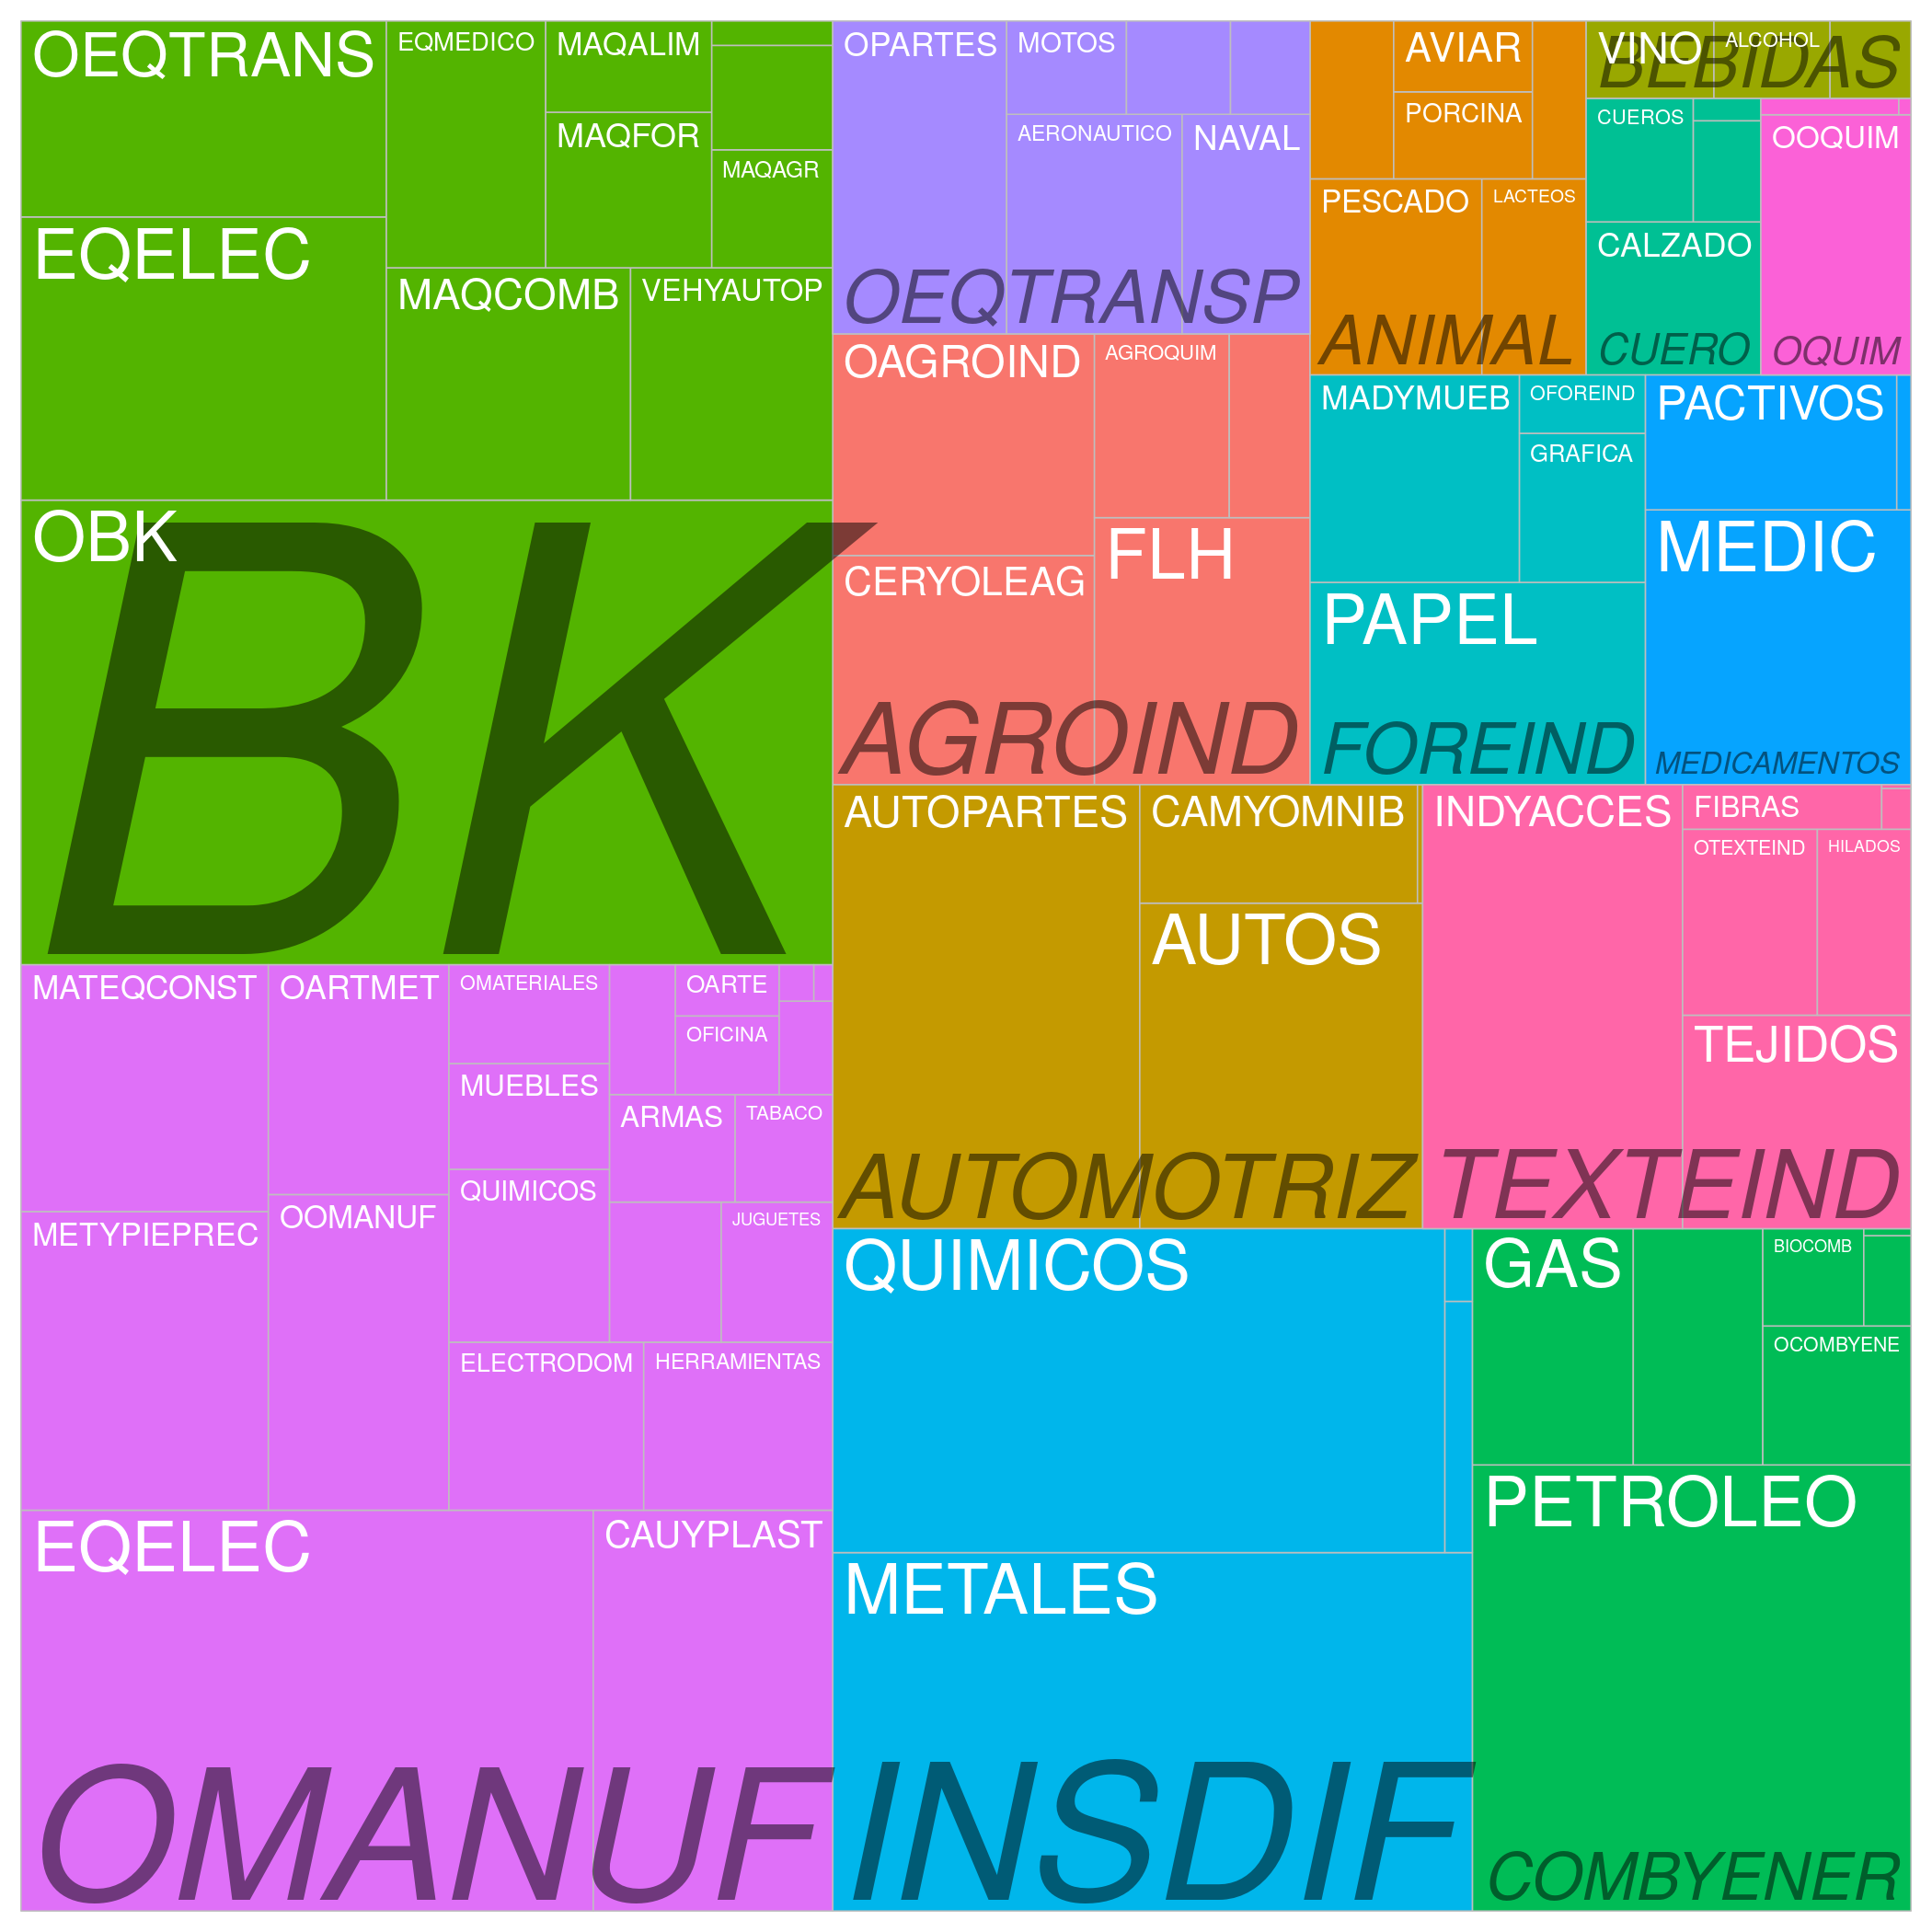
\includegraphics[width=.65\linewidth]{treemap_cadsubcad.png}}
		\subfigure[Cadenas y Usos]{\label{fig:treemaps_global_2}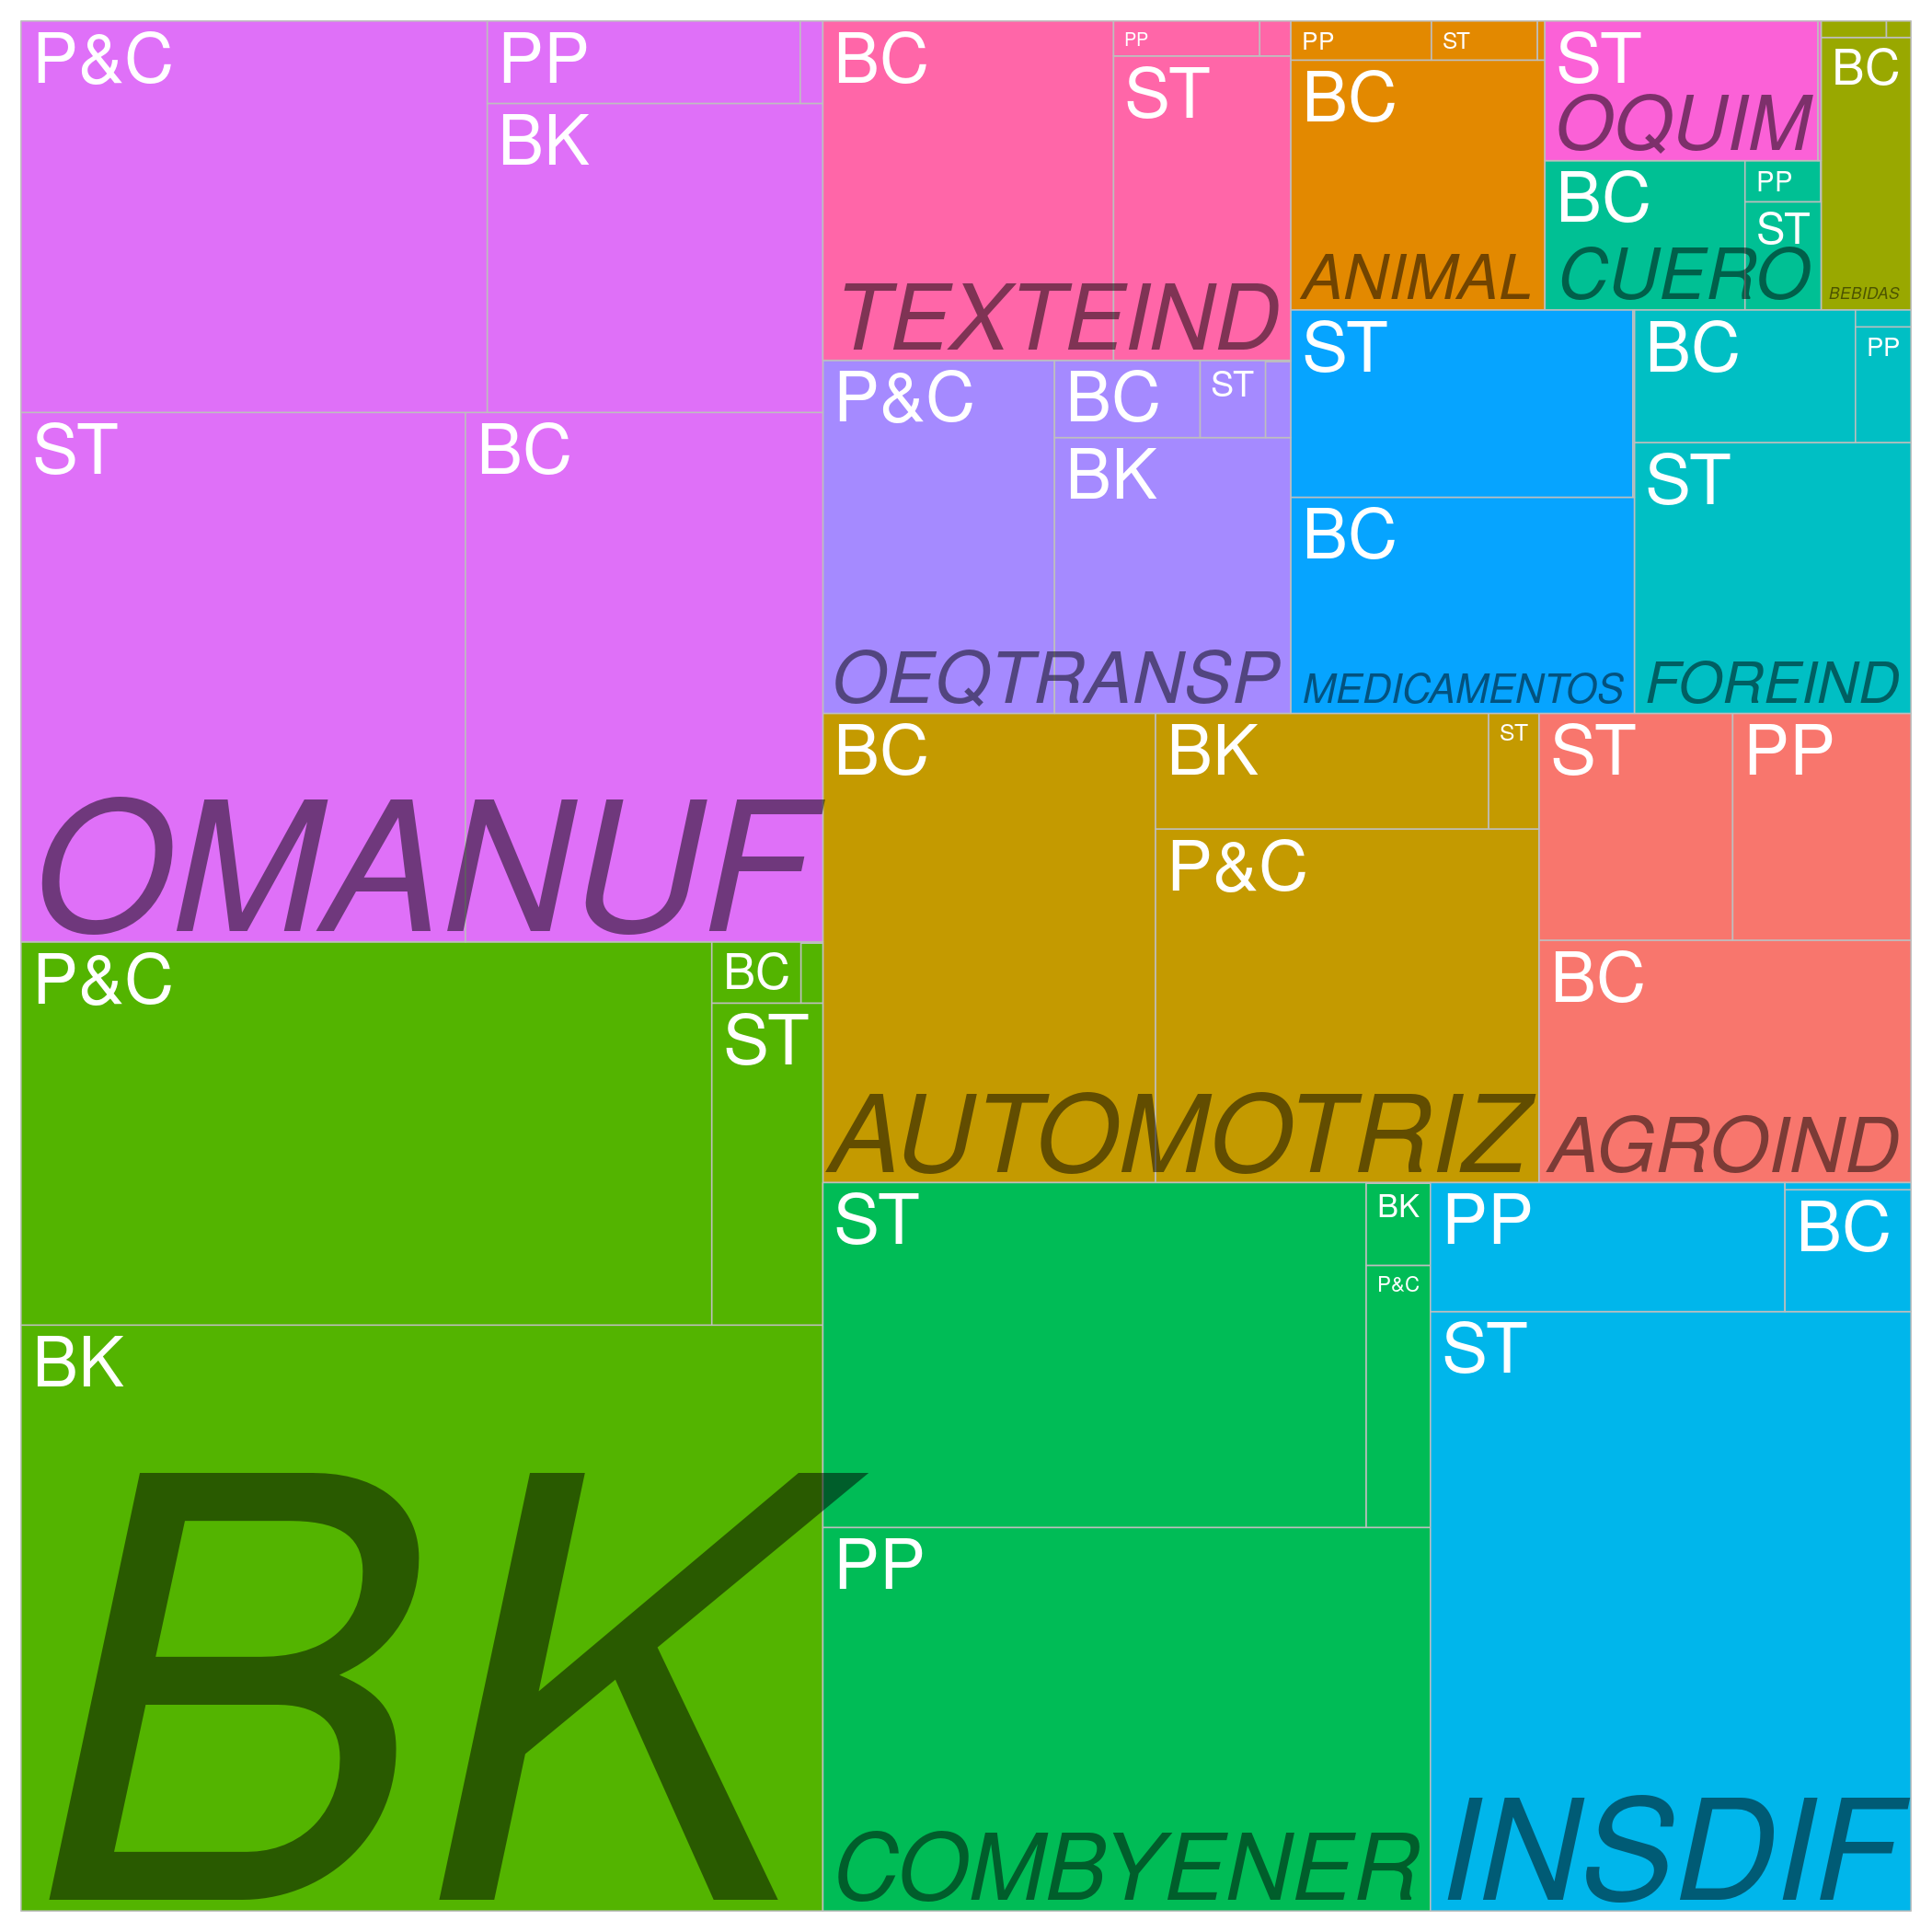
\includegraphics[width=.65\linewidth]{treemap_usos.png}}
		\caption{Treemaps por tipos de productos. Exportaciones. 1996-2016. Total mundial}
		\label{fig:treemaps_global}
	\end{figure}
	
	
	
	La figura \ref{fig:treemaps_global_paises} muestra la distribución de las exportaciones e importaciones según continente y país exportador, para el promedio 1996-2016. Allí destaca el mayor volumen de exportaciones que importaciones de Asia, y el mayor volumen de importaciones que exportaciones de Estados Unidos, siguiendo las mismas conclusiones que el capítulo 2. 
	
	
	\begin{figure}
		\centering
		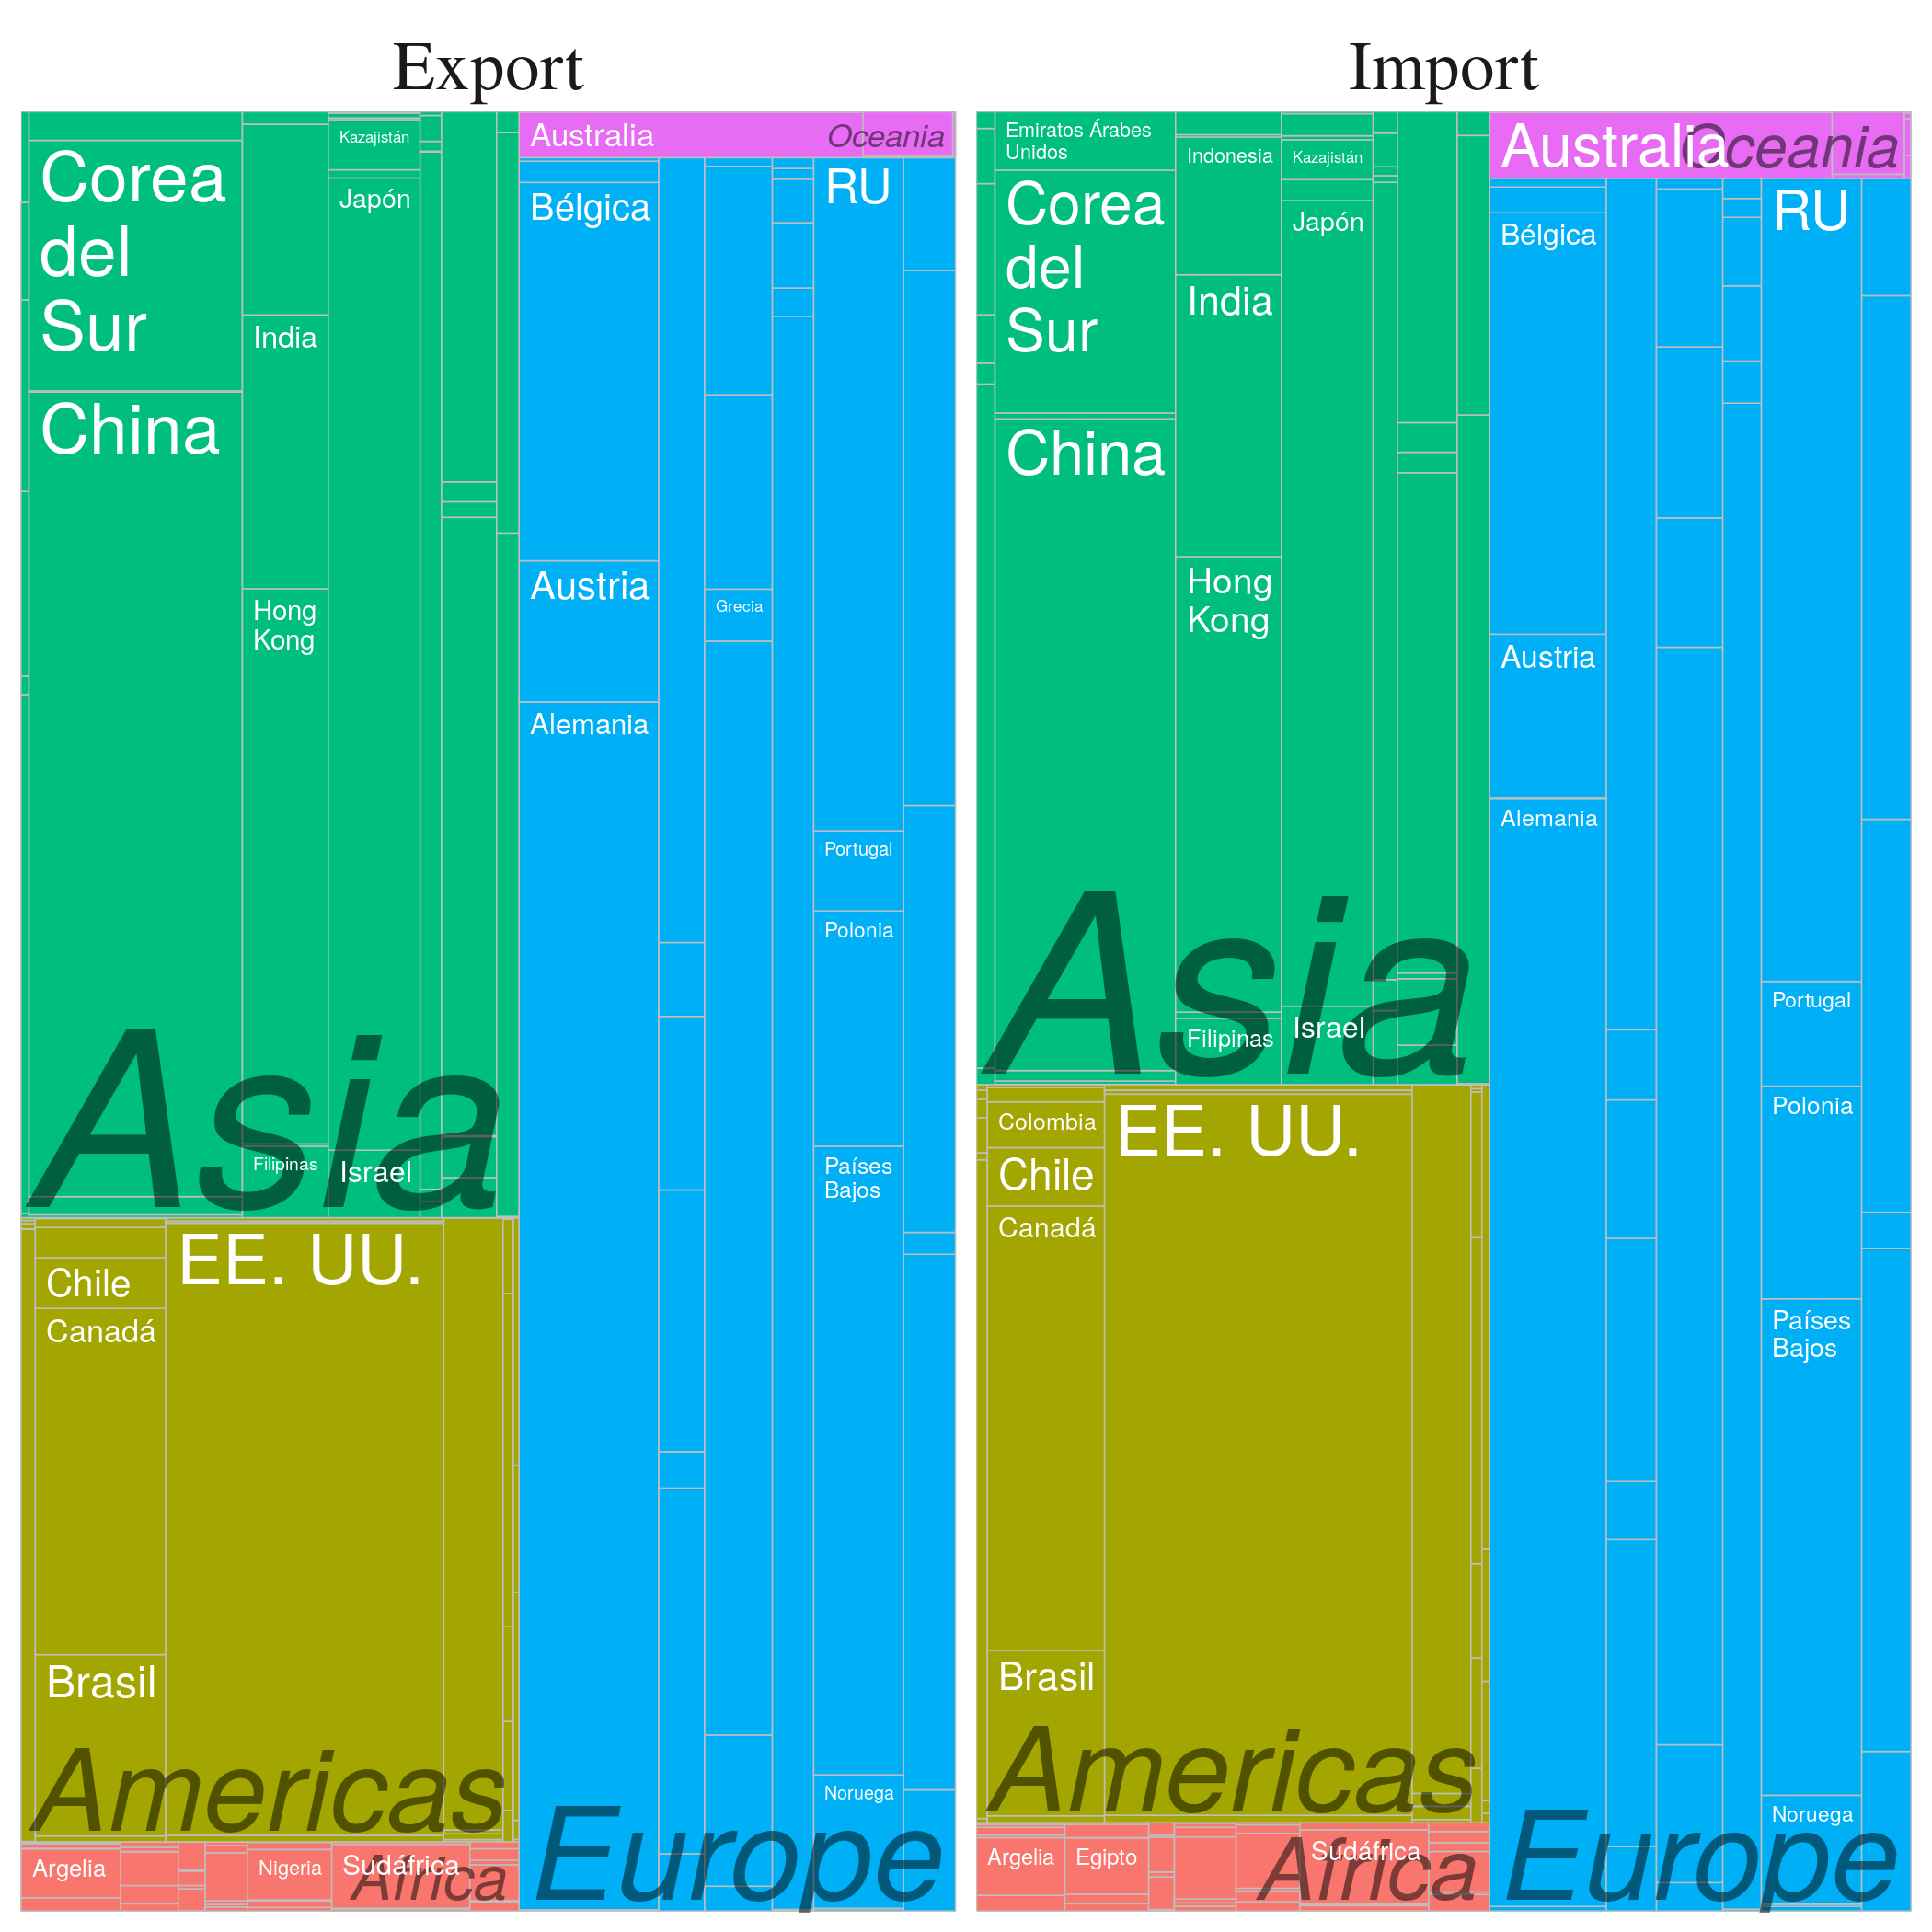
\includegraphics[width=.75\textwidth]{treemap_paises}
		\caption{Treemaps por Continentes y países. 1996-2016. Total mundial}
				\label{fig:treemaps_global_paises}
	\end{figure}
	
	
	Sin embargo, la riqueza en el análisis a nivel producto se encuentra en comprar la distinta composición de la balanza comercial de los países. Ya sea la diferencia entre la composición de sus exportaciones respecto de sus importaciones, como de estos elementos respecto de otros países o regiones. Dado que dicho análisis implica la comparación de una multiplicidad de treemaps, se decidió elaborar una herramienta interactiva para el análisis. La misma fue elaborada utilizando la librería \textit{shiny} \citep{Chang2018} y se encuentra disponible en \hyperlink{https://treemaps.shinyapps.io/treemaps/}{https://treemaps.shinyapps.io/treemaps/}. Dados los límites del servidor y el interés de estudiar la herramienta para un caso específico, el análisis se centra en el caso latinoamericano, tanto para el subcontinente en conjunto como para los países que lo integran. El objeto de análisis es estudiar las posibilidades de integración regional de la producción, y para ello analizar el comportamiento diferencial de las canastas exportadoras e importadoras de los países latinoamericanos cuando comercian entre sí respecto de su comercio con el resto del mundo. A su vez, dada la importancia del comercio de esta región con China, se decidió dividir la información del resto del mundo exceptuando a China y este país de forma individual.
	
	En la figura \ref{fig:treemaps_sudamerica_cadsubcad} se pueden observar los treemaps de cadenas y subcadenas para 2016 del total de los países sudamericanos, según su destino. En la figura \ref{fig:treemaps_sudamerica_cadsubcad_1} se ve como la canasta exportadora de los países latinoamericanos varía según si su destino se encuentra dentro o fuera de la región, y en particular si son exportaciones hacia China. En particular, el comercio intra-regional tiene un componente importante de bienes de capital, y del sector automotriz, ya sean autos terminados o autopartes. Por su parte, en el comercio con el resto del mundo estos componentes cumplen un rol secundario, mientras que se destacan las cadenas agroindustriales, de combustibles e insumos industriales. Respecto del resto del mundo, el comercio con China resalta por las exportaciones de la subcadena de biocombusitbles, cereales y oleaginosas y Metales. 
	Las importaciones de estos mismos países se pueden observar en la figura \ref{fig:treemaps_sudamerica_cadsubcad_2}. Naturalmente los treemaps de las exportaciones e importaciones son muy similares, ya que la única diferencia es el país que registra la operación. Sin embargo, en las importaciones del resto del mundo destacan las cadenas automotriz y de bienes de capital. A su vez, resulta de interés el cambio de composición de las cadenas: Mientras que las exportaciones de insumos industriales hacia el resto del mundo son mayoritariamente metales, en las importaciones destacan los productos químicos. Por su parte, mientras que en la cadena de otras manufacturas se exportan hacia el resto del mundo metales y piedras preciosas, se importan dentro de esta cadena equipos eléctricos. A su vez, del resto del mundo se importan medicamentos, aunque este rubro no aparece en el treemap de las exportaciones. Cabe destacar que la región exporta e importa petróleo hacia el resto del mundo, aunque el comercio intrarregional de este producto es menor. Existe, por lo tanto, una potencialidad de integración comercial dentro de la región para este producto en particular. 
	El comercio con China esta particularmente orientado a la venta de materias primas y la compra de productos industriales. Destacan especialmente las exportaciones de cereales y oleaginosas, biocombustibles y metales; mientras que se importan equipos eléctricos, bienes de capital, calzados y químicos. 
	

\begin{figure}
	\centering
	\subfigure[Exportaciones]{\label{fig:treemaps_sudamerica_cadsubcad_1}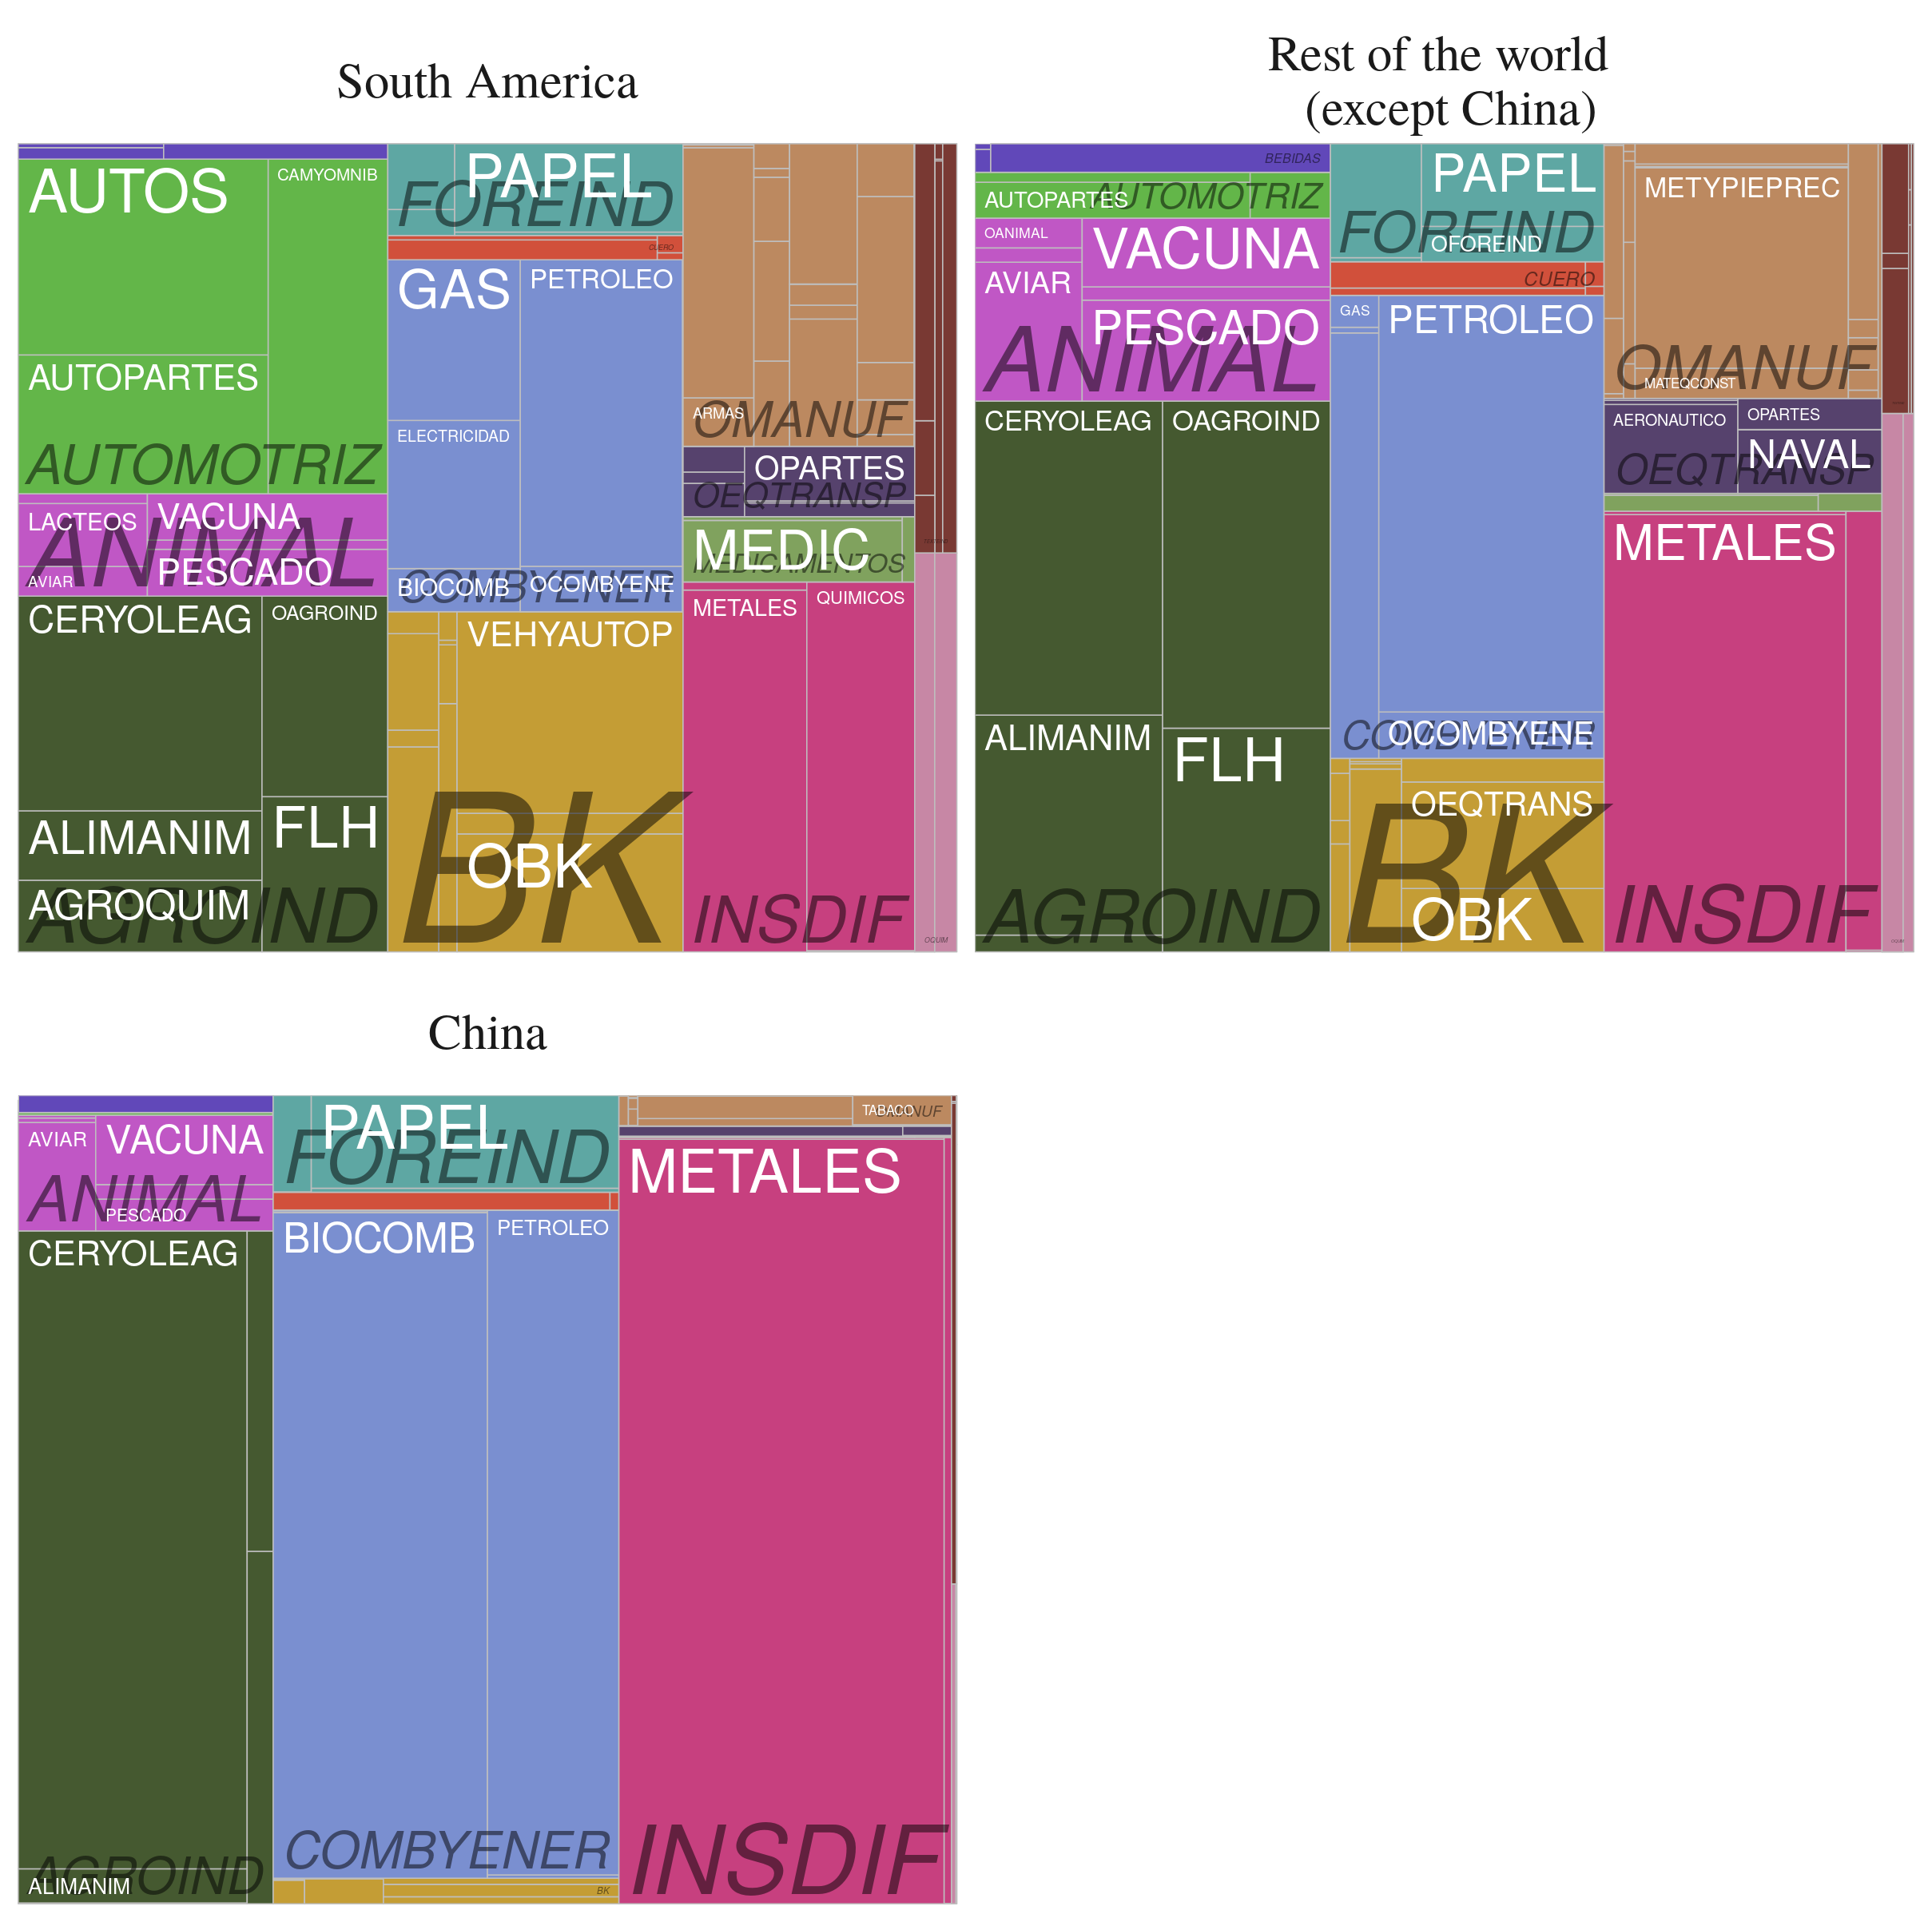
\includegraphics[width=.75\linewidth]{treemaps_cadsubcad2016}}
	\subfigure[Importaciones]{\label{fig:treemaps_sudamerica_cadsubcad_2}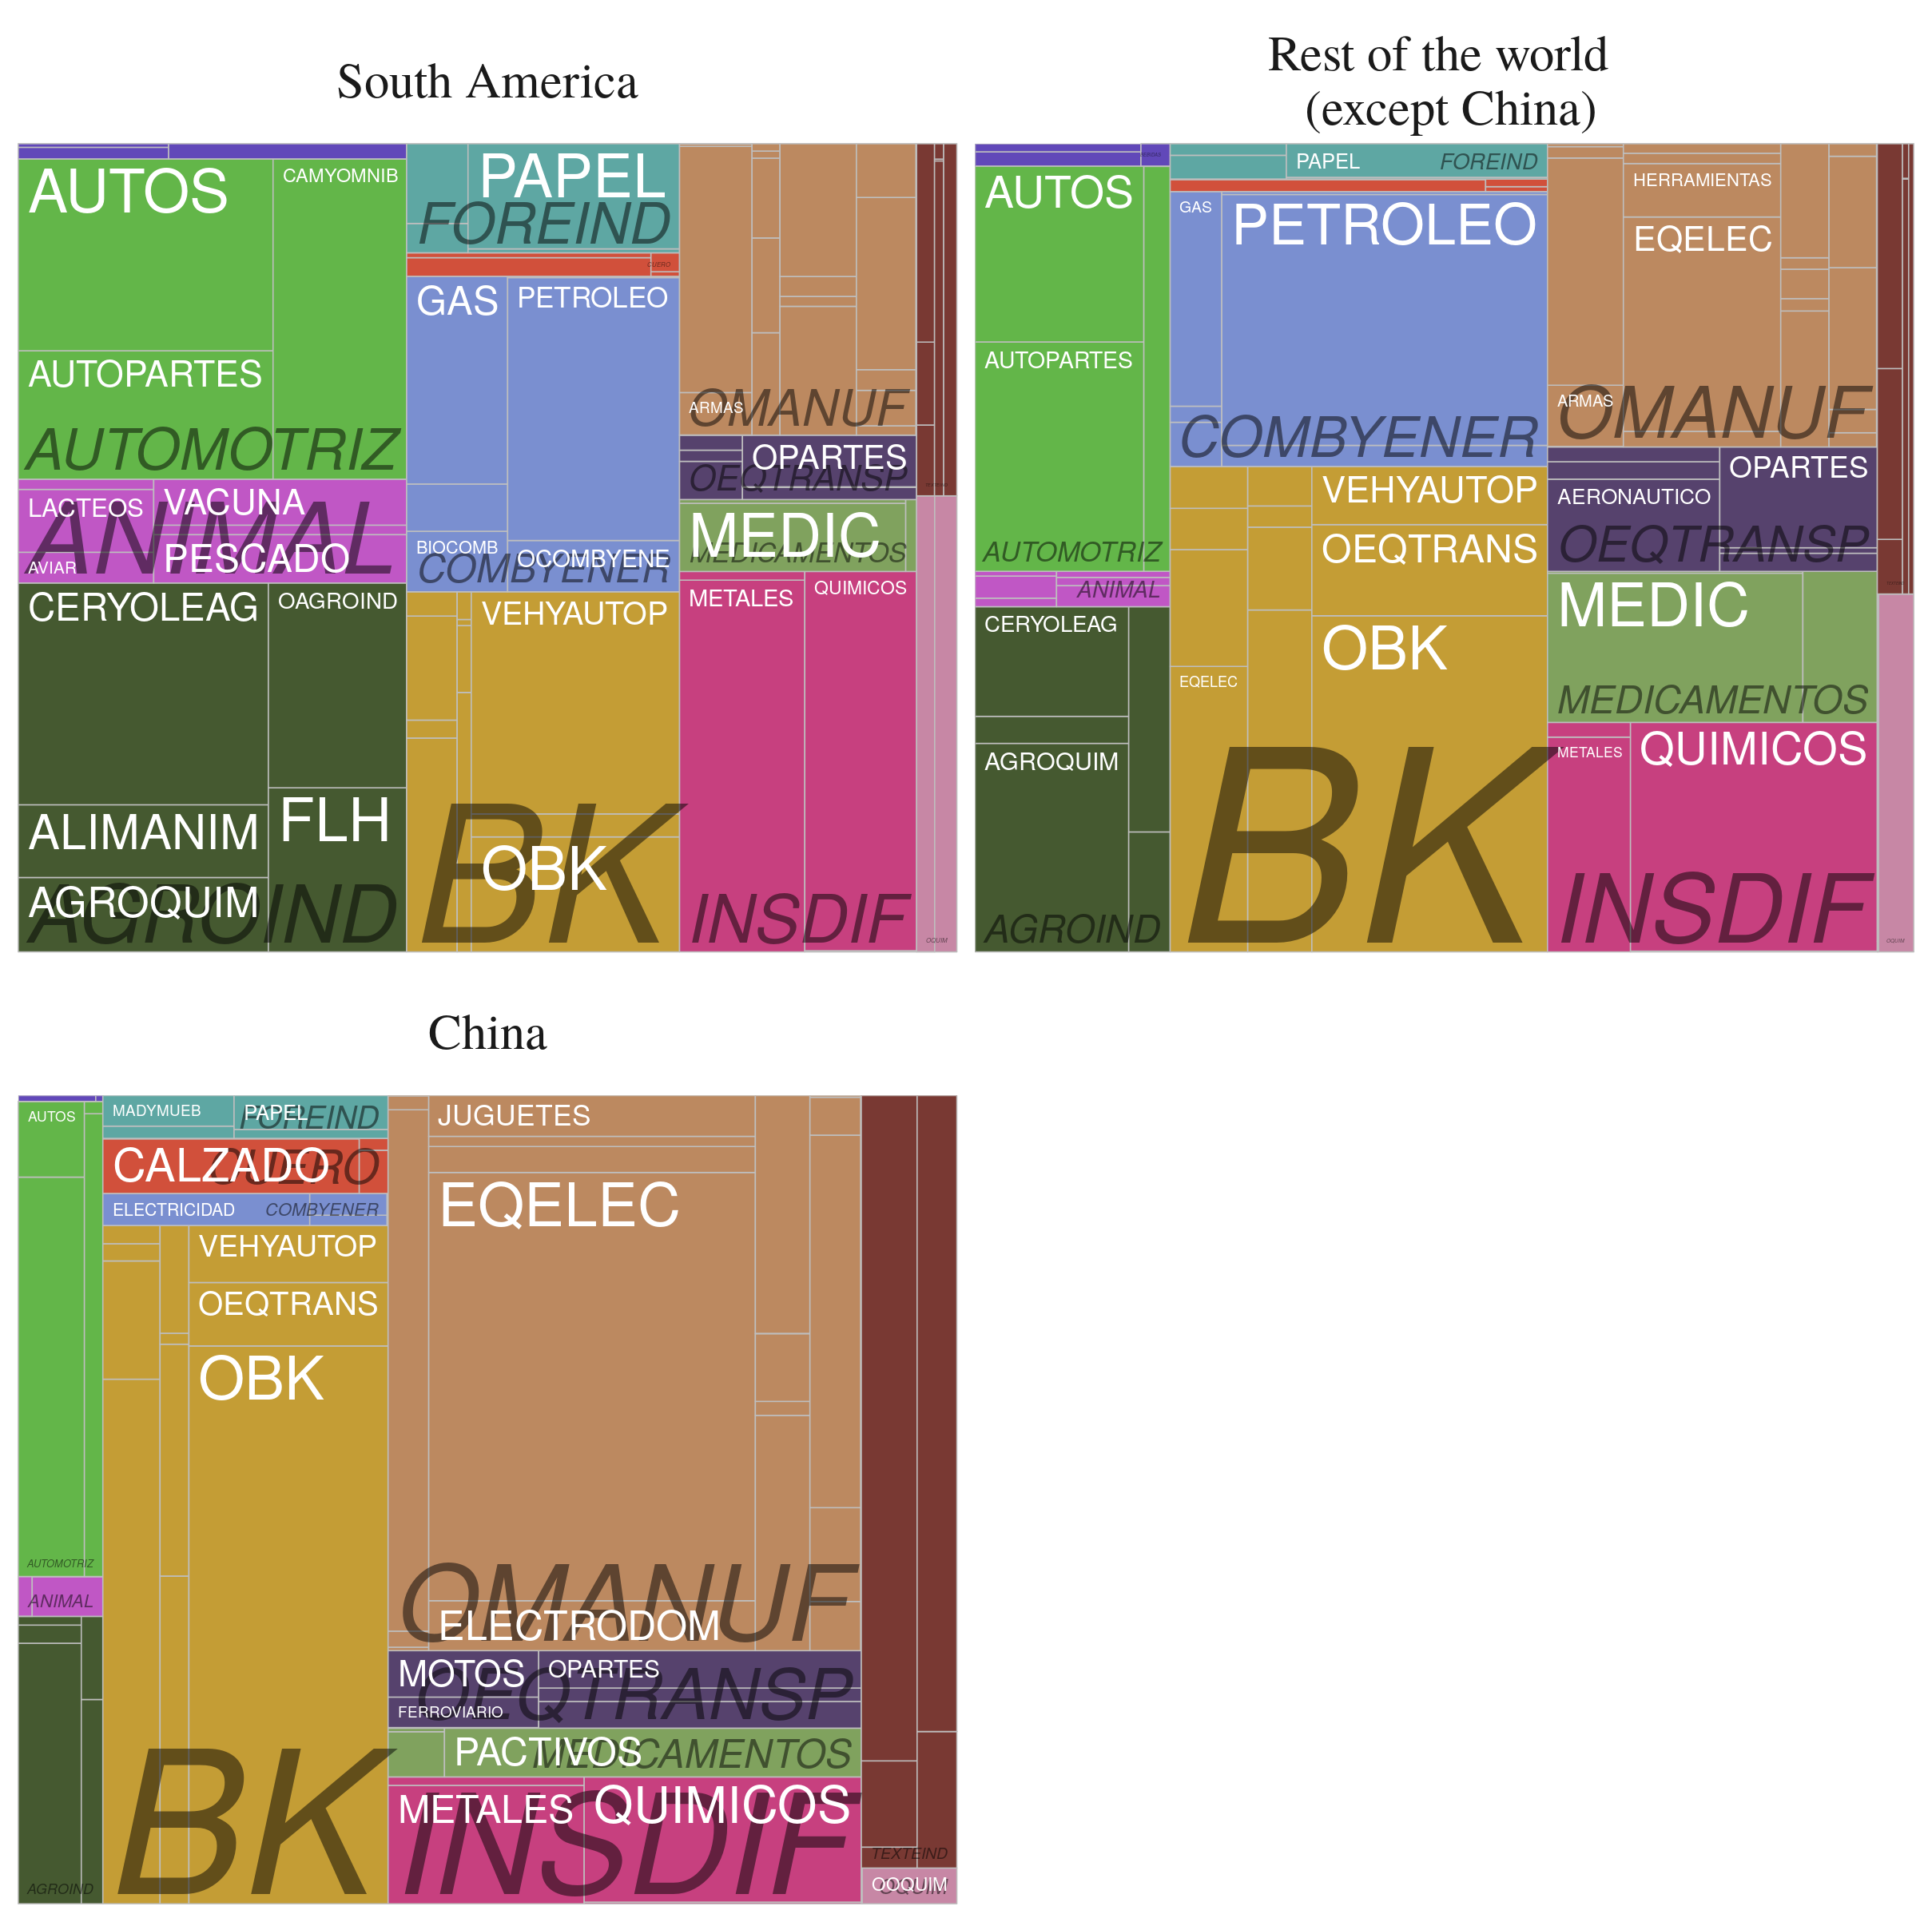
\includegraphics[width=.75\linewidth]{treemaps_cadsubcad2016_impos}}
	\caption{Treemaps de Cadenas y Subcadenas.2016. Total Latinoamérica}
	\label{fig:treemaps_sudamerica_cadsubcad}
\end{figure}


La figura \ref{fig:treemaps_sudamerica_usos} muestra los treemaps exclusivamente según los usos de los productos, para el total de la región, según su destino, en el año 2016. En \ref{fig:treemaps_sudamerica_usos_1} se puede observar las exportaciones. Los usos de los productos exportados varían fuertemente según su destino. Los productos semiterminados constituyen la mayoría de las exportaciones tanto hacia el interior de la región, como con el resto del mundo. Sin embargo, mientras que los bienes de consumo resultan de particular importancia dentro de la región, los productos primarios lo son respecto del resto del mundo. El comercio con china destaca esta tendencia, donde la mayoría de las exportaciones provienen de productos primarios. En \ref{fig:treemaps_sudamerica_usos_2} se observa la distribución de las importaciones según su uso. Allí se ve que las importaciones de productos semiterminados desde el resto del mundo supera a las exportaciones, si se lo compara con \ref{fig:treemaps_sudamerica_usos_1}. A su vez, prácticamente no se exportan productos primarios, pero sí partes y componentes, y bienes de capital. El comercio con China se encuentra equitativamente distribuido entre bienes de capital, productos semiterminados, de consumo y partes y componentes. Es notorio que no se importa prácticamente productos primarios, aunque estos constituyen la base de las exportaciones a dicho país. 

\begin{figure}
	\centering
	\subfigure[Exportaciones]{\label{fig:treemaps_sudamerica_usos_1}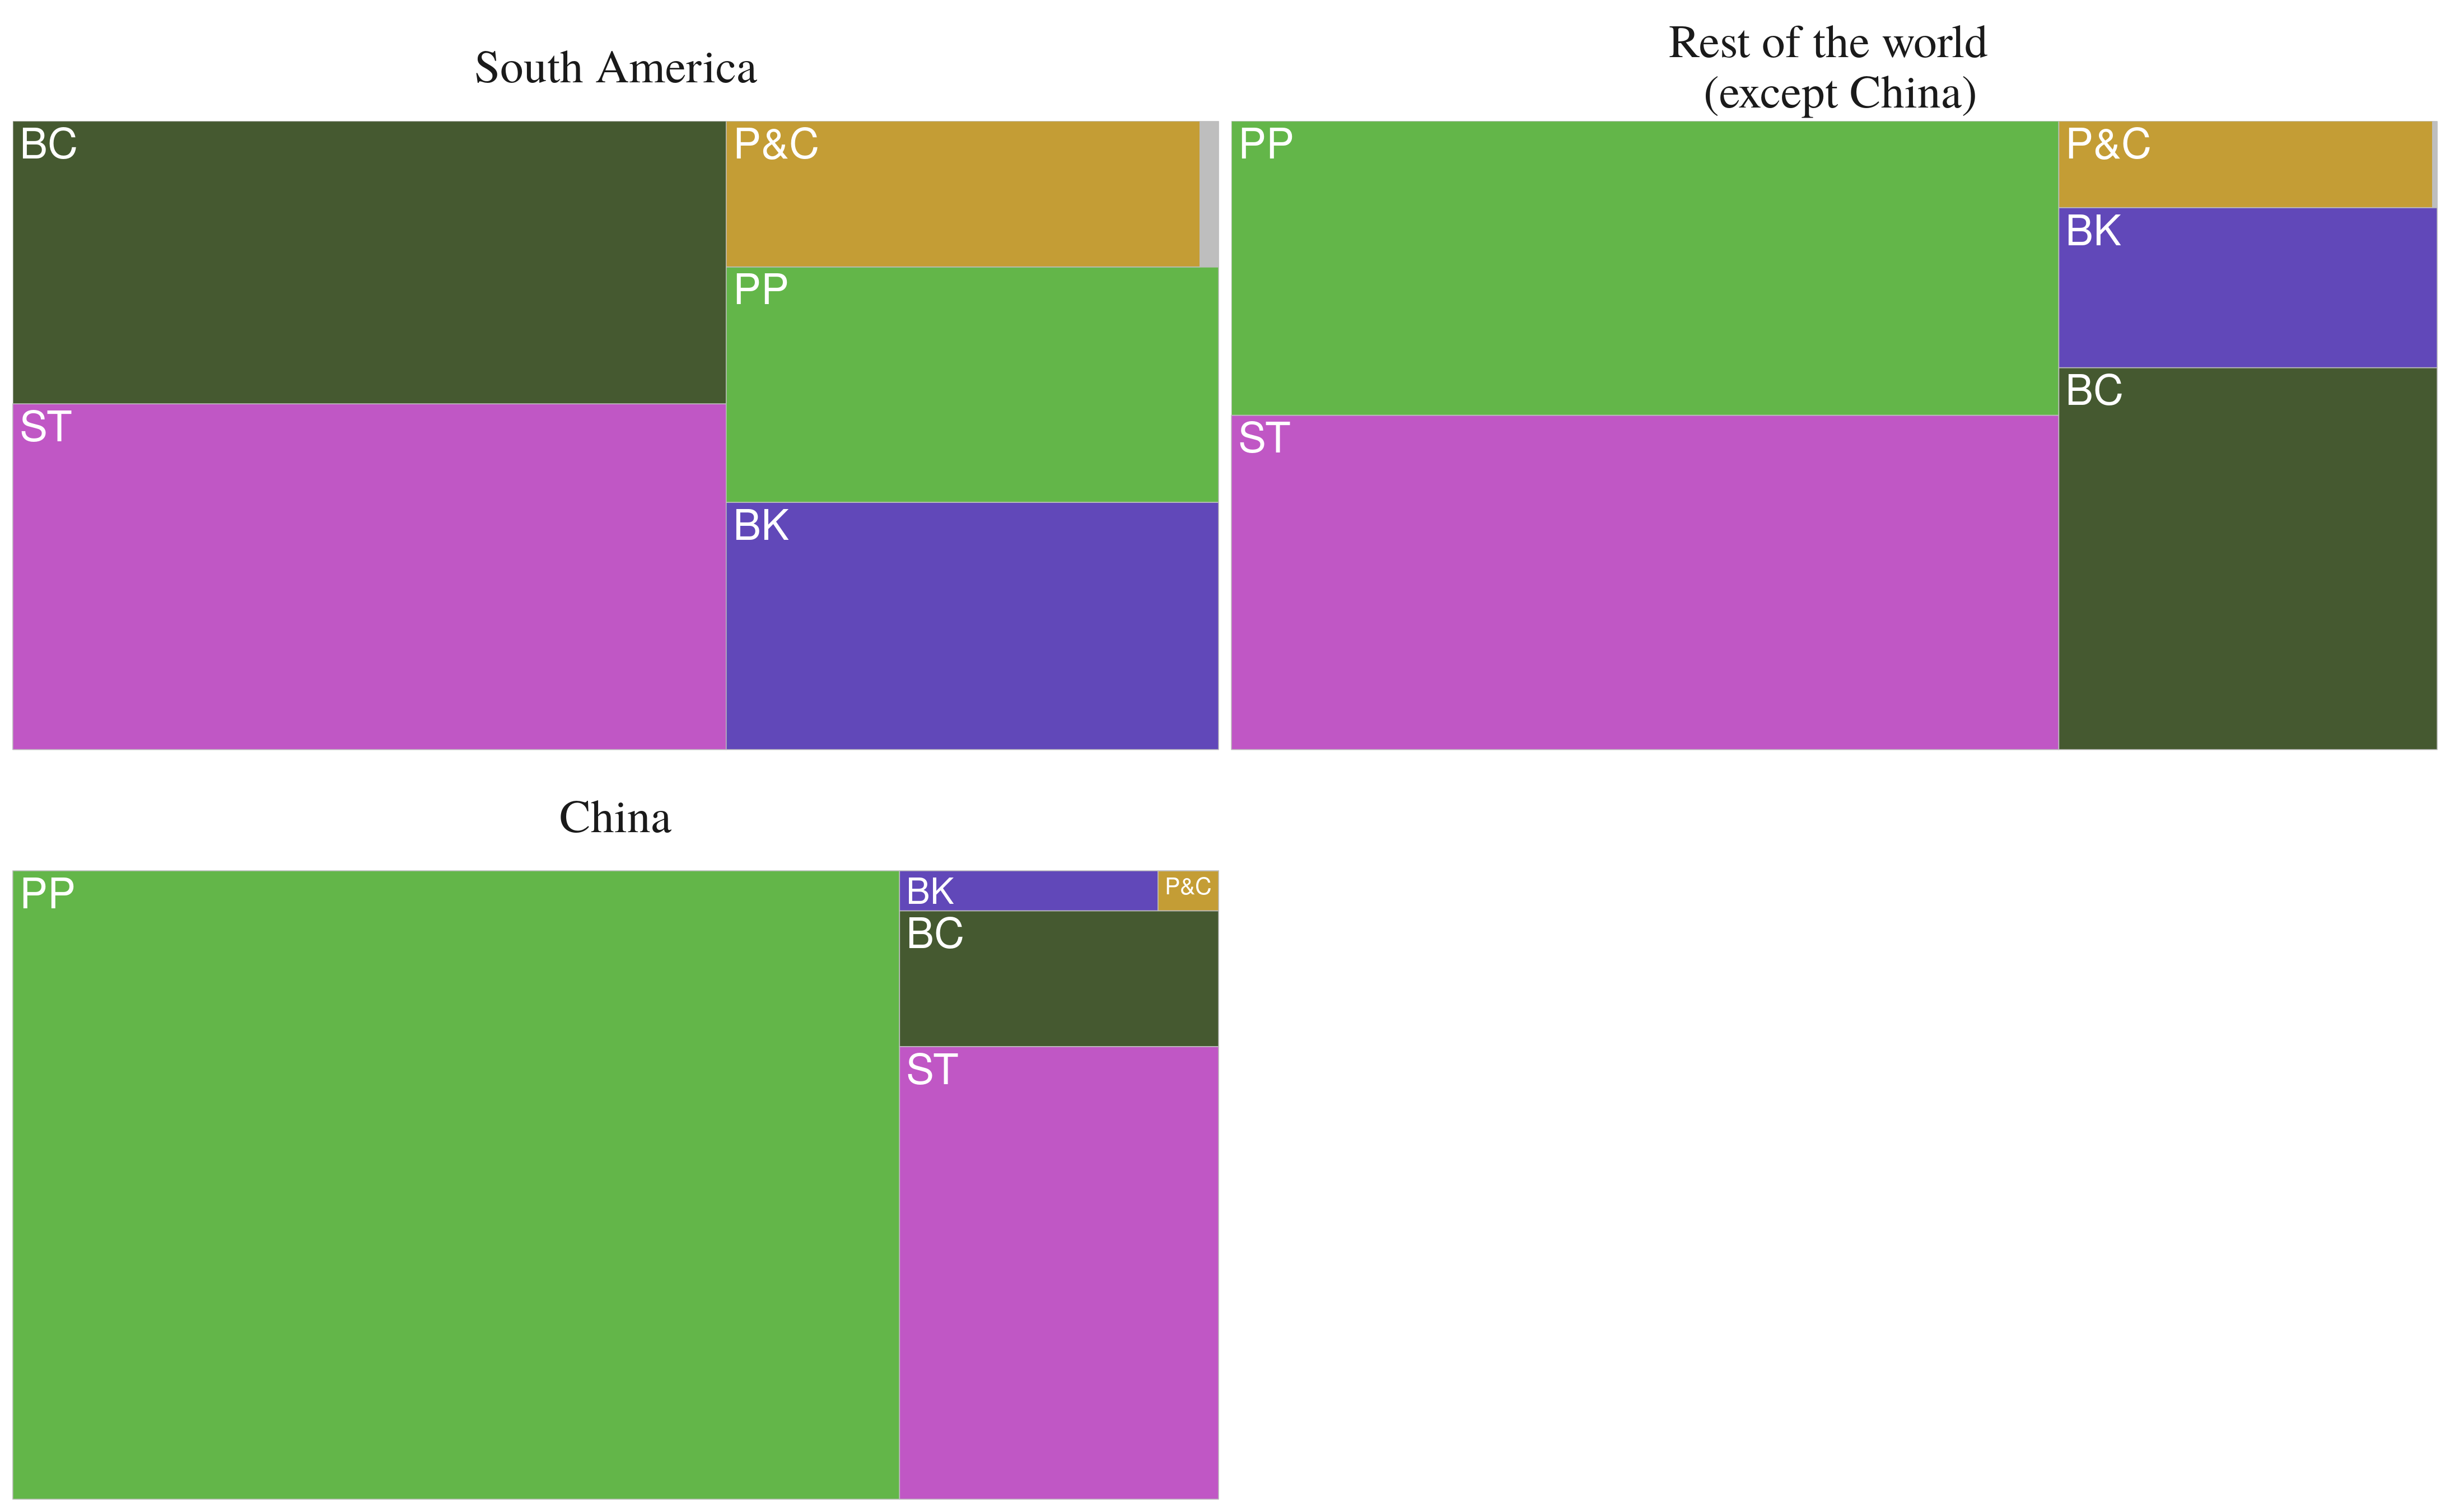
\includegraphics[width=.75\linewidth]{treemaps_usos2016}}
	\subfigure[Importaciones]{\label{fig:treemaps_sudamerica_usos_2}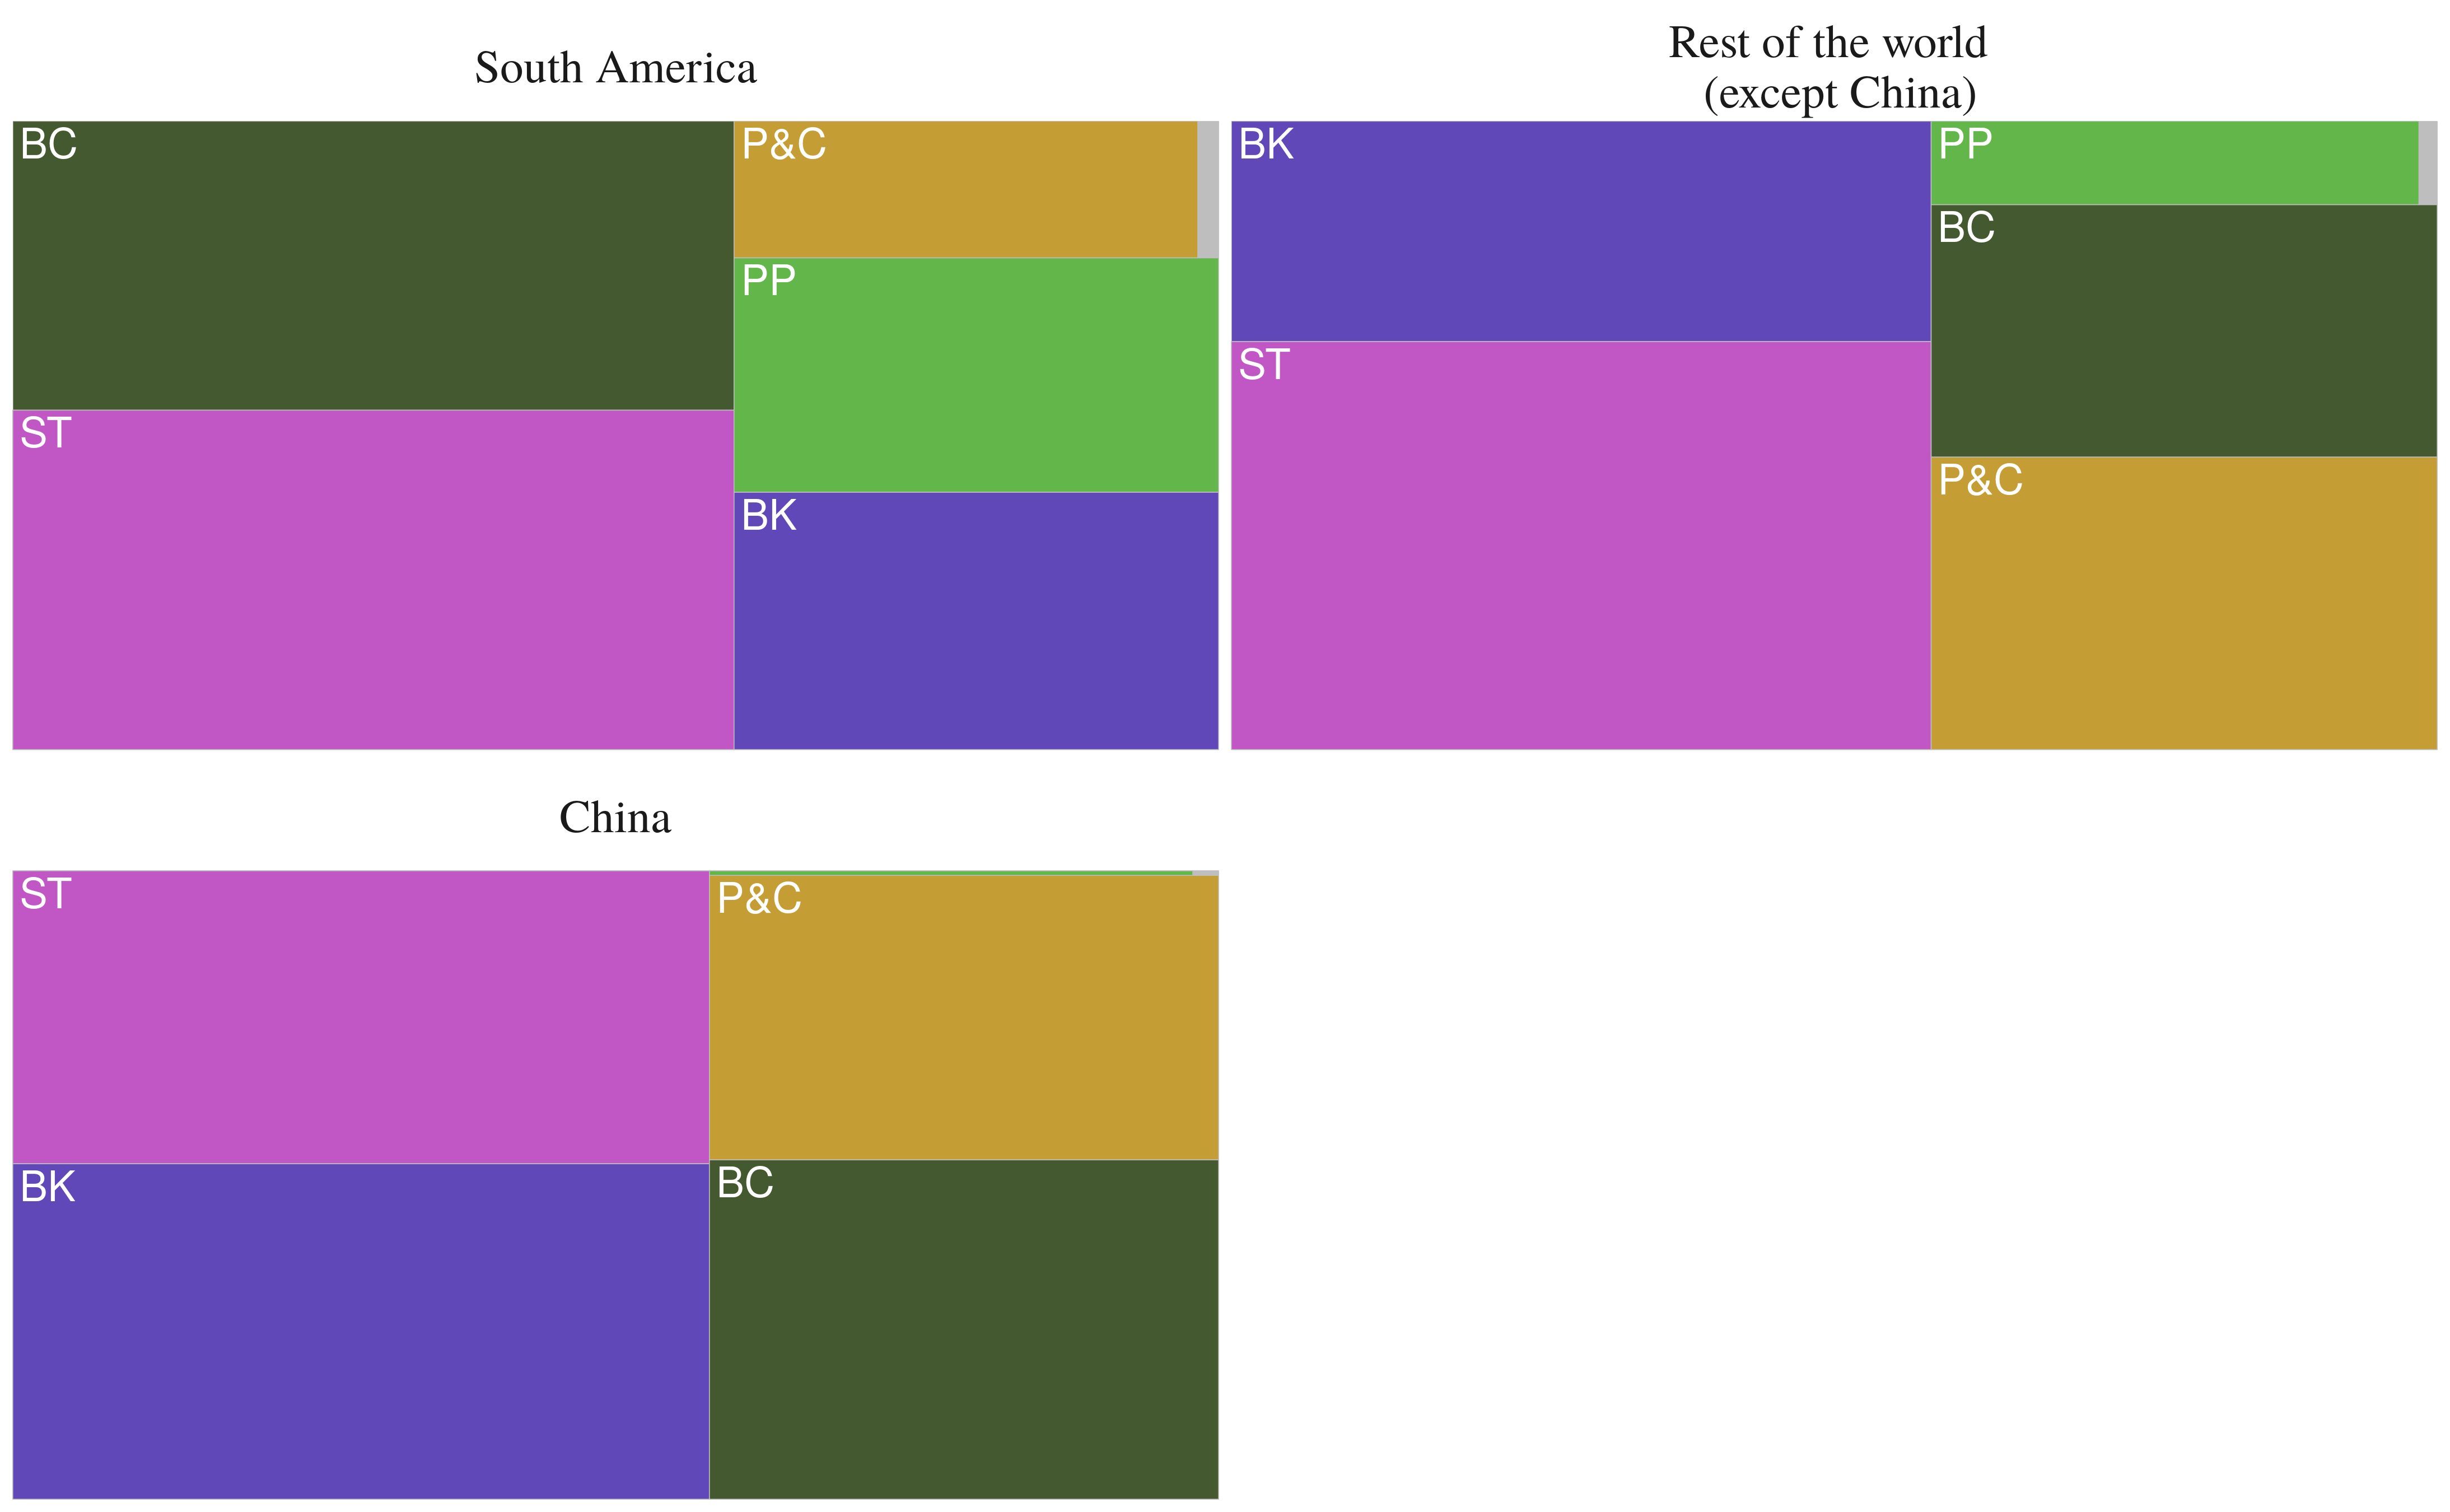
\includegraphics[width=.75\linewidth]{treemaps_usos2016_impos}}
	\caption{Treemaps de Cadenas y Usos.2016. Total Latinoamérica}
	\label{fig:treemaps_sudamerica_usos}
\end{figure}




En la figura \ref{fig:treemaps_sudamerica_destino} se observa la distribución de los socios comerciales de Sudamérica en el 2016. Esto es, los países destino de las exportaciones y origen de las importaciones. En \ref{fig:treemaps_sudamerica_destino_1} se excluye al resto del mundo y China, para observar la distribución interna del comercio. Naturalmente Brasil es el mayor socio comercial interno, para ambos tipos de flujo comercial, aunque su importancia es mucho mayor como exportador que como importador, dado que es el origen del 40\% de las importaciones de los demás países, y el destino del 25\% de las exportaciones. 
En la figura \ref{fig:treemaps_sudamerica_destino_2} se puede observar el mismo gráfico, pero incluyendo al resto del mundo. Allí se ve que tanto las exportaciones como importaciones hacia el resto del mundo exceptuando a China constituyen más de un 60\% del comercio, y China exclusivamente representa casi un 20\% del comercio de la región, superando ampliamente a Brasil. 

\begin{figure}
	\centering
	\subfigure[Excluyendo Resto del Mundo]{\label{fig:treemaps_sudamerica_destino_1}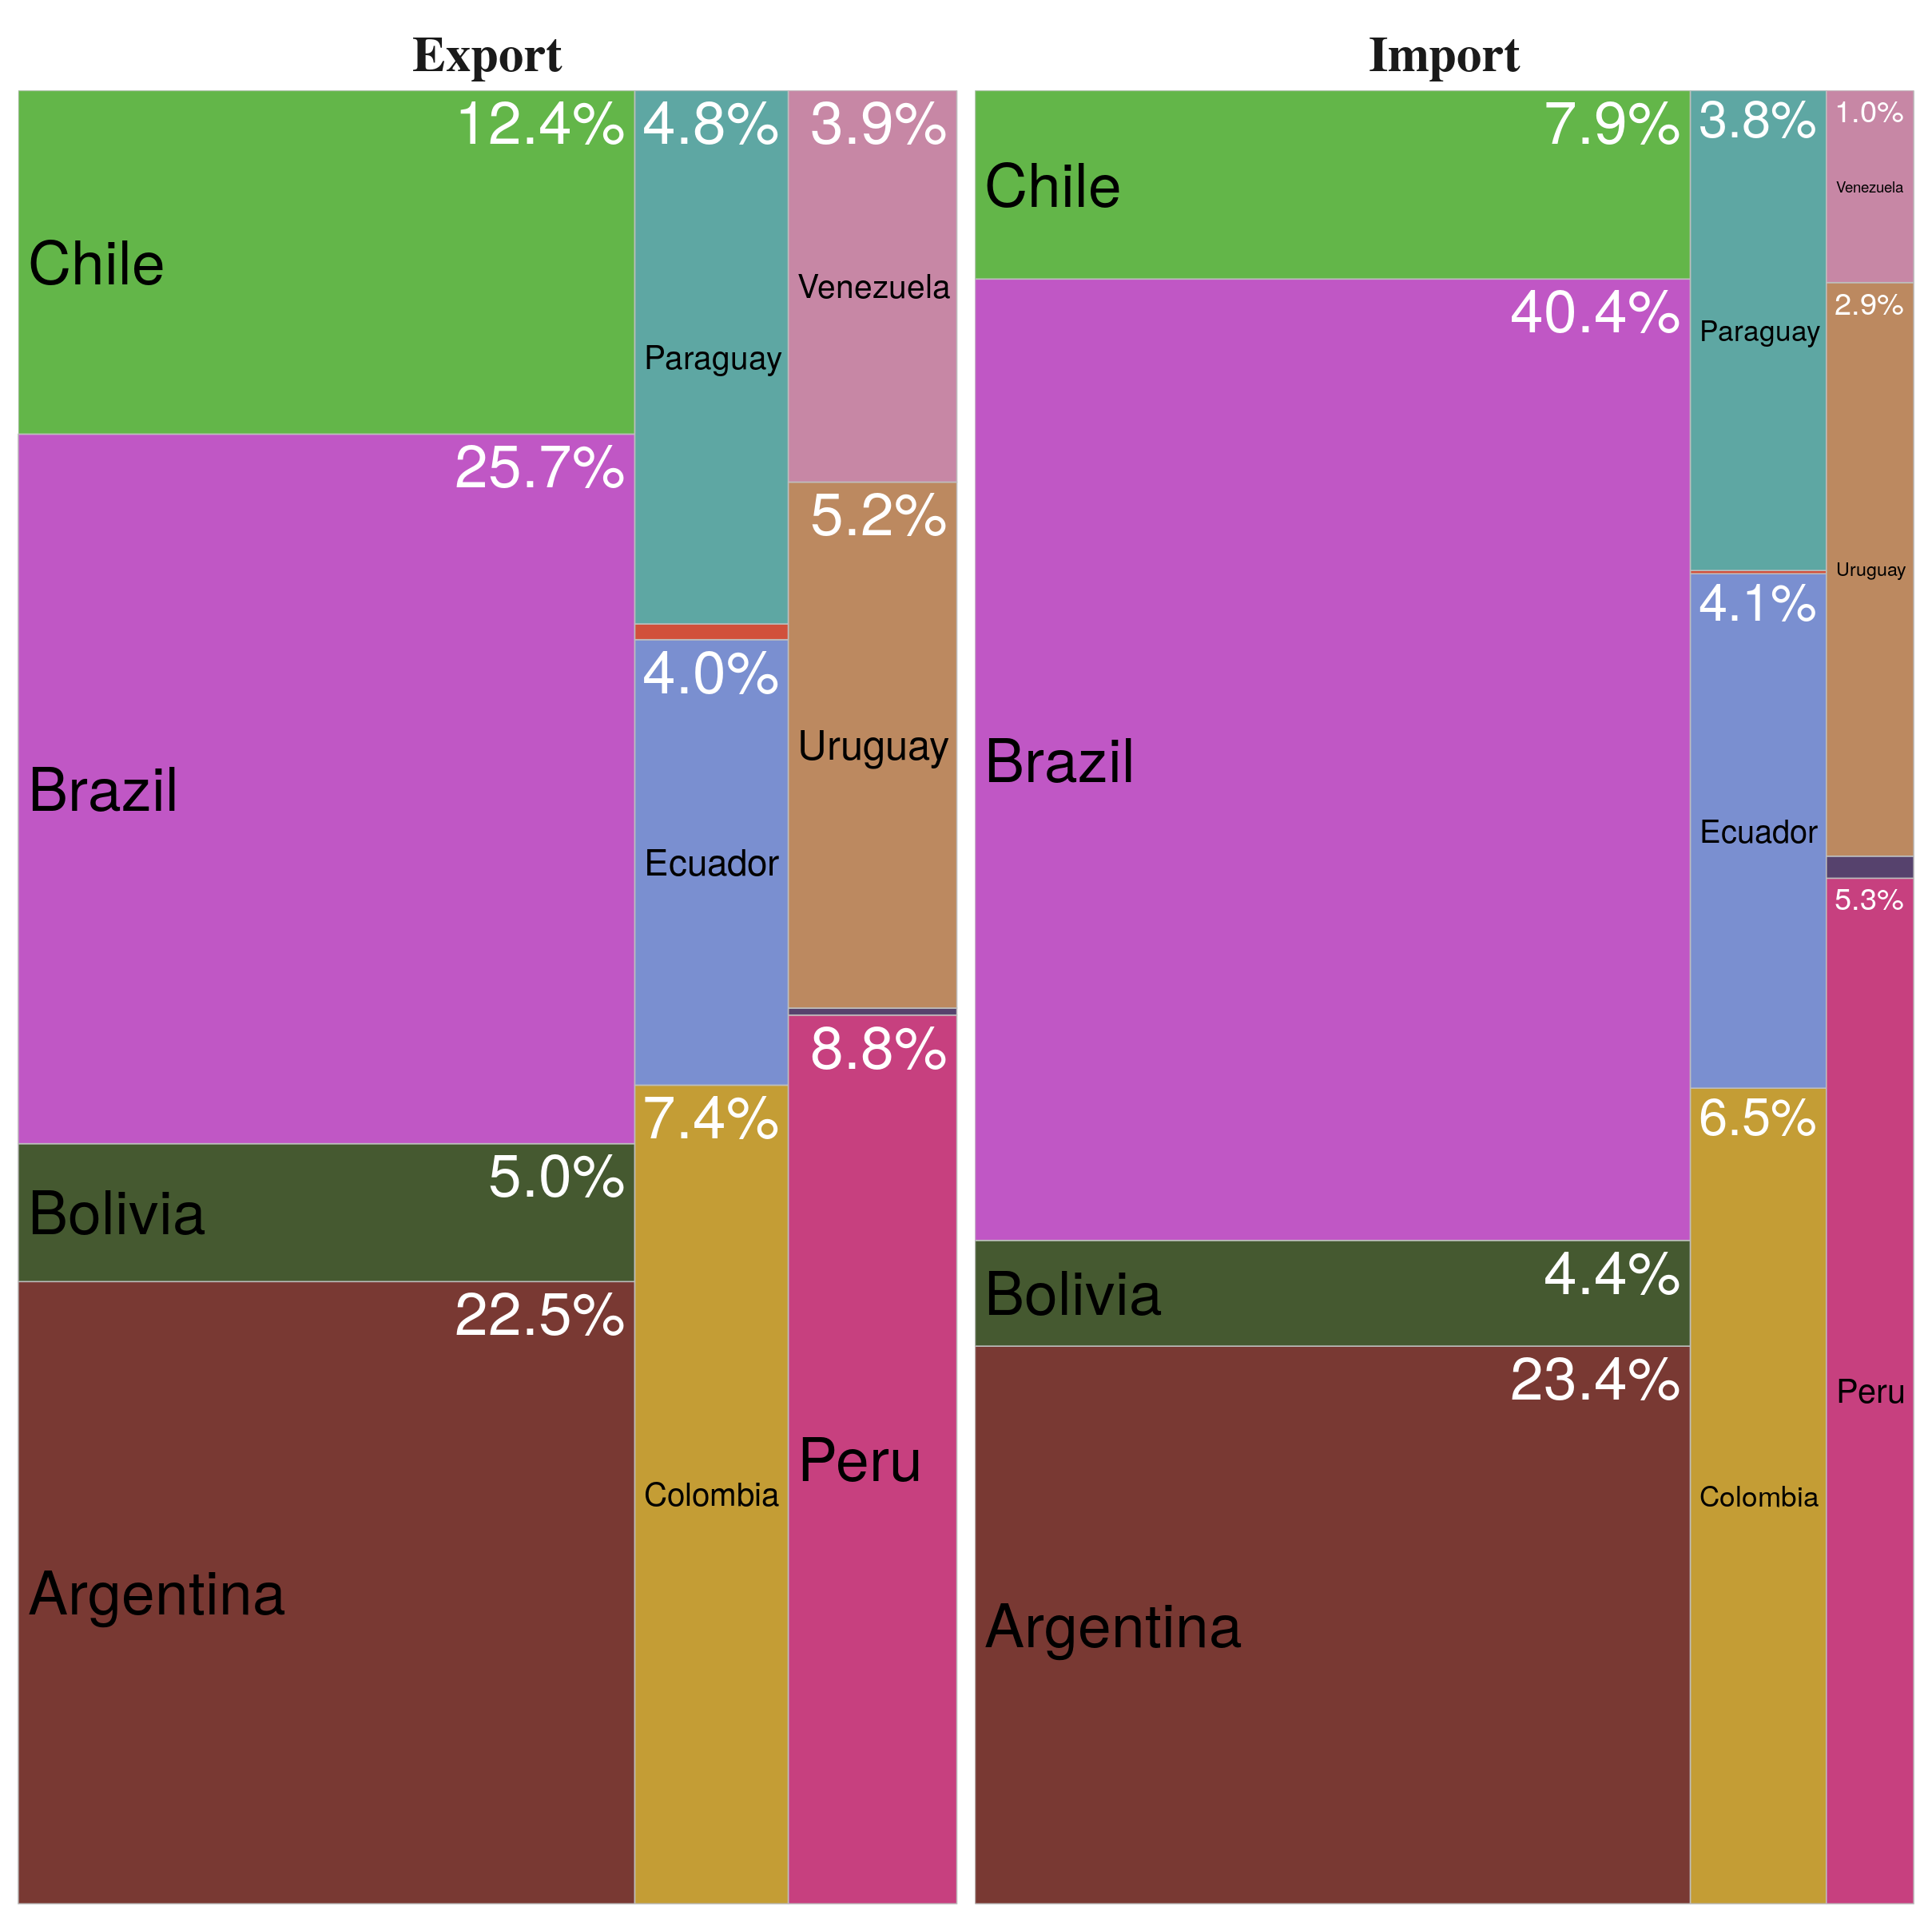
\includegraphics[width=.65\linewidth]{treemaps_paises2016}}
	\subfigure[Incluyendo Resto del mundo]{\label{fig:treemaps_sudamerica_destino_2}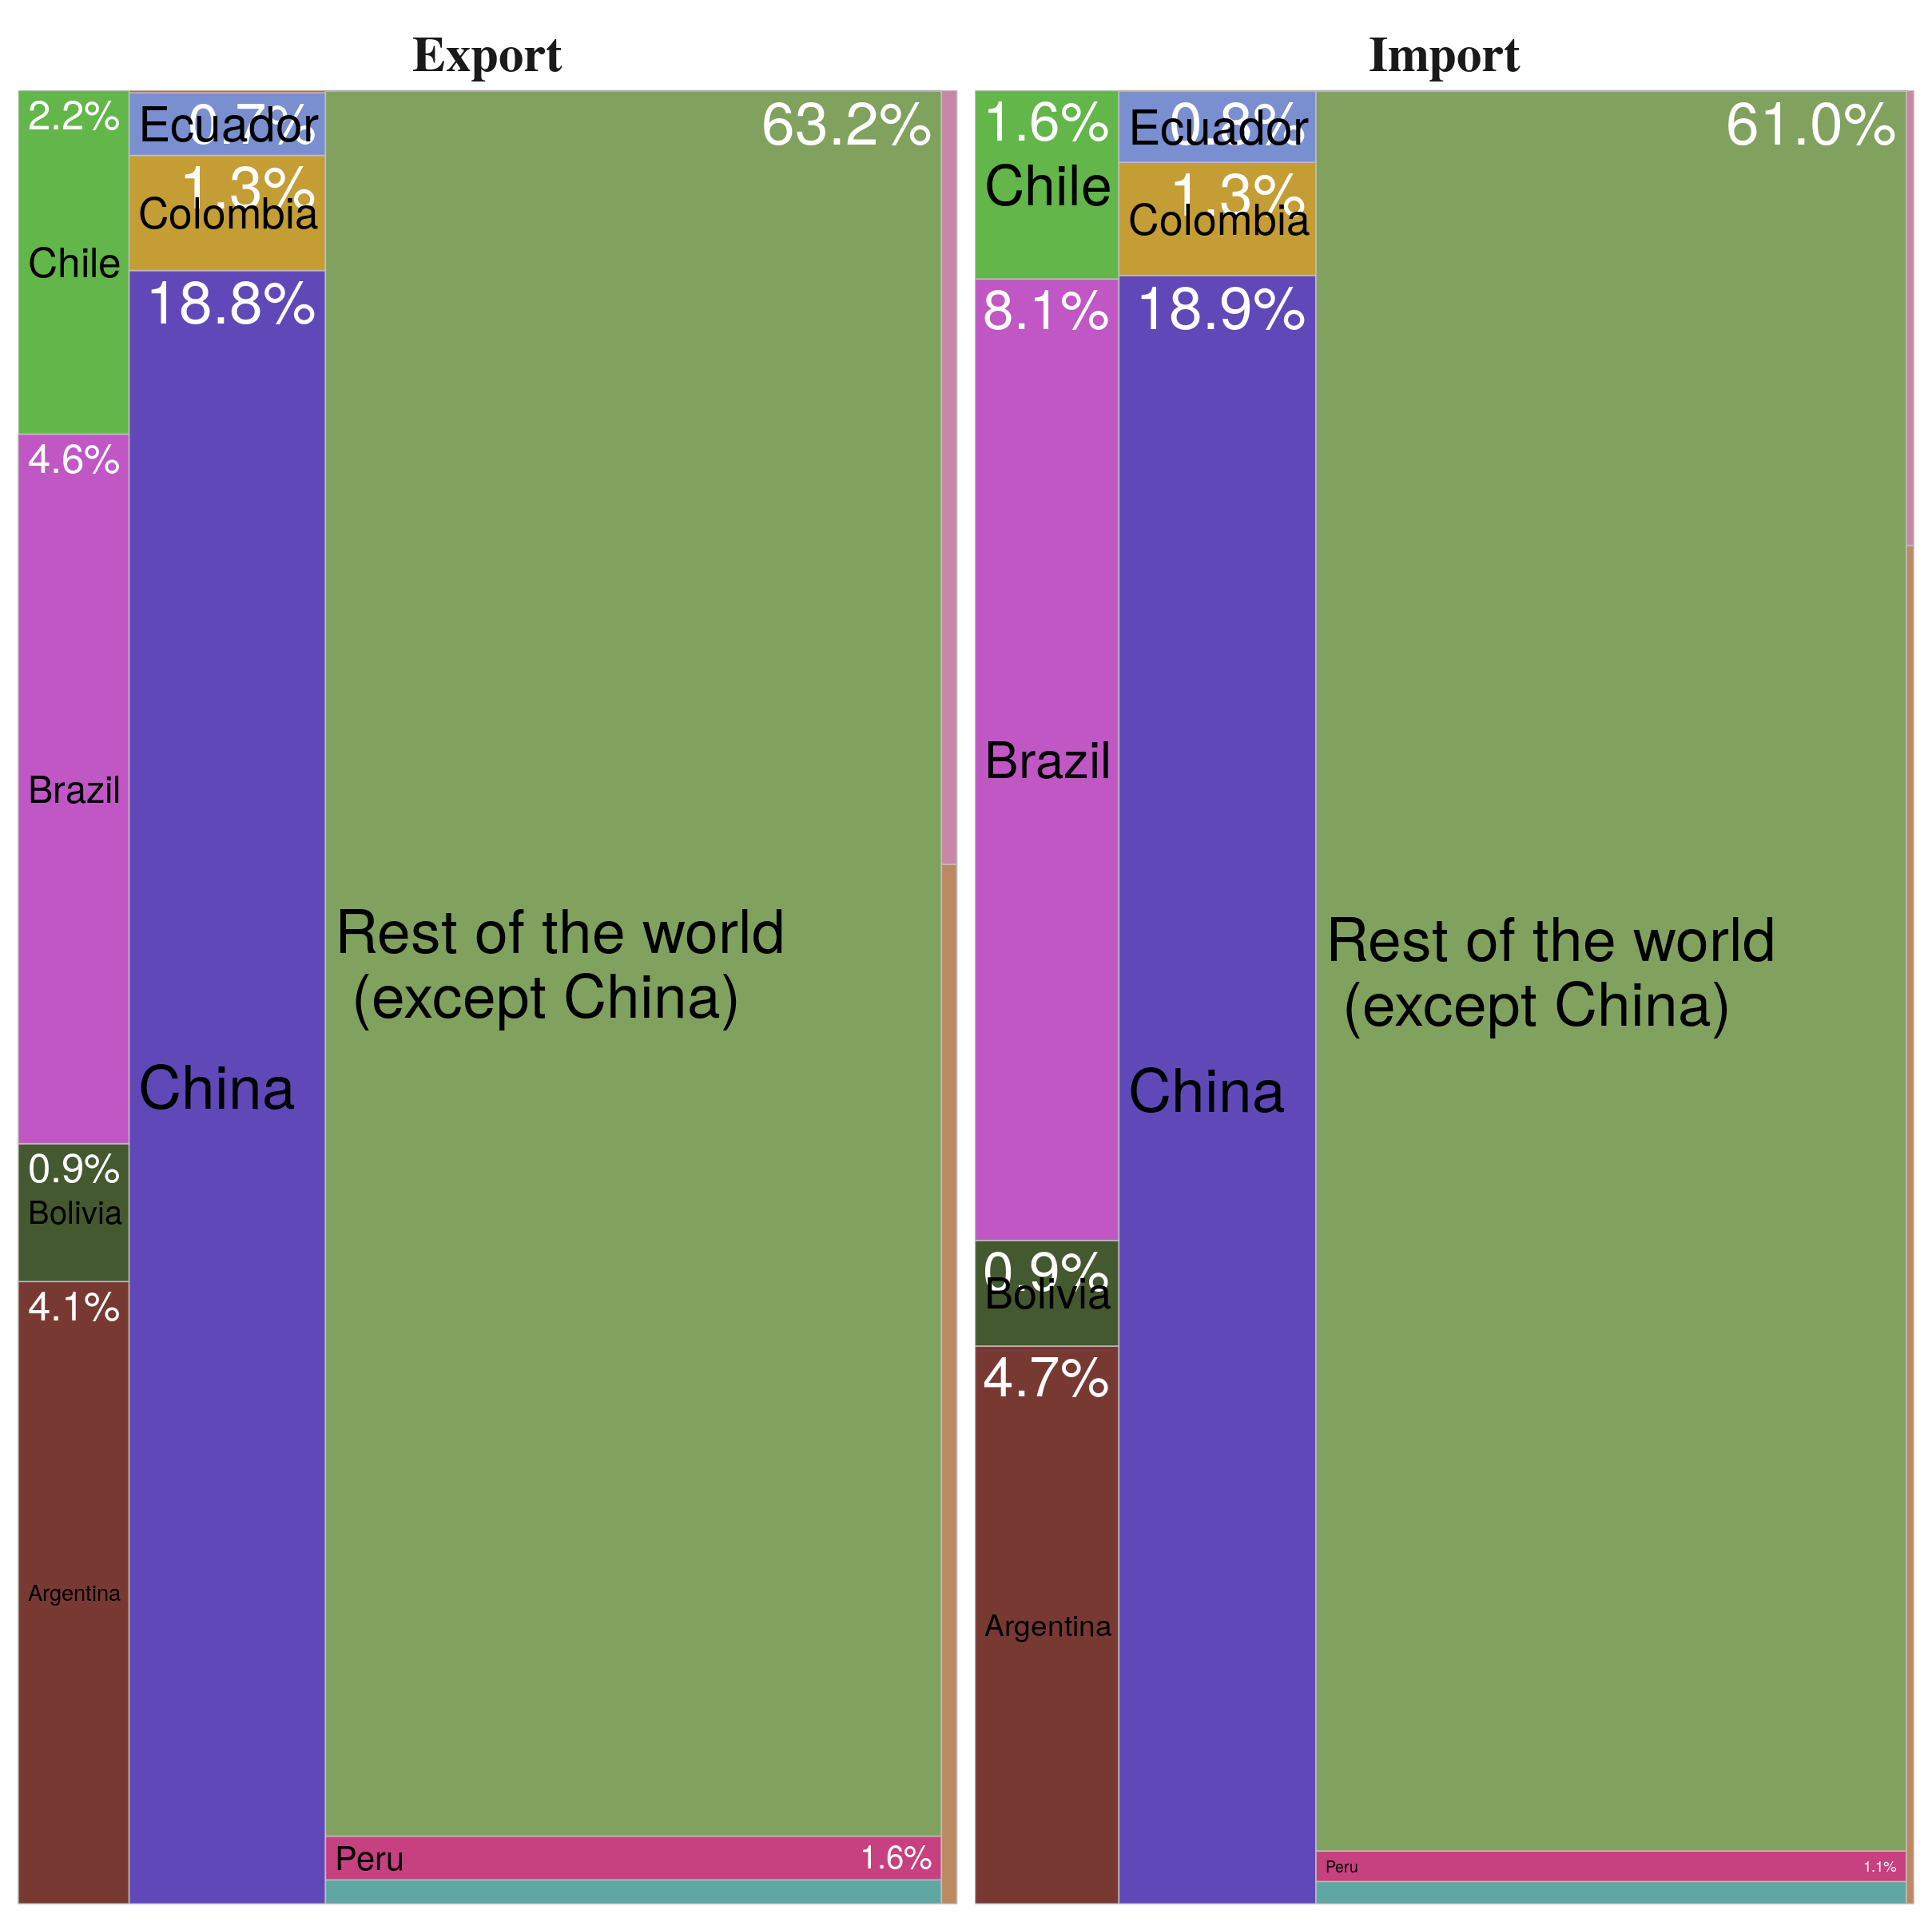
\includegraphics[width=.65\linewidth]{treemaps_paises_rdm2016}}
	\caption{Treemaps según socio comercial. 2016. Total Latinoamérica}
	\label{fig:treemaps_sudamerica_destino}
\end{figure}
	

De las figuras \ref{fig:treemaps_sudamerica_cadsubcad}, \ref{fig:treemaps_sudamerica_usos} y \ref{fig:treemaps_sudamerica_destino} se desprende que la región de Sudamérica tiene una baja integración regional en tanto una pequeña proporción de su comercio se realiza entre países de la región. A su vez, mientras el comercio intrarregional se realiza fundamentalmente sobre productos de alta complejidad y valor agregado, el comercio con el resto del mundo se encuentra desbalanceado: mientras las exportaciones se concentran en productos primarios de baja complejidad, aquellos productos que llegan desde el resto del mundo tienen un mayor grado de tecnificación. Estas conclusiones son particularmente válidas para el comercio con China, que constituye una quinta parte del comercio total de la región. Vale mencionar que la importancia de dicho país ah crecido de forma sostenida en el período analizado, siendo que en 1996 representaba menos de 2\% del comercio \footnote{ver \hyperlink{https://treemaps.shinyapps.io/treemaps/}{https://treemaps.shinyapps.io/treemaps/}}

\section{Metodología}

Del análisis exploratorio se desprende el potencial de la información desagregada a nivel producto para caracterizar la inserción en el mercado mundial de un país o región. Sin embargo, dada la alta cardinalidad de la información y la múltiples dimensiones de estudio, resulta dificultoso su estudio de forma general, sin hacer eje en un determinado país, o sin agregar la información según un nomenclador. En particular, el uso de agrupaciones jerárquicas de los productos resulta esencial para el análisis de resultados. La elaboración de los mismos constituye una extensa tarea por parte de expertos en las temáticas sectoriales de los diferentes tipos de productos, y el nomenclador resultante esta fuertemente determinado por los objetivos con que sera utilizado. Es por ello que en la presente sección se propone una elaboración alternativa de niveles jerárquicos de agrupamiento de productos. 

\info{agregar grafo bipartito}

	
\subsection{Latent Dirichlet Allocation Models}
	
El objetivo de la presente sección es elaborar un agrupamiento automático de los productos, basado en la información disponible. Este problema puede ser concebido desde dos puntos de vista: por un lado, se puede pensar como un problema de \textit{clustering} donde lo que se busca es crear grupos de productos con similares características. Por otro lado, es un problema de reducción de dimensionalidad, donde lo que se busca es encontrar un espacio de menor dimensión al que existen originalmente los datos. Esto sería posible dado que existe la posibilidad de explotar las similitudes y diferencias entre los distintos productos. 

Sin embargo, las técnicas de clustering tradicionales encuentran problemas en espacios de alta dimensionalidad \citep{aggarwal2001surprising}. A su vez, siguiendo el trabajo de \cite{molinari2016especializacion}, se entiende que los grupos no deberían ser excluyentes, dado que un mismo producto puede ser utilizado en diferentes formas, como producto intermedio o final. En este sentido, el problema se puede especificar como de \textit{clustering difuso}.
	
En concreto, la dimensionalidad del problema se puede pensar como el siguiente espacio:

$$
\mathcal{R}^{N*P*Y*2}
$$
Es decir la interacción de $N$ países, $P$ productos, $Y$ años, tanto para las exportaciones como las importaciones.
La propuesta es utilizar la técnica propuesta por \cite{blei2003latent} conocida como \textit{Latent Dirichlet Allocation Models} o \textit{Topic Modeling}. En su versión original, está técnica se propone como una forma de encontrar los tópicos presentes en un corpus, y la distribución de dichos tópicos sobre cada texto. Este problema es análogo al que se busca en el presente trabajo: Allí se busca una dimensión latente de $k$ tópicos, embebidos en un diccionario de alta dimensionalidad (las palabras presentes en el corpus), que se distribuyen a lo largo de los textos que componen dicho corpus. En el presente problema, se busca una dimensión latente de $k$ \textit{componentes}, embebidos en un nomenclador de alta dimensionalidad, que se distribuyen a lo largo de los países. Esta técnica a su vez puede ser pensada como un problema de clustering difuso, en tanto cada palabra (en el contexto original) puede pertenecer a más de un tópico.

A continuación se realizará una descripción del modelo propuesto por \cite{blei2003latent}, adaptado al presente dominio. 
	
\subsubsection{Definiciones}

\begin{itemize}
\item
Un \textbf{\emph{producto}} es la \emph{unidad básica discreta de los
	datos}, se define como un ítem de un nomenclador (SITC). Se representa
como un vector unitario. Definimos el superíndice \(i\) del vector
como el i-ésimo producto del nomenclador y el i-ésimo elemento del
vector. El V-ésimo producto del nomenclador es el vector \(w\), tal
que \(w^v\)=1 y \(w^u\)=0, \(u\neq v\)
\item
Un \textbf{\emph{país\&año}} es una secuencia de \textbf{N} productos,
definido como \(W= (w_1, w_2, ..., w_N)\)
\item
Nuestro \textbf{corpus} es la colección de \textbf{M} países, definido
como \(D = (d_1, d_2,..., d_M)\)
\item
Un \textbf{\emph{componente}} es una dimensión latente sobre el
corpus, y suponemos una cantidad fija \emph{k} de los mismos.
\item
Nuestro objetivo es obtener:
\end{itemize}

\begin{enumerate}
\def\labelenumi{\arabic{enumi}.}
\item
Una distribución de componentes sobre cada país\&año.
\item
Una distribución de los productos sobre los componentes.
\end{enumerate}


\subsubsection{Proceso generativo e inferencial}

Intuitivamente, suponemos el siguiente proceso generativo de datos:

\begin{itemize}
\item
Para cada país del corpus, imaginamos que las exportaciones surgen de
un proceso de dos etapas:

\begin{itemize}
	\item
	Elegimos aleatoriamente una distribución sobre los componentes
	\item
	Para cada dólar exportado:
	
	\begin{itemize}
		\item
		Elegimos aleatoriamente el componente al que pertence, dada la
		distribución definida en el paso anterior
		\item
		Elegimos aleatoriamente un producto de la distribución
		correspondiente a dicho componente
	\end{itemize}
\end{itemize}
\end{itemize}

\begin{enumerate}
\def\labelenumi{\arabic{enumi}.}
\item
Para cada Componente $k \in \{1,2,... K\}$
\end{enumerate}

\begin{itemize}
\item
Generar una distribución sobre los componentes
$\beta \sim Dir_v(\eta)$ con $\eta \in \mathcal{R}_{>0}$ un
parámetro fijo
\end{itemize}

\begin{enumerate}
\def\labelenumi{\arabic{enumi}.}
\setcounter{enumi}{1}
\item
Para cada país $d \in \{1,2,... D\}$
\end{enumerate}

\begin{itemize}
\item
generar un vector de proporciones de componentes
$\theta_d \sim Dir_K(\alpha)$ con $\alpha \in \mathcal{R}_{>0}^K$
un parámetro fijo
\item
Para cada dólar exportado:

\begin{enumerate}
	\def\labelenumi{\roman{enumi}.}
	\item
	generar una asignación del componente $z_{dn} \sim Mult(\theta_d)$
	\item
	asignar el producto $w_{dn} \sim Mult(\beta_{zn})$
\end{enumerate}
\end{itemize}

En la figura \ref{fig:grafo_blei} se puede observar el proceso generativo de forma gráfica. Aquí, cada nodo representa una distribución de probabilidad. Las aristas significan que la distribución de salida definen los parámetros de la distribución de entrada. Los recuadros significan replicación: El recuadro interior representa que el proceso se realiza para cada dólar exportado en el país. El recuadro exterior representa que el proceso se realiza para cada
país en el corpus.


\begin{figure}
	\centering	
%	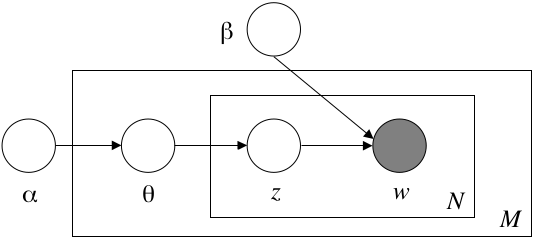
\includegraphics[width=.65\linewidth]{grafo}


\tikzset{every picture/.style={line width=0.75pt}} %set default line width to 0.75pt        

\begin{tikzpicture}[x=0.75pt,y=0.75pt,yscale=-1,xscale=1]
%uncomment if require: \path (0,300); %set diagram left start at 0, and has height of 300


%Shape: Circle [id:dp8853764007735601] 
\draw   (100,146) .. controls (100,132.19) and (111.19,121) .. (125,121) .. controls (138.81,121) and (150,132.19) .. (150,146) .. controls (150,159.81) and (138.81,171) .. (125,171) .. controls (111.19,171) and (100,159.81) .. (100,146) -- cycle ;
%Shape: Circle [id:dp33419535302461556] 
\draw   (205,146) .. controls (205,132.19) and (216.19,121) .. (230,121) .. controls (243.81,121) and (255,132.19) .. (255,146) .. controls (255,159.81) and (243.81,171) .. (230,171) .. controls (216.19,171) and (205,159.81) .. (205,146) -- cycle ;
%Shape: Circle [id:dp6232220468757862] 
\draw   (281,47) .. controls (281,33.19) and (292.19,22) .. (306,22) .. controls (319.81,22) and (331,33.19) .. (331,47) .. controls (331,60.81) and (319.81,72) .. (306,72) .. controls (292.19,72) and (281,60.81) .. (281,47) -- cycle ;
%Shape: Circle [id:dp49572645552205263] 
\draw  [fill={rgb, 255:red, 199; green, 199; blue, 199 }  ,fill opacity=1 ] (410,145) .. controls (410,131.19) and (421.19,120) .. (435,120) .. controls (448.81,120) and (460,131.19) .. (460,145) .. controls (460,158.81) and (448.81,170) .. (435,170) .. controls (421.19,170) and (410,158.81) .. (410,145) -- cycle ;
%Shape: Circle [id:dp04424520000997234] 
\draw   (311,145) .. controls (311,131.19) and (322.19,120) .. (336,120) .. controls (349.81,120) and (361,131.19) .. (361,145) .. controls (361,158.81) and (349.81,170) .. (336,170) .. controls (322.19,170) and (311,158.81) .. (311,145) -- cycle ;
%Shape: Rectangle [id:dp8518034256278205] 
\draw   (299.13,100.76) -- (496.19,100.76) -- (496.19,199.76) -- (299.13,199.76) -- cycle ;
%Shape: Rectangle [id:dp2099791938650164] 
\draw   (173,86) -- (515.13,86) -- (515.13,221.72) -- (173,221.72) -- cycle ;
%Straight Lines [id:da11406541597292297] 
\draw    (150,146) -- (203,146) ;
\draw [shift={(205,146)}, rotate = 180] [fill={rgb, 255:red, 0; green, 0; blue, 0 }  ][line width=0.75]  [draw opacity=0] (8.93,-4.29) -- (0,0) -- (8.93,4.29) -- cycle    ;

%Straight Lines [id:da3621589464216769] 
\draw    (255,146) -- (309,145.04) ;
\draw [shift={(311,145)}, rotate = 538.98] [fill={rgb, 255:red, 0; green, 0; blue, 0 }  ][line width=0.75]  [draw opacity=0] (8.93,-4.29) -- (0,0) -- (8.93,4.29) -- cycle    ;

%Straight Lines [id:da09879567766811748] 
\draw    (361,145) -- (408,145) ;
\draw [shift={(410,145)}, rotate = 180] [fill={rgb, 255:red, 0; green, 0; blue, 0 }  ][line width=0.75]  [draw opacity=0] (8.93,-4.29) -- (0,0) -- (8.93,4.29) -- cycle    ;

%Straight Lines [id:da23517788835593556] 
\draw    (328.92,60.5) -- (413.33,125.45) ;
\draw [shift={(414.92,126.67)}, rotate = 217.57] [fill={rgb, 255:red, 0; green, 0; blue, 0 }  ][line width=0.75]  [draw opacity=0] (8.93,-4.29) -- (0,0) -- (8.93,4.29) -- cycle    ;


% Text Node
\draw (125,178) node  [align=left] {$\displaystyle \alpha $};
% Text Node
\draw (227.58,179) node  [align=left] {$\displaystyle \theta $};
% Text Node
\draw (338.42,177) node  [align=left] {$\displaystyle z$};
% Text Node
\draw (437.42,177) node  [align=left] {$\displaystyle w$};
% Text Node
\draw (270,44) node  [align=left] {$\displaystyle \beta $};
% Text Node
\draw (484,189) node  [align=left] {$\displaystyle N$};
% Text Node
\draw (504,208) node  [align=left] {$\displaystyle M$};


\end{tikzpicture}

	\caption{fuente: \cite{blei2003latent}}
	\label{fig:grafo_blei}
\end{figure}



Un Proceso de Dirichlet es una familia de procesos estocásticos donde las realizaciones son ellas mismas distribuciones de probabilidad. Es decir, el rango de esta distribución (así como en una normal son los reales) son distribuciones de probabilidad. Para interpretarlo geométricamente, la figura \ref{fig:dirichlet} muestra un ejemplo de la distribución de densidad para 3 productos y 4 componentes. El triángulo representa todas las distribuciones (multinomiales)
posibles sobre los tres productos. Cada uno de los vértices del triángulo es una distribución de probabilidad que asigna una probabilidad de 1 a uno de los productos. El punto medio de cada lado, es una distribución con probabilidad 0.5 a dos componentes. El cuarto componente, el centroide del triángulo, asigna probabilidad de $\frac{1}{3}$ a cada producto. Los cuatro puntos marcado con x son las distribuciones multinomiales de $p(w|z)$  para cada uno de los cuatro componentes. La altura en el eje z es una posible distribución de densidad sobre el
simplex, es decir, sobre las distribuciones de densidad multinomiales, dada por LDA.

\begin{figure}
	\centering	
	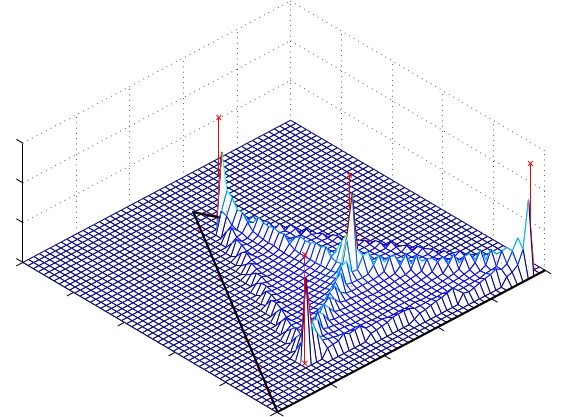
\includegraphics[width=.65\linewidth]{dirichlet}
	\caption{fuente: \cite{blei2003latent}}
	\label{fig:dirichlet}
\end{figure}

Cuando observamos los datos, no contamos con los tópicos ni con su
distribución, sino con los productos y países. El objetivo es realizar
inferencia sobre las variables latentes, mediante el Teorema de Bayes:

$$
p(\theta,z|w,\alpha,\beta) = \frac{p(\theta,z,w|\alpha,\beta)}{p(w|\alpha,\beta)}
$$

Nuestra función objetivo es:

$$
\ell(\alpha, \beta) = \sum_{d=1}^M \log p(w_d|\alpha,\beta)
$$

El problema es que esta ecuación es intratable, por la interacción entre $\theta$ y $\beta$. Por ello, la inferencia se realiza sobre una familia de modelos que se sabe que son una cota inferior de probabilidad, y que son tratables. Estos modelos tienen parámetros variacionales, que se ajustan para obtener el modelo que más se acerca a la cota inferior. La forma de obtener una familia de modelos tratables es considerar algunas modificaciones sobre el modelo gráfico original, removiendo nodos y aristas \citep{hoffman2013stochastic}. En la figura \ref{fig:grafo_variational} se puede observar la solución propuesta por \citep{blei2003latent} que, dado que utilizamos la implementación del modelo que se encuentra en \cite{scikit-learn} es también la del presente trabajo.

\begin{figure}[h]
	\centering	
%	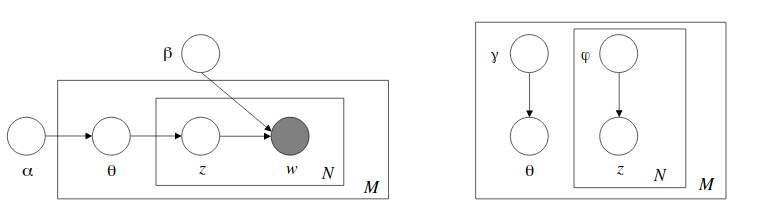
\includegraphics[width=.65\linewidth]{grafo_variational}



\tikzset{every picture/.style={line width=0.75pt}} %set default line width to 0.75pt        

\begin{tikzpicture}[x=0.4pt,y=0.4pt,yscale=-1,xscale=1]
%uncomment if require: \path (0,300); %set diagram left start at 0, and has height of 300

%Shape: Circle [id:dp8853764007735601] 
\draw   (14,151) .. controls (14,137.19) and (25.19,126) .. (39,126) .. controls (52.81,126) and (64,137.19) .. (64,151) .. controls (64,164.81) and (52.81,176) .. (39,176) .. controls (25.19,176) and (14,164.81) .. (14,151) -- cycle ;
%Shape: Circle [id:dp33419535302461556] 
\draw   (119,151) .. controls (119,137.19) and (130.19,126) .. (144,126) .. controls (157.81,126) and (169,137.19) .. (169,151) .. controls (169,164.81) and (157.81,176) .. (144,176) .. controls (130.19,176) and (119,164.81) .. (119,151) -- cycle ;
%Shape: Circle [id:dp6232220468757862] 
\draw   (195,52) .. controls (195,38.19) and (206.19,27) .. (220,27) .. controls (233.81,27) and (245,38.19) .. (245,52) .. controls (245,65.81) and (233.81,77) .. (220,77) .. controls (206.19,77) and (195,65.81) .. (195,52) -- cycle ;
%Shape: Circle [id:dp49572645552205263] 
\draw  [fill={rgb, 255:red, 199; green, 199; blue, 199 }  ,fill opacity=1 ] (324,150) .. controls (324,136.19) and (335.19,125) .. (349,125) .. controls (362.81,125) and (374,136.19) .. (374,150) .. controls (374,163.81) and (362.81,175) .. (349,175) .. controls (335.19,175) and (324,163.81) .. (324,150) -- cycle ;
%Shape: Circle [id:dp04424520000997234] 
\draw   (225,150) .. controls (225,136.19) and (236.19,125) .. (250,125) .. controls (263.81,125) and (275,136.19) .. (275,150) .. controls (275,163.81) and (263.81,175) .. (250,175) .. controls (236.19,175) and (225,163.81) .. (225,150) -- cycle ;
%Shape: Rectangle [id:dp8518034256278205] 
\draw   (213.13,105.76) -- (411.6,105.76) -- (411.6,208) -- (213.13,208) -- cycle ;
%Shape: Rectangle [id:dp2099791938650164] 
\draw   (87,91) -- (440.6,91) -- (440.6,233) -- (87,233) -- cycle ;
%Straight Lines [id:da11406541597292297] 
\draw    (64,151) -- (117,151) ;
\draw [shift={(119,151)}, rotate = 180] [fill={rgb, 255:red, 0; green, 0; blue, 0 }  ][line width=0.75]  [draw opacity=0] (8.93,-4.29) -- (0,0) -- (8.93,4.29) -- cycle    ;

%Straight Lines [id:da3621589464216769] 
\draw    (169,151) -- (223,150.04) ;
\draw [shift={(225,150)}, rotate = 538.98] [fill={rgb, 255:red, 0; green, 0; blue, 0 }  ][line width=0.75]  [draw opacity=0] (8.93,-4.29) -- (0,0) -- (8.93,4.29) -- cycle    ;

%Straight Lines [id:da09879567766811748] 
\draw    (275,150) -- (322,150) ;
\draw [shift={(324,150)}, rotate = 180] [fill={rgb, 255:red, 0; green, 0; blue, 0 }  ][line width=0.75]  [draw opacity=0] (8.93,-4.29) -- (0,0) -- (8.93,4.29) -- cycle    ;

%Straight Lines [id:da23517788835593556] 
\draw    (242.92,65.5) -- (327.33,130.45) ;
\draw [shift={(328.92,131.67)}, rotate = 217.57] [fill={rgb, 255:red, 0; green, 0; blue, 0 }  ][line width=0.75]  [draw opacity=0] (8.93,-4.29) -- (0,0) -- (8.93,4.29) -- cycle    ;

%Shape: Rectangle [id:dp7501348302770449] 
\draw   (701,53.33) -- (803,53.33) -- (803,222.33) -- (701,222.33) -- cycle ;
%Shape: Rectangle [id:dp832082779713454] 
\draw   (551,46.33) -- (841,46.33) -- (841,237.33) -- (551,237.33) -- cycle ;
%Shape: Circle [id:dp8534167348661814] 
\draw   (610.39,157.5) .. controls (624.2,157.56) and (635.34,168.8) .. (635.28,182.61) .. controls (635.22,196.42) and (623.98,207.56) .. (610.17,207.5) .. controls (596.37,207.44) and (585.22,196.2) .. (585.28,182.39) .. controls (585.34,168.58) and (596.59,157.44) .. (610.39,157.5) -- cycle ;
%Shape: Circle [id:dp4466934905564389] 
\draw   (610.83,58.5) .. controls (624.63,58.56) and (635.78,69.8) .. (635.72,83.61) .. controls (635.66,97.42) and (624.41,108.56) .. (610.61,108.5) .. controls (596.8,108.44) and (585.66,97.2) .. (585.72,83.39) .. controls (585.78,69.58) and (597.02,58.44) .. (610.83,58.5) -- cycle ;
%Straight Lines [id:da2762808842403305] 
\draw    (610.61,108.5) -- (610.4,155.5) ;
\draw [shift={(610.39,157.5)}, rotate = 270.25] [fill={rgb, 255:red, 0; green, 0; blue, 0 }  ][line width=0.75]  [draw opacity=0] (8.93,-4.29) -- (0,0) -- (8.93,4.29) -- cycle    ;

%Shape: Circle [id:dp49555163496653243] 
\draw   (753.39,158.5) .. controls (767.2,158.56) and (778.34,169.8) .. (778.28,183.61) .. controls (778.22,197.42) and (766.98,208.56) .. (753.17,208.5) .. controls (739.37,208.44) and (728.22,197.2) .. (728.28,183.39) .. controls (728.34,169.58) and (739.59,158.44) .. (753.39,158.5) -- cycle ;
%Shape: Circle [id:dp6912113806172252] 
\draw   (753.83,59.5) .. controls (767.63,59.56) and (778.78,70.8) .. (778.72,84.61) .. controls (778.66,98.42) and (767.41,109.56) .. (753.61,109.5) .. controls (739.8,109.44) and (728.66,98.2) .. (728.72,84.39) .. controls (728.78,70.58) and (740.02,59.44) .. (753.83,59.5) -- cycle ;
%Straight Lines [id:da3696244463925229] 
\draw    (753.61,109.5) -- (753.4,156.5) ;
\draw [shift={(753.39,158.5)}, rotate = 270.25] [fill={rgb, 255:red, 0; green, 0; blue, 0 }  ][line width=0.75]  [draw opacity=0] (8.93,-4.29) -- (0,0) -- (8.93,4.29) -- cycle    ;


% Text Node
\draw (39,189) node  [align=left] {$\displaystyle \alpha $};
% Text Node
\draw (142.58,190) node  [align=left] {$\displaystyle \theta $};
% Text Node
\draw (252.42,188) node  [align=left] {$\displaystyle z$};
% Text Node
\draw (351.42,188) node  [align=left] {$\displaystyle w$};
% Text Node
\draw (184,49) node  [align=left] {$\displaystyle \beta $};
% Text Node
\draw (398,194) node  [align=left] {$\displaystyle N$};
% Text Node
\draw (423,217) node  [align=left] {$\displaystyle M$};
% Text Node
\draw (788,209) node  [align=left] {$\displaystyle N$};
% Text Node
\draw (825,222) node  [align=left] {$\displaystyle M$};
% Text Node
\draw (570.58,183) node  [align=left] {$\displaystyle \theta $};
% Text Node
\draw (569.58,81) node  [align=left] {$\displaystyle \gamma $};
% Text Node
\draw (713.58,82) node  [align=left] {$\displaystyle \varphi $};
% Text Node
\draw (714.42,181) node  [align=left] {$\displaystyle z$};


\end{tikzpicture}

	\caption{fuente: \cite{blei2003latent}}
	\label{fig:grafo_variational}
\end{figure}


La estimación de los parámetros se realiza a través del proceso de \emph{variational Expectation Maximization} (EM):

\begin{itemize}
\item \textbf{paso E}: Optimizamos los parámetros variacionales $\gamma, \varphi$
\item \textbf{paso M}: Para los valores fijos $\gamma, \varphi$, maximizamos la cota inferior respecto a los parámetros del modelo, $\alpha,\beta$
\end{itemize}

Estos dos pasos se alternan hasta converger. Por último, se realiza un suavizado sobre las probabilidades que un componente asigna a un producto, para que sean siempre mayores a 0.



\subsection{Grafo Bipartito}

Otra manera de analizar el comercio internacional considerando la dimensión \textit{producto} es mediante técnicas de análisis de redes. Es difundido en la literatura el uso de grafos bipartitos para este análisis \citep{10.1371/journal.pone.0197575,straka2017grand,ferreira2016topology,caldarelli2012network}. En la figura \ref{fig:bipgraph} se puede observar un diagrama de un grafo bipartito de países, \textit{a}, y productos, \textit{b}. Una arista entre un país $a_c$ y un producto $b_i$ representa en este caso que el país $a_c$ exporta el producto $b_i$. Dado que tanto los países como los productos se representan como nodos, la estructura de grafo bipartito nos permite mantener la diferencia cualitativa entre ambos tipos de vértices.


\begin{figure}
	\centering
\begin{tikzpicture}

\begin{scope}[rotate=90]
\SetVertexMath
\grEmptyLadder[RA=1,RB=2]{4}   
\end{scope}
\Edges(b2,a0,b0,a1,b2,a3,b1,a2)
\end{tikzpicture} 

\caption{Grafo bipartito, países y productos} \label{fig:bipgraph}
\end{figure}


Tal como sucedía con el comercio agregado a nivel países, los tamaños relativos de las economías nacionales implican que un mismo monto exportado tenga un significado muy distinto según el país del cual provienen. A su vez, como los volúmenes comerciados de los diferentes productos también varían fuertemente, lo anterior aplica a este otro tipo de nodos. Es por ello que en la literatura se utiliza una normalización de las exportaciones, conocida como \textit{Ventajas Comparativas Relativas}, o \textit{RCA} por sus siglas en inglés. La misma fue propuesta por \cite{balassa1965trade} y tiene la siguiente forma funcional:

$$
\operatorname{RCA}(c, i)= \frac{\displaystyle \frac{x(c, i)}{\sum_{i} x(c, i)}}{\displaystyle \frac{\sum_{c} x(c, i)}{\sum_{c, i} x(c, i)}}
$$

Dónde $x(c,i)$ es el valor de las exportaciones del \textit{país c} en \textit{producto i}. El numerador indica la proporción que dicho producto representa en las exportaciones totales del país c. El denominador indica la proporción que este mismo producto representa en las exportaciones totales de todos los países. Es decir, \textit{RCA} muestra la relación en la importancia de un producto $i$ en un país $c$ respecto de la importancia promedio de ese producto en la economía mundial. De esta forma, un RCA alto implica que el país en cuestión tiene \textit{ventaja relativa} para exportar un producto, mientras que un RCA bajo implica que el país tiene una \textit{desventaja relativa} con el producto. De esta forma, se puede construir un grafo no ponderado estableciendo el punto de corte en $RCA>1$. 

Habiendo establecido nodos y aristas del grafo bipartito, el problema reside en que la mayor parte de las técnicas de análisis sobre grafos están definidas para grafos simples, no para grafos bipartitos. Por ello se continúa por realizar la proyección sobre uno de los tipos de nodos para luego analizar los resultados \citep{zhou2007bipartite}. La proyección se realiza de forma ponderada y el peso asignado a una arista entre dos nodos es la cantidad de nodos del otro tipo con los cuales estaban conectados ambos nodos en el grafo original. Esto significa, en la proyección del grafo de países, que aquellos que compartían ventajas comparativas relativas sobre un conjunto grande productos estarán fuertemente conectados, mientras que los países que poseen canastas exportadoras muy diferentes, estarán débilmente conectados.

Este procedimiento se realizó para los nodos-país. El resultados es un grafo de características similares al elaborado en el capítulo anterior, pero que en esta oportunidad los vínculos entre países no reflejan sus vínculos comerciales, sino su similitud respecto a la estructura productiva exportadora. A diferencia del grafo de relaciones comerciales, aquí las métricas de centralidad no resultan particularmente interesantes porque el centro del grafo esta poblado por aquellos países que exportan las mercancías más comunes, mientras que en los márgenes se encuentran aquellos cuya canasta exportadora resulta muy diferente a la media. Lo que resulta particularmente interesante son las comunidades que se generan en el grafo, para ver si las mismas tienen alguna relación con lo dicho en la literatura respecto de la Nueva División Internacional del Trabajo \citep{frobel1978new}. Para ello se utilizaron técnicas de detección de comunidades. En particular, se utilizo el \textit{clustering de Louvain} \citep{blondel2008fast},donde se optimiza la modularidad de los clusters de forma \textit{greedy}. También se utilizó el método de detección de comunidades \textit{Walktrap} \citep{pons2005computing}, que se basa en la noción de que al realizar \textit{random walks} en el grafo, estos caminos tienden a quedarse atrapados en las secciones más densas del grafo, que corresponden a las comunidades. En ambas técnicas en número de comunidades encontradas es definido de forma automática por el algoritmo. 

Para el análisis de los productos, nos basamos en el concepto de \textit{proximidad} de \cite{Hidalgo2009,Hidalgo2009a,Hidalgo2007} definido como:

$$
\phi_{ij} = min (P(RCA_i>1/RCA_j>1),P(RCA_j>1/RCA_i>1))
$$

dónde $P(RCA_i/RCA_j)$ es la probabilidad condicional de exportar el producto $i$ dado que exporta el producto $j$. Es decir:

$$
P(RCA_i >1 /RCA_j >1) = \frac{P(RCA_i >1 \cap RCA_j >1)}{P(RCA_j >1)}
$$

$$
\text{con } P(RCA_j >1)= \frac{ \sum_{c} I(RCA_c >1)}{N}
$$

siendo N la cantidad de países y $\sum_{c}$ la sumatoria en los países. Es decir, la proporción de países en los cuales el producto $j$ tiene un $RCA>1$. Por su parte: 

$$
P(RCA_i >1 \cap RCA_j >1) = \frac{\sum_c I(RCA_i >1) \cap I(RCA_j >1)}{N}
$$

Esto es, la probabilidad de que un país tenga para ambos productos ventajas comparativas relativas. Por lo tanto, $\phi_{ij}$ establece que dos productos son similares si son exportados por los mismos países. Dado que existen productos que son ubicuos, es decir que son exportados por la mayoría de los países, y son muchos quienes tienen un $RCA>1$, y que una métrica de distancia debe cumplir con el principio de simetría ($d(x,y)=d(y,x)$), esta función toma el mínimo de ambos valores. 


$\Phi$ es por lo tanto una matriz de distancias entre los productos. Esto resulta ideal para analizar los datos a través de la técnica de clustering \textit{K-medioids} \citep{kaufman1987clustering}. Este método construye K clusters de forma iterativa modificando el centro del cluster para optimizar la bondad de ajuste. A diferencia de K-means \citep{macqueen1967some} el centro de cada cluster se define en una observación existente en el dataset, y por lo tanto se puede recuperar a las mismas para caracterizar el cluster. En es caso del espacio de productos esto resulta de utilidad para comprender los grupos que se conforman. Finalmente, dado que se presentan los datos en un \textit{heatmap}, se decidió también utilizar la técnica de clustering jerárquico propuesta por \cite{ward1963hierarchical} para su ordenamiento.

\section{Resultados}

\subsection{Latent Dirichlet Allocation Models}

Los resultado obtenidos de los modelos de Topic Modelling para el análisis de textos normalmente se analizan en dos etapas: En primer lugar se etiquetan los tópicos obtenidos sobre la base de las palabras más salientes de cada tópico, y luego se analiza su distribución en los textos. El etiquetado de los tópicos es una tarea subjetiva donde lo que se busca es un concepto generalizador de aquellas palabras que componen al tópico, donde es posible que esta tarea no se pueda realizar por falta de coherencia dentro del tópico. El hiperparámero $k$, es decir la cantidad de tópicos, juega un rol fundamental en este punto, dado que con una cantidad baja de tópicos estos tenderán a reflejar conceptos amplios, mientras que si $k$ es mayor que la cardinalidad del espacio latente que se busca, esto puede generar tópicos repetidos. 
Lo anterior no escapa al presente dominio sino que se refuerza, dado que la búsqueda, subjetiva, de un concepto abarcador entre productos puede resultar más compleja que la de un concepto generalizador de un grupo de palabras. Un problema que no existe en el presente dominio es el de la polisemia, dado que todos los significantes, indices del nomenclador, hacen referencia a un único significado no ambiguo. Sin embargo, nuevos problemas aparecen respecto a este punto, como qué nomenclador de base utilizar y en qué nivel de desagregación. Por motivos de comparabilidad con los resultados de \cite{molinari2016especializacion} se decidió utilizar el nomenclador SITC a 4 dígitos \citep{un2006standard}. A su vez, se realizaron pruebas para varios valores de $k$: 2,4,6,8,10,20,30,40,50, 100 y 200. Para el etiquetado de los componentes se observó que la práctica usual de observar los primeros diez elementos de la distribución no bastaba para encontrar una etiqueta generalizadora, por lo que se elaboró un tablero dinámico para estudiar la distribución y su función acumulada, a la vez que se gráfico la distribución en función de un nomenclador de complejidad tecnológica \citep{lall2000technological}: 

\begin{table}
	\centering
	\begin{tabular}{ll}
		\hline
		 Código & Descripción \\ 
		\hline
		01 & Primary products \\ 
		02 & Resource-based manufactures: agro-based \\ 
		03 & Resource-based manufactures: other \\ 
		04 & Low technology manufactures: textile, garment and footwear \\ 
		05 & Low technology manufactures: other products \\ 
		06 & Medium technology manufactures: automotive \\ 
		07 & Medium technology manufactures: process \\ 
		08 & Medium technology manufactures: engineering \\ 
		09 & High technology manufactures: electronic and electrical \\ 
		10 & High technology manufactures: other \\ 
		99 & Unclassified products \\ 
		\hline
	\end{tabular}
\end{table}

En la figura \ref{fig:dist_40_4} se puede observar la tabla utilizada para caracterizar el cuarto componente en el modelo con $k=4$. Allí se observa que la mayoría de los componentes pertenecen al rubro textil, como pulloveres, remeras y pantalones. También se aparece el té, que no guarda coherencia con le resto del rubro.
\info{revisar}

\begin{figure}
	\centering	
	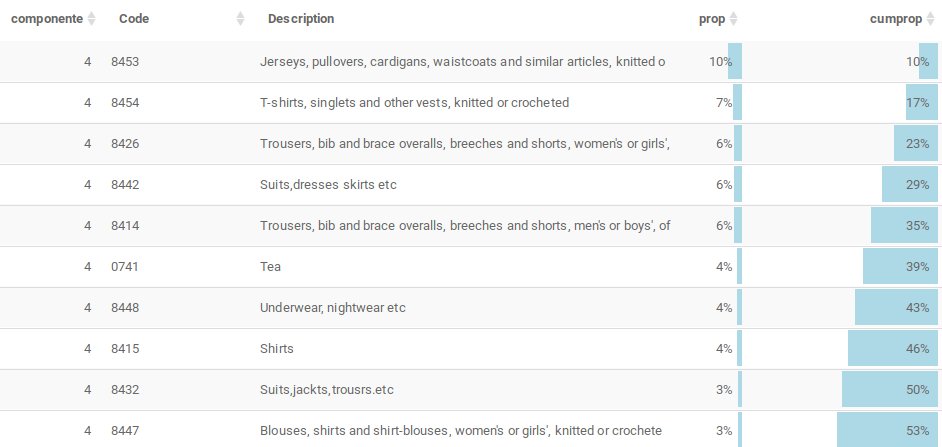
\includegraphics[width=\linewidth]{dist_40_4}
	\caption{Distribución del Componente 4. K = 40}
	\label{fig:dist_40_4}
\end{figure}

La figura muestra la distribución siguiendo los grupos de \cite{lall2000technological}. Aquí se puede confirmar que la distribución se concentra fuertemente en la categoría 4, textiles. 

\begin{figure}
	\centering	
	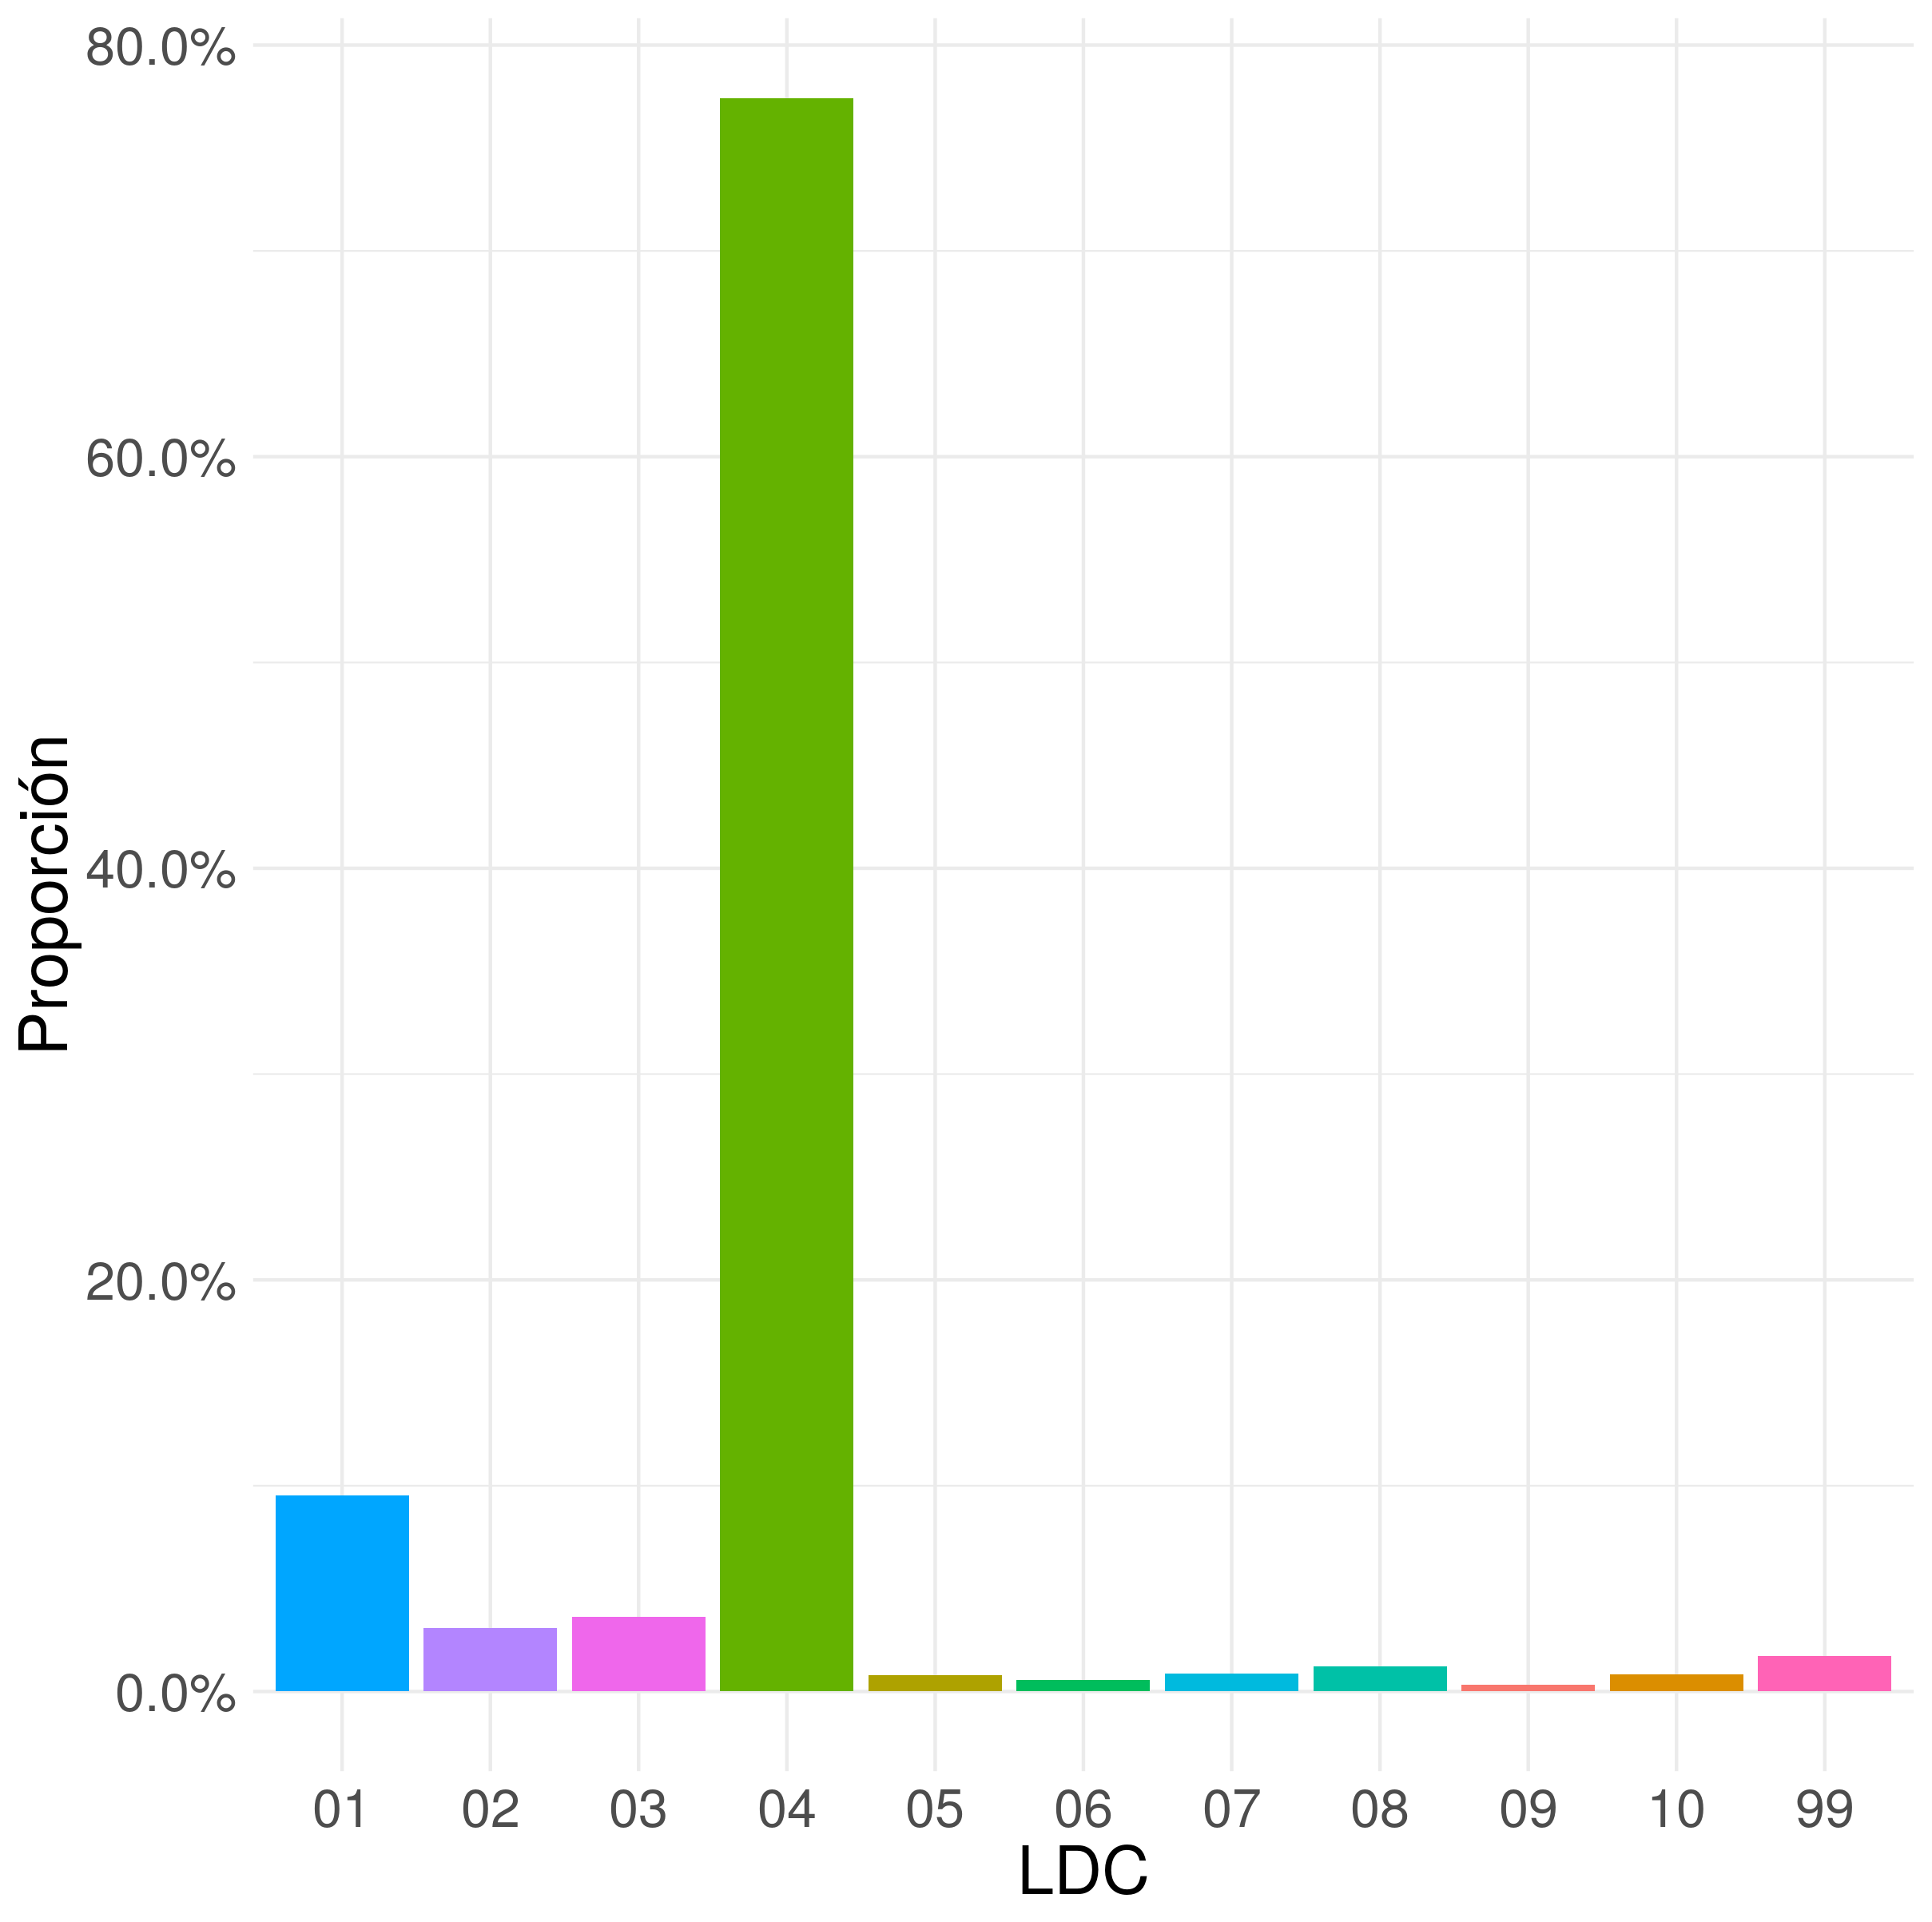
\includegraphics[width=0.65\linewidth]{graficoLall_k40_comp4}
	\caption{Distribución del Componente 4. K = 40 según Lall}
	\label{fig:dist_40_4_lall}
\end{figure}

una de las problemáticas observadas en el análisis de los diferentes ejercicios es definir la granularidad correcta del objeto de estudio. Como se mencionó arriba, el parámetro $k$ define cuan específicos o genéricos son los componentes obtenidos. El problema surge en que en el análisis económico aquellos fenómenos que resulta de interés explorar pueden encontrarse a diferentes niveles de granularidad. Esto es, desde el punto de vista económico puede resultar de interés seguir el comportamiento de un componente que refiera a \textit{derivados de la soja}, pero para poder dar con el mismo, sería necesario un nivel de granularidad que puede implicar que otro concepto interesante como \textit{productos textiles} se multiplique a lo largo de varios componentes. 

Por otro lado, la figura \ref{fig:componentes} muestra la distribución promedio de los componentes en los países, para varios valores de $k$. Se puede observar que el segundo componente siempre toma un valor elevado, por encima del 40\%, mientras que el resto de la distribución de distribuye de forma más o menos uniforme entre los restantes componentes. Esto se puede interpretar como que una proporción importante del comercio mundial se realiza en productos muy similares entre sí, en tanto los países que los exportan tienden a ser los mismos. Este \textit{componente gigante} del comercio no se fragmenta al aumentar $k$ dado que lo que sucede es que se subfragmenta el restante del comercio. 

\begin{figure}
	\centering	
	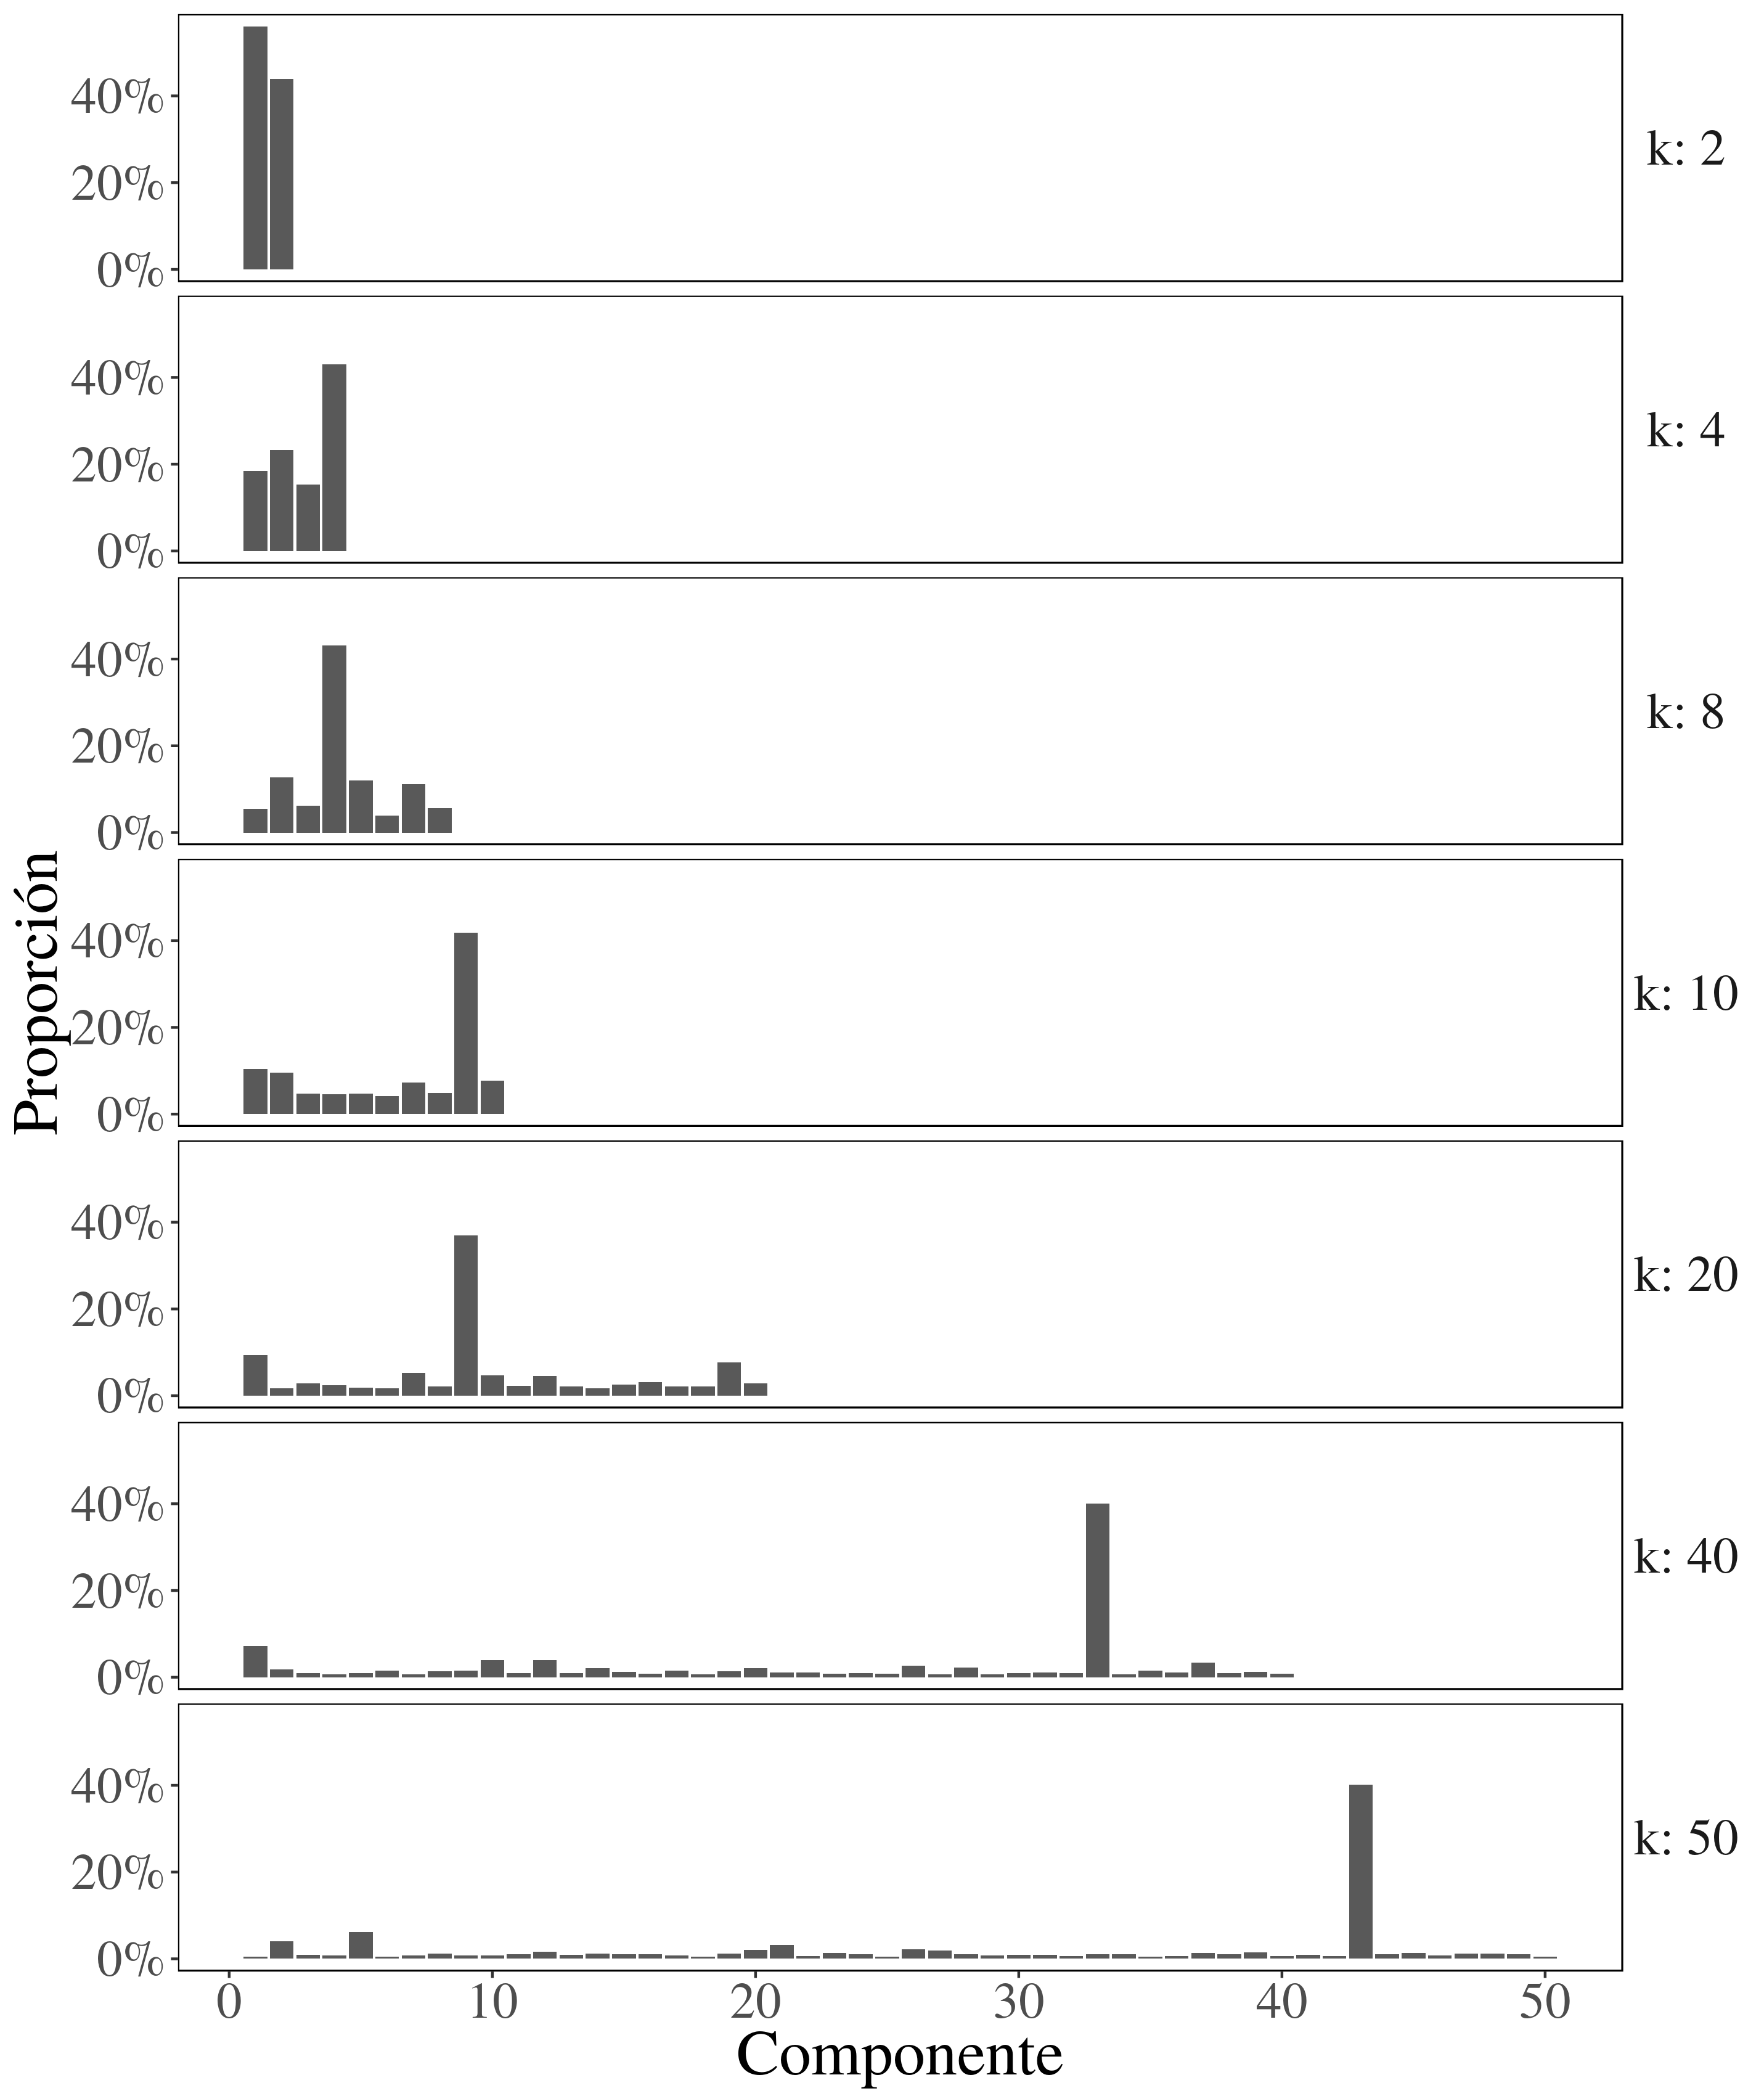
\includegraphics[width=0.65\linewidth]{componentes}
	\caption{Distribución promedio de los componentes en los países, varios valores de k}
	\label{fig:componentes}
\end{figure}

Esta conclusiones encuentran su correlato en la bibliografía. \cite{Hidalgo2007} construye un espacio de productos a partir de la proyección de un grafo bipartito de países y productos, y el resultado muestra evidencias de un núcleo densamente conectado y representativo respecto del comercio global. En este sentido, el $k$ óptimo es aquel que logra separar correctamente los clusters de productos que se encuentran en la periferia de dicho núcleo. Áreas como el \textit{petróleo}, \textit{textiles} y \textit{productos agropecuarios} deberían ser distinguibles con nitidez. Con este objetivo en mente, de los diferentes experimentos para diferentes valores del hiperparámetro, se concluyo que $k=40$ \info{rehacer}arroja los mejores resultados para este conjunto de datos.
\info{rehacer}
Finalmente, para elaborar las etiquetas finales se consultó especialistas sectoriales. En la tabla \ref{Table: etiquetas} se pueden ver las etiquetas para el modelo con $k=40$. Allí se puede ver que el componente 2 es el mencionado \textit{componente gigante}, y se delimitan un componente para productos textiles (4), petróleo (5), circuitos eléctricos (8), derivados de la madera y papel (15), Soja (16), entre otros. También se ve que algunos componentes tienen una composición de la cual no es posible diferenciarlos a nivel conceptual (31, 32, 34 y 35).

\info{la tabla completa al anexo. Aca un resumen de los comp. que aparecen en el analisis.}
\begin{table}[] 
	\begin{tabular}{ll}
		\textbf{Componente} & \textbf{Descripción}                                   \\
		1          & Meat and vegetables (fresh and processed)                       \\
		2          & Industrial gigant component                      \\
		3          & Process (med-tech)                                              \\
		4          & Textile confections                                             \\
		5          & Petroleum oils or bituminous minerals                           \\
		6          & Minerals and primary products (uranium \& spices)               \\
		7          & Metals, fuels and primary extraction products                   \\
		8          & Electric microcircuits                                          \\
		9          & Prim.prods.(cocoa)                                              \\
		10         & Prim.prods.(coffee, bananas)                                    \\
		11         & Electrical machinery, parts and components                      \\
		12         & Metals, minerals and crude petroleum                            \\
		13         & Textile confections and primary products                        \\
		14         & Res.-based manuf.(agro) \& prim.prods. (sugars)                 \\
		15         & Paper, wood and metals                                          \\
		16         & Soya beens and oils                                             \\
		17         & Footwear and textile confections                                \\
		18         & Res.-based manuf.(other) and textiles                           \\
		19         & Crustaceans, fish and wires                                     \\
		20         & Primary products (coffee, bananas, sugar)                       \\
		21         & Prim.prods.\&res.-based manuf.(agro) (fish fresh and processed) \\
		22         & Prim.prods.\&res.-based manuf.                                  \\
		23         & Gold and cotton                                                 \\
		24         & Diamonds and metals                                             \\
		25         & Food and beverages                                              \\
		26         & Copper ores and products                                        \\
		27         & Fish (fresh and processed)                                      \\
		28         & Spirits and cigarretes                                          \\
		29         & Copper ores and products                                        \\
		30         & Textile confections and precious stones                         \\
		31         & Animal and vegetable products                                   \\
		32         & Animal and vegetable products                                   \\
		33         & Textiles \& prim.prods.                                         \\
		34         & Animal and vegetable products                                   \\
		35         & Animal and vegetable products                                   \\
		36         & Prim.prods. and minerals                                        \\
		37         & Petroleum and gas                                               \\
		38         & Alluminium and fish                                             \\
		39         & Carpets                                                         \\
		40         & Alcohol and aluminium                                          
	\end{tabular}
	\label{Table: etiquetas}
	\caption{Etiquetas propuestas para k=40.}
\end{table}


Con los componentes definidos, se puede analizar la composición de la canasta exportadora de cada país. Dado que en la definición del problema nuestra unidad es el par país\&año, eso significa que podemos comparar la evolución en la distribución de los componentes al interior de cada país

La figura \ref{fig:serie_componentes} muestra la evolución de la composición de la canasta exportadora en algunos países sudamericanos, en términos de los componentes obtenidos. \ref{fig:serie_componentes_1} muestra la evolución de Argentina y Brasil. En ambos casos el denominado \textit{componente gigante} representa la mayoría de las exportaciones, aunque esto es particularmente cierto para el caso brasilero. Para la Argentina, se observa que en el período 2007-2008 y a partir del 2013, crece la importancia del componente 16, compuesto mayoritariamente por porotos de soja y derivados. Vale mencionar que el período 2007-2008 se caracterizó por un aumento acelerado del precio de la soja. A su vez, los volúmenes cosechados en 2013 de este producto superaron ampliamente la cosecha del año anterior \citep{ybran2016informe}. Un movimiento similar, aunque menos pronunciado se puede observar en Brasil. Por su parte, en \ref{fig:serie_componentes_2} se puede ver la evolución para Bolivia, Chile y Paraguay. La canasta exportadora de estos países no esta centrada en el \textit{componente gigante} 2. Para el caso boliviano, se divide principalmente entre los componentes 29, cobre, y 37, gas y petróleo. Estos resultados son coincidentes con lo conocido por la bibliografía especializada para dicho país \citep{auty2002sustaining, chavez2016can}. Por su parte, En Chile los dos componentes más destacados son el 29, cobre y el 22, \textit{productos primarios y manufacturas basadas en recursos naturales} si bien una porción importante de su producción también se encuentra dentro del componente 2. Para el caso Chileno, la bibliografía especializada indica una amplia predominancia de la producción de cobre y derivados \citep{moran2014multinational}, por lo que pareciera que el componente 22 incluye algunos productos relacionados a la producción de este mineral. Se puede decir que para este país el modelo no performa de forma enteramente satisfactoria, dado que idealmente se pretendería un único componente que englobe la producción de cobre y todos sus derivados. Finalmente, en el caso paraguayo, la producción que domina ampliamente sus exportaciones es la de soja y derivados. Este resultado es también coincidente con la literatura especializada \citep{fogel2005enclave}.

\begin{figure}
	\centering
	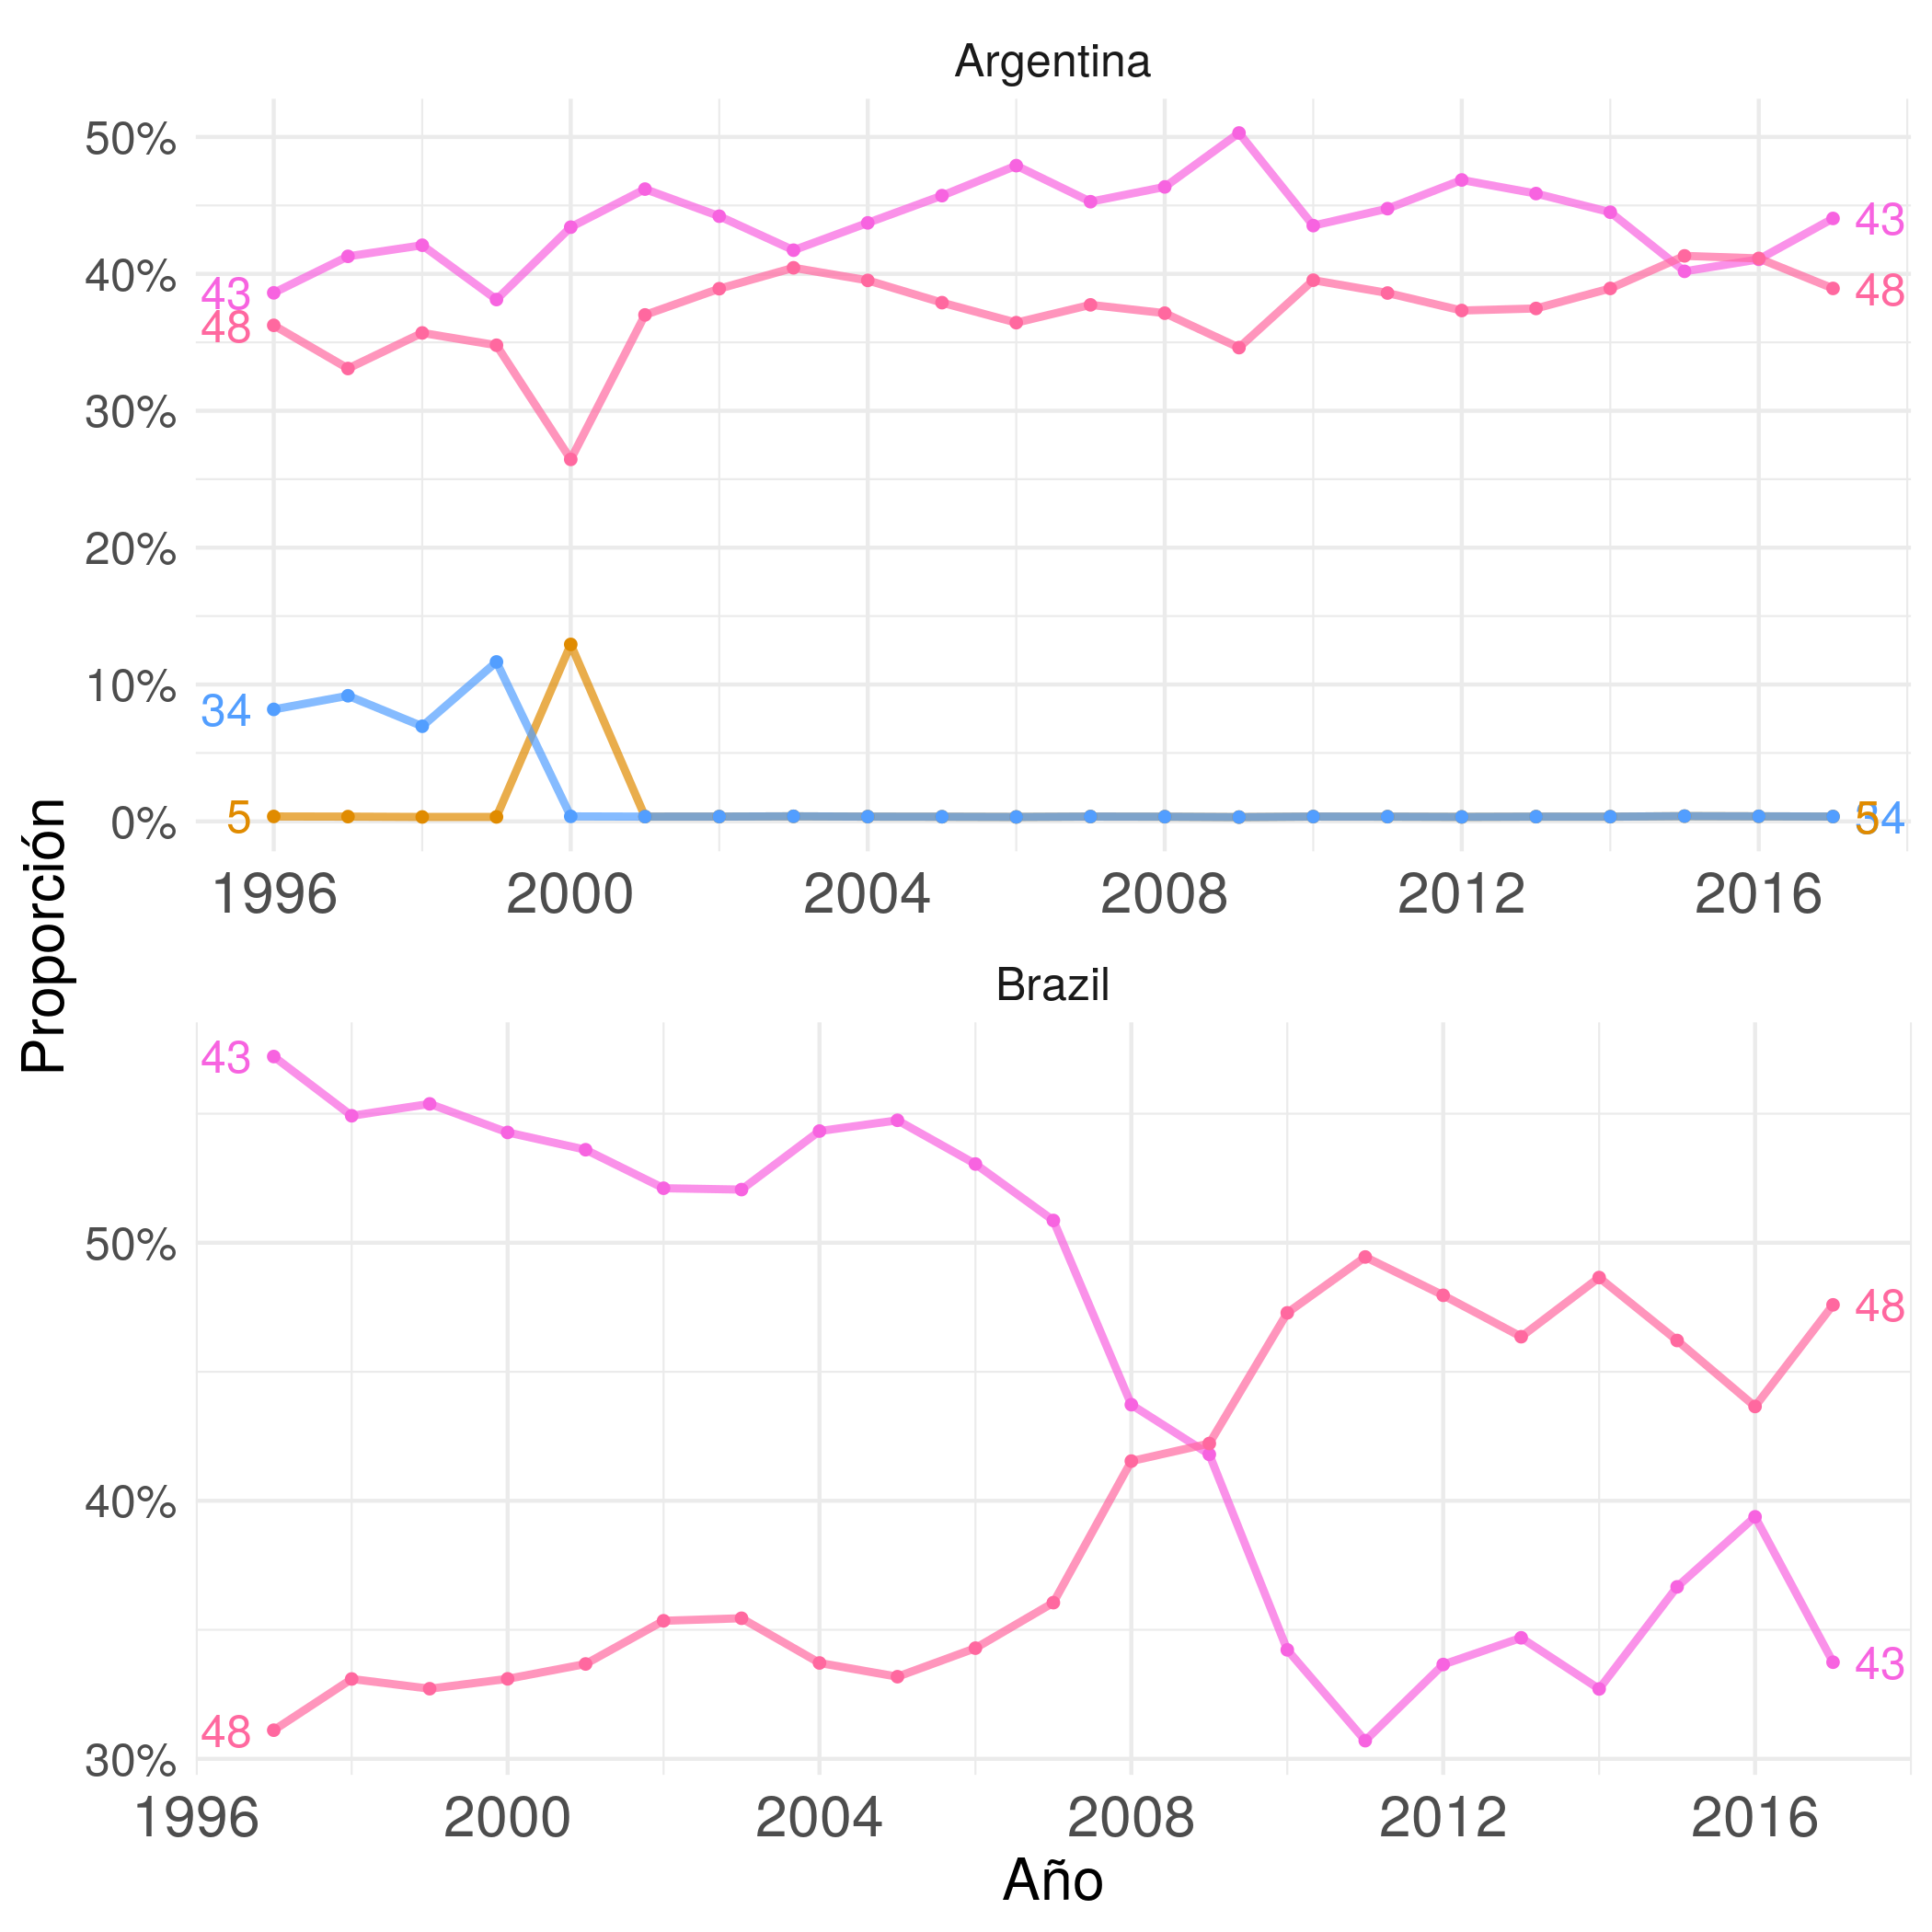
\includegraphics[width=0.7\linewidth]{images/graficoLDA_k50Arg_Bra}
	\caption{Evolución de componentes. Argentina y Brasil. K=50. Exportaciones}
	\label{fig:graficoldak50argbra}
\end{figure}

\begin{figure}
	\centering
	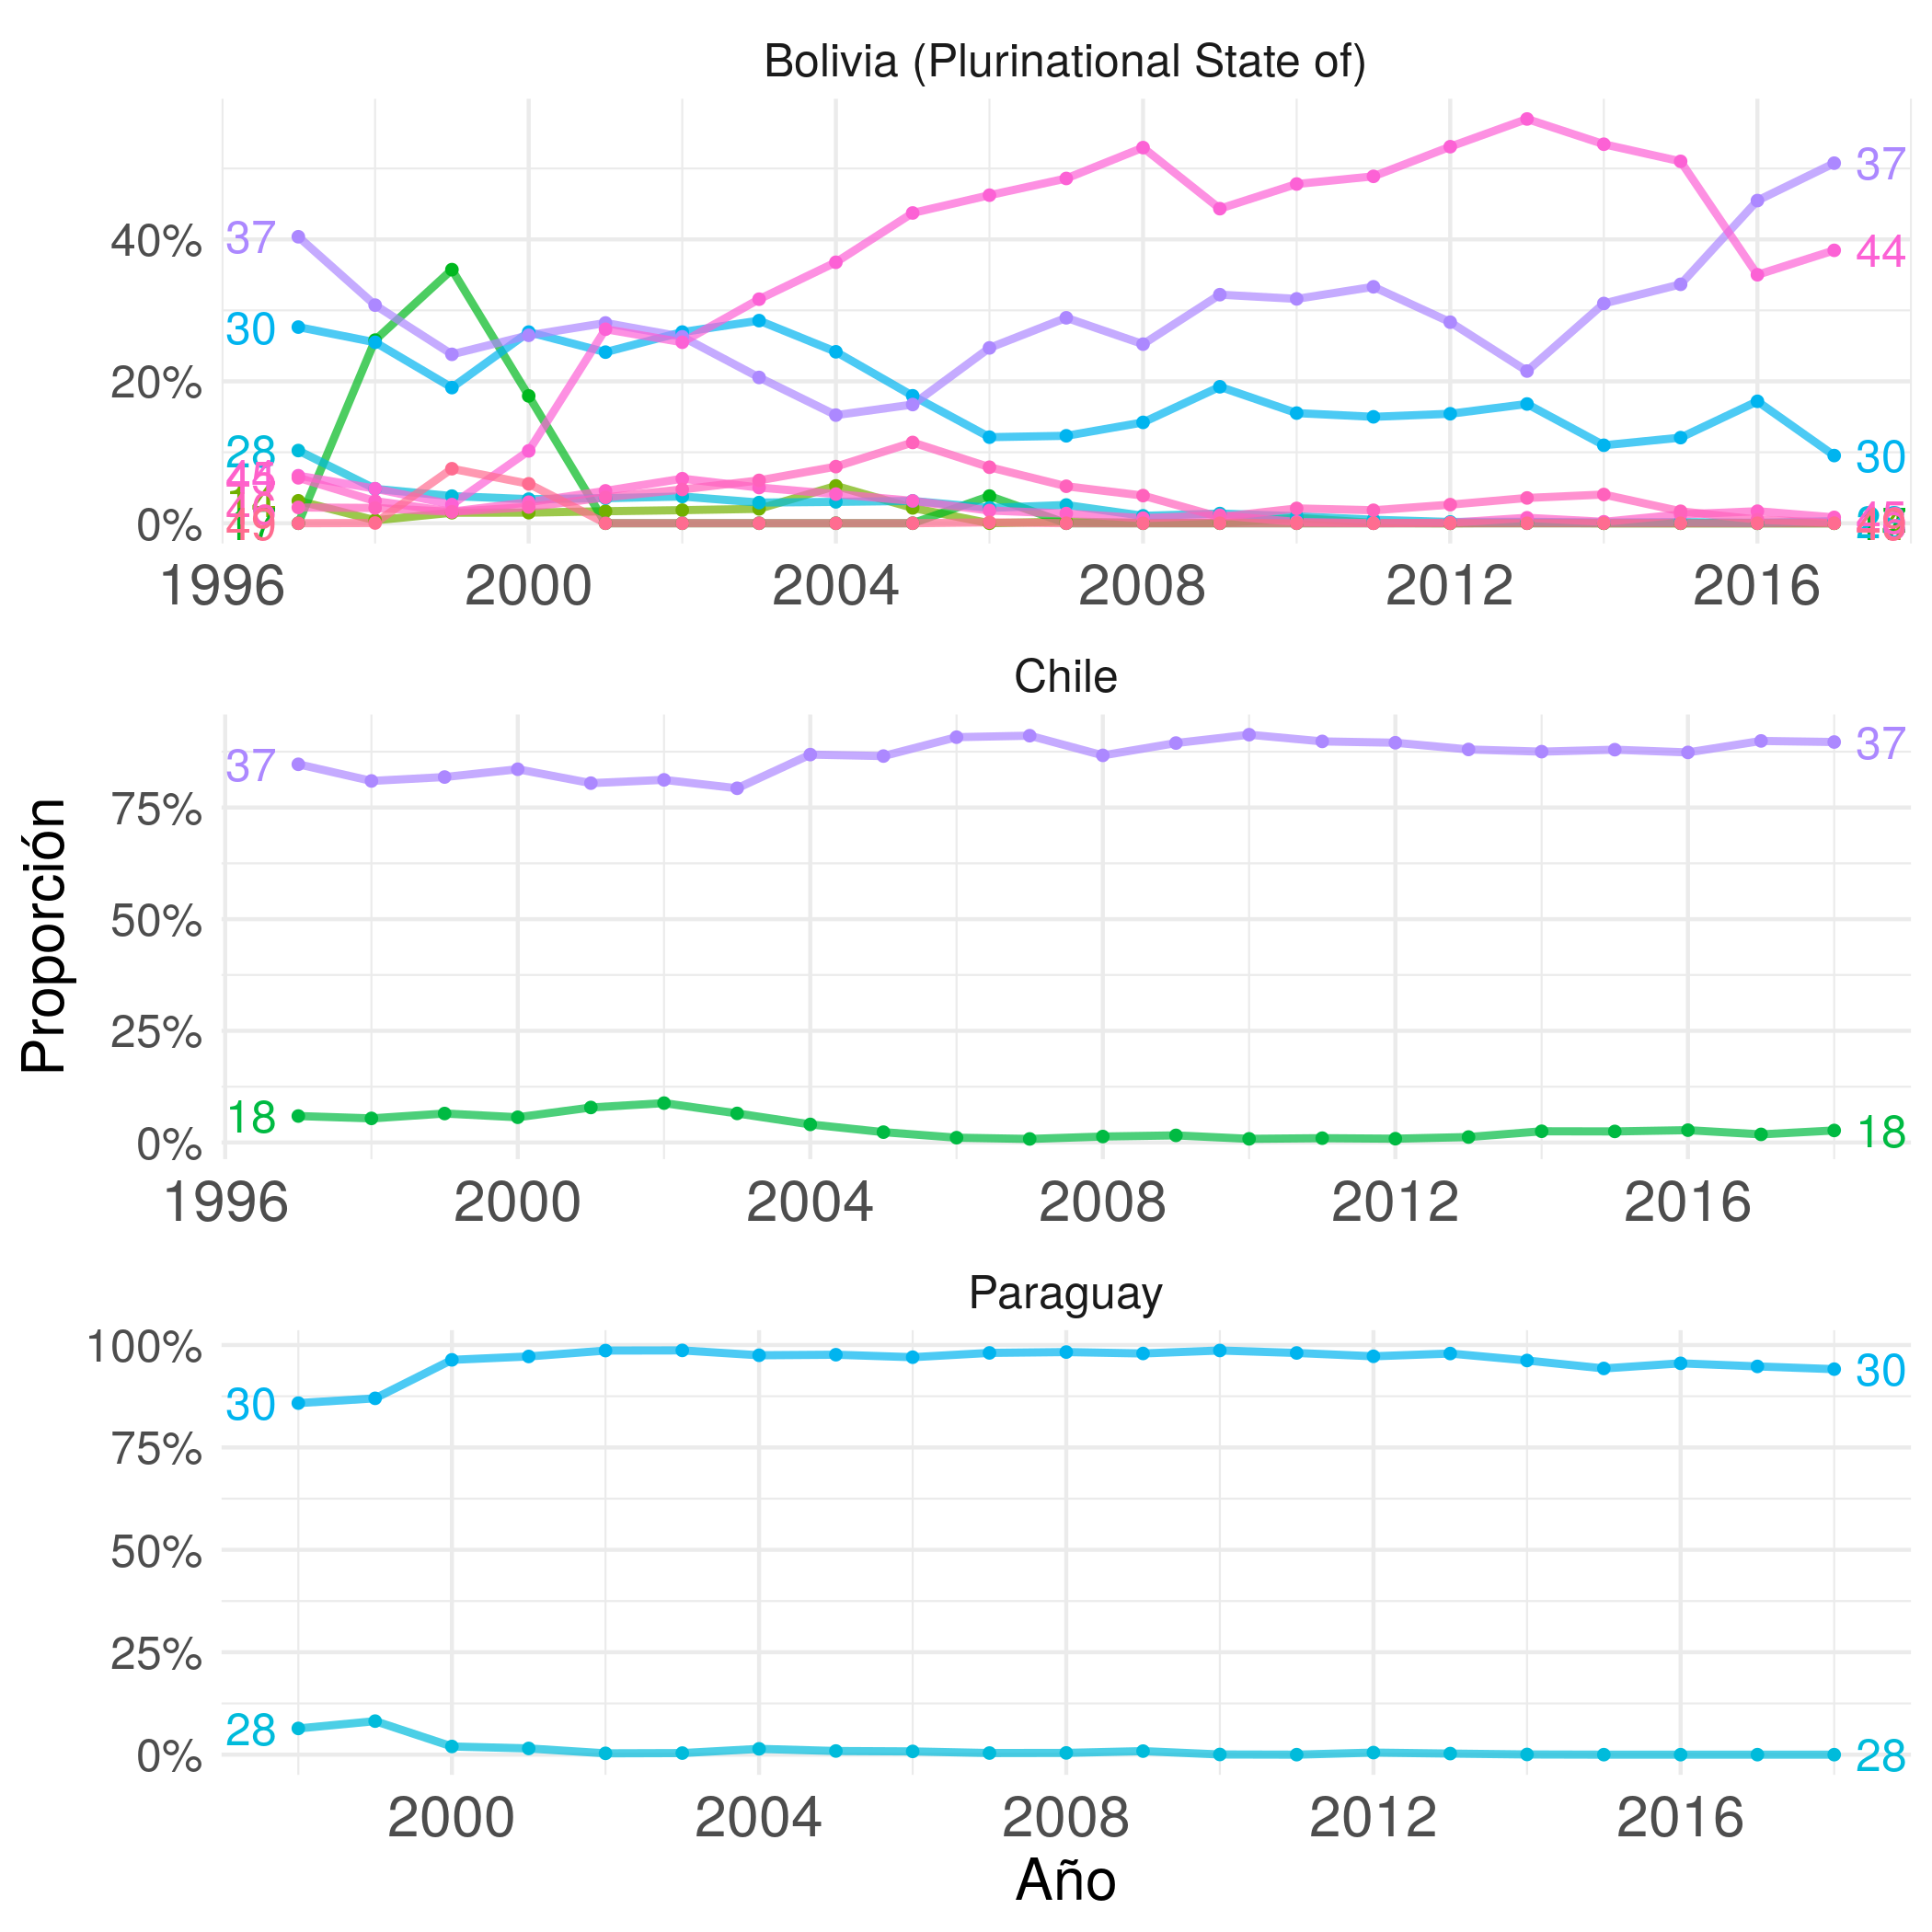
\includegraphics[width=0.7\linewidth]{images/graficoLDA_k50_bol_chi_pa}
	\caption{Evolución de componentes. Bolivia, Chile, Paraguay. K=50. Exportaciones}
	\label{fig:graficoldak50bolchipa}
\end{figure}

\begin{figure}
	\centering
	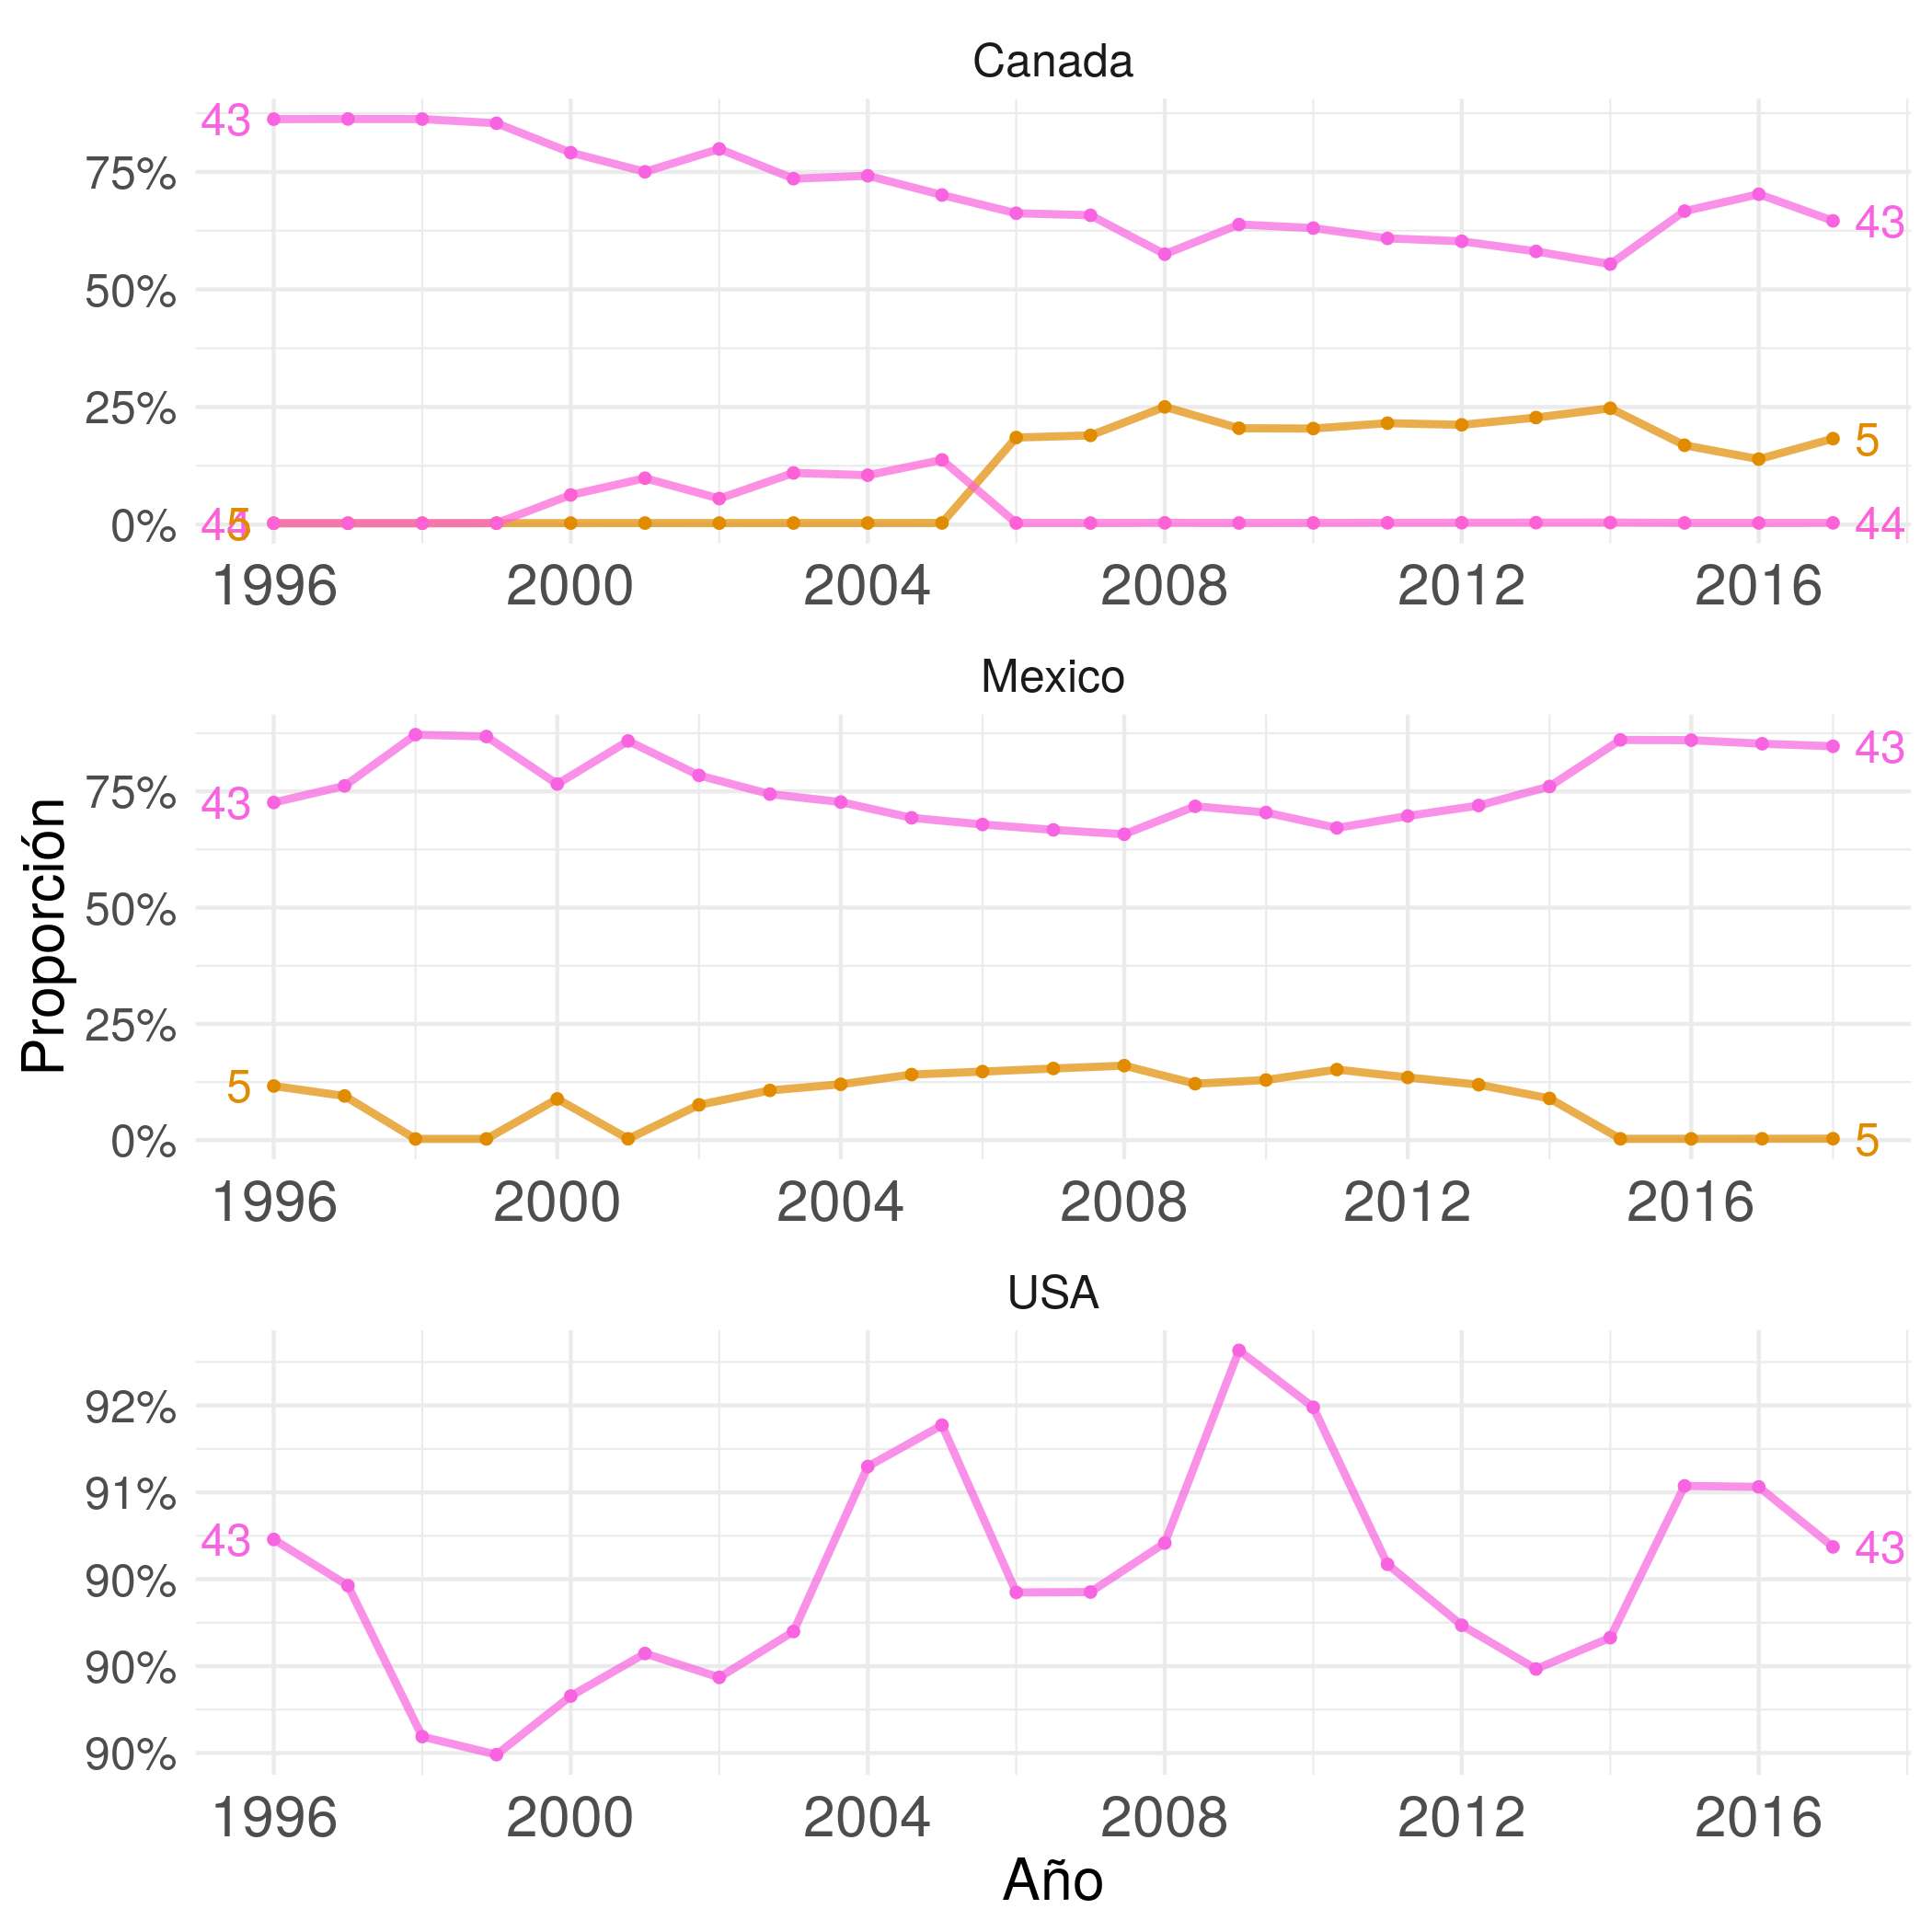
\includegraphics[width=0.7\linewidth]{images/graficoLDA_k50_us_mex_can}
	\caption{Evolución de componentes. Estados Unidos, Canadá y Mexico. Exportaciones}
	\label{fig:graficoldak50usmexcan}
\end{figure}


\begin{figure}
	\centering
	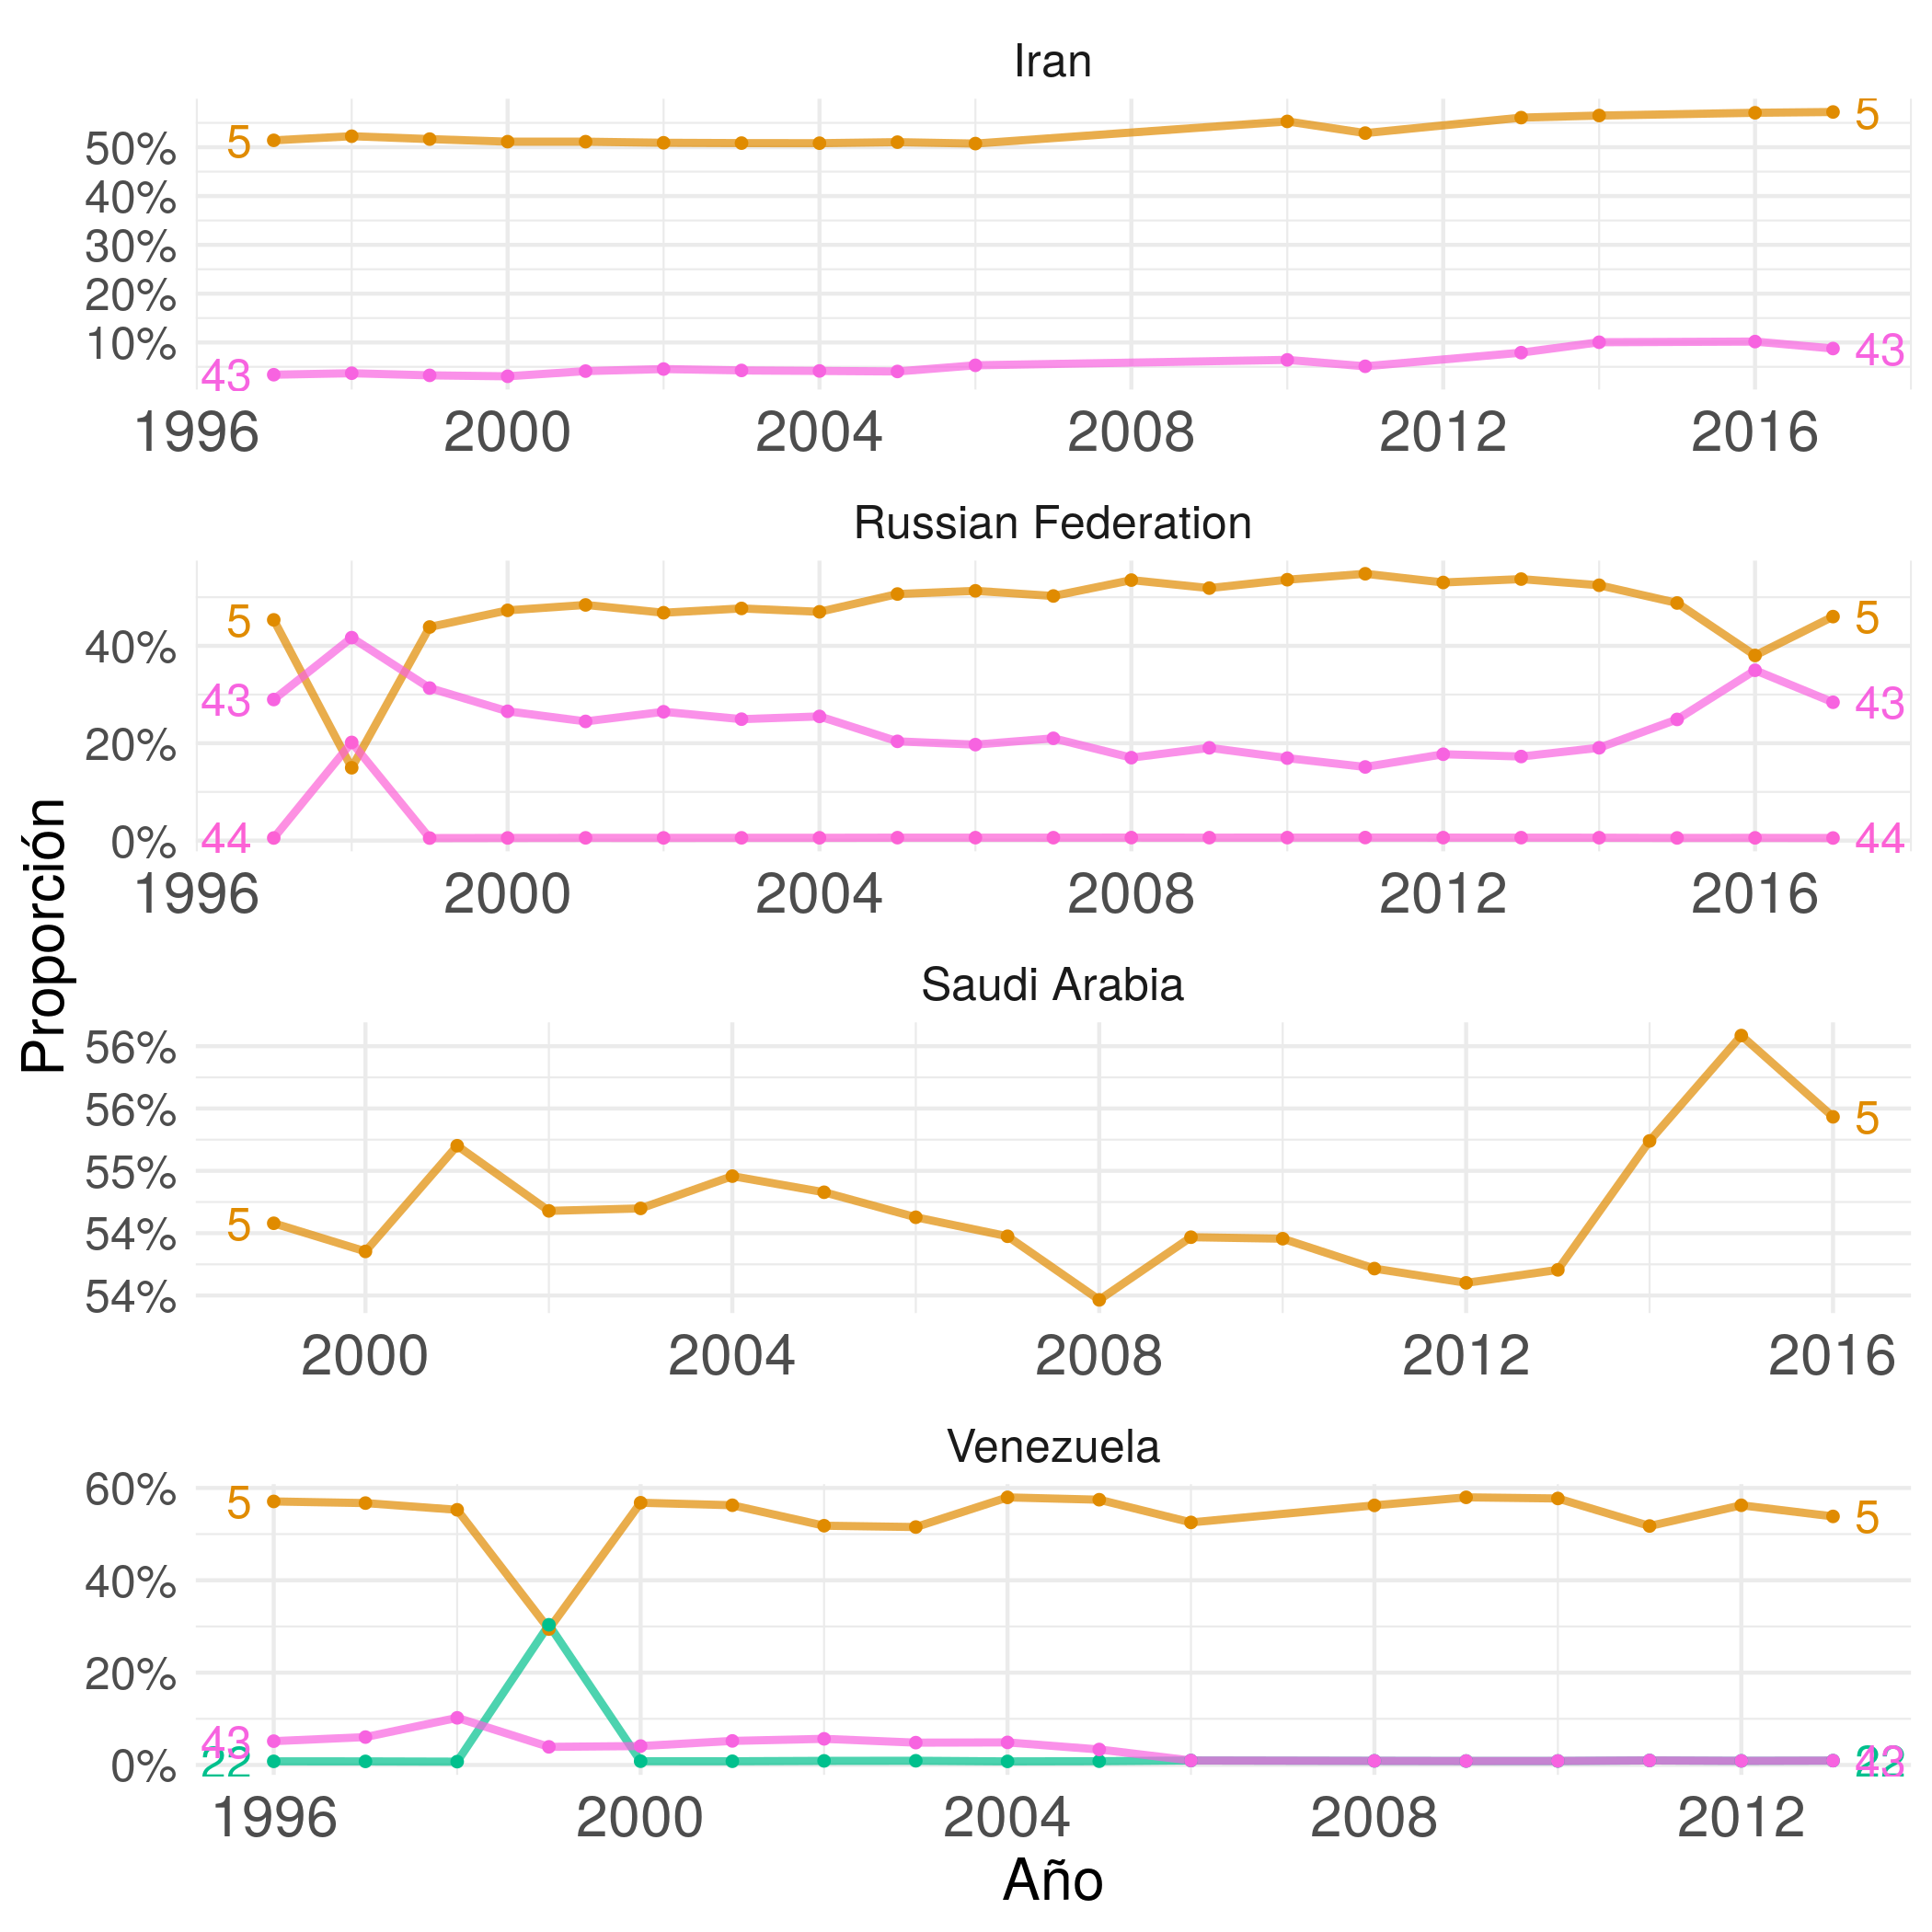
\includegraphics[width=0.7\linewidth]{images/graficoLDA_k50_ir_rus_sa_ven}
	\caption{Evolución de componentes. Países petroleros. Exportaciones.}
	\label{fig:graficoldak50irrussaven}
\end{figure}


\begin{figure}
	\centering
	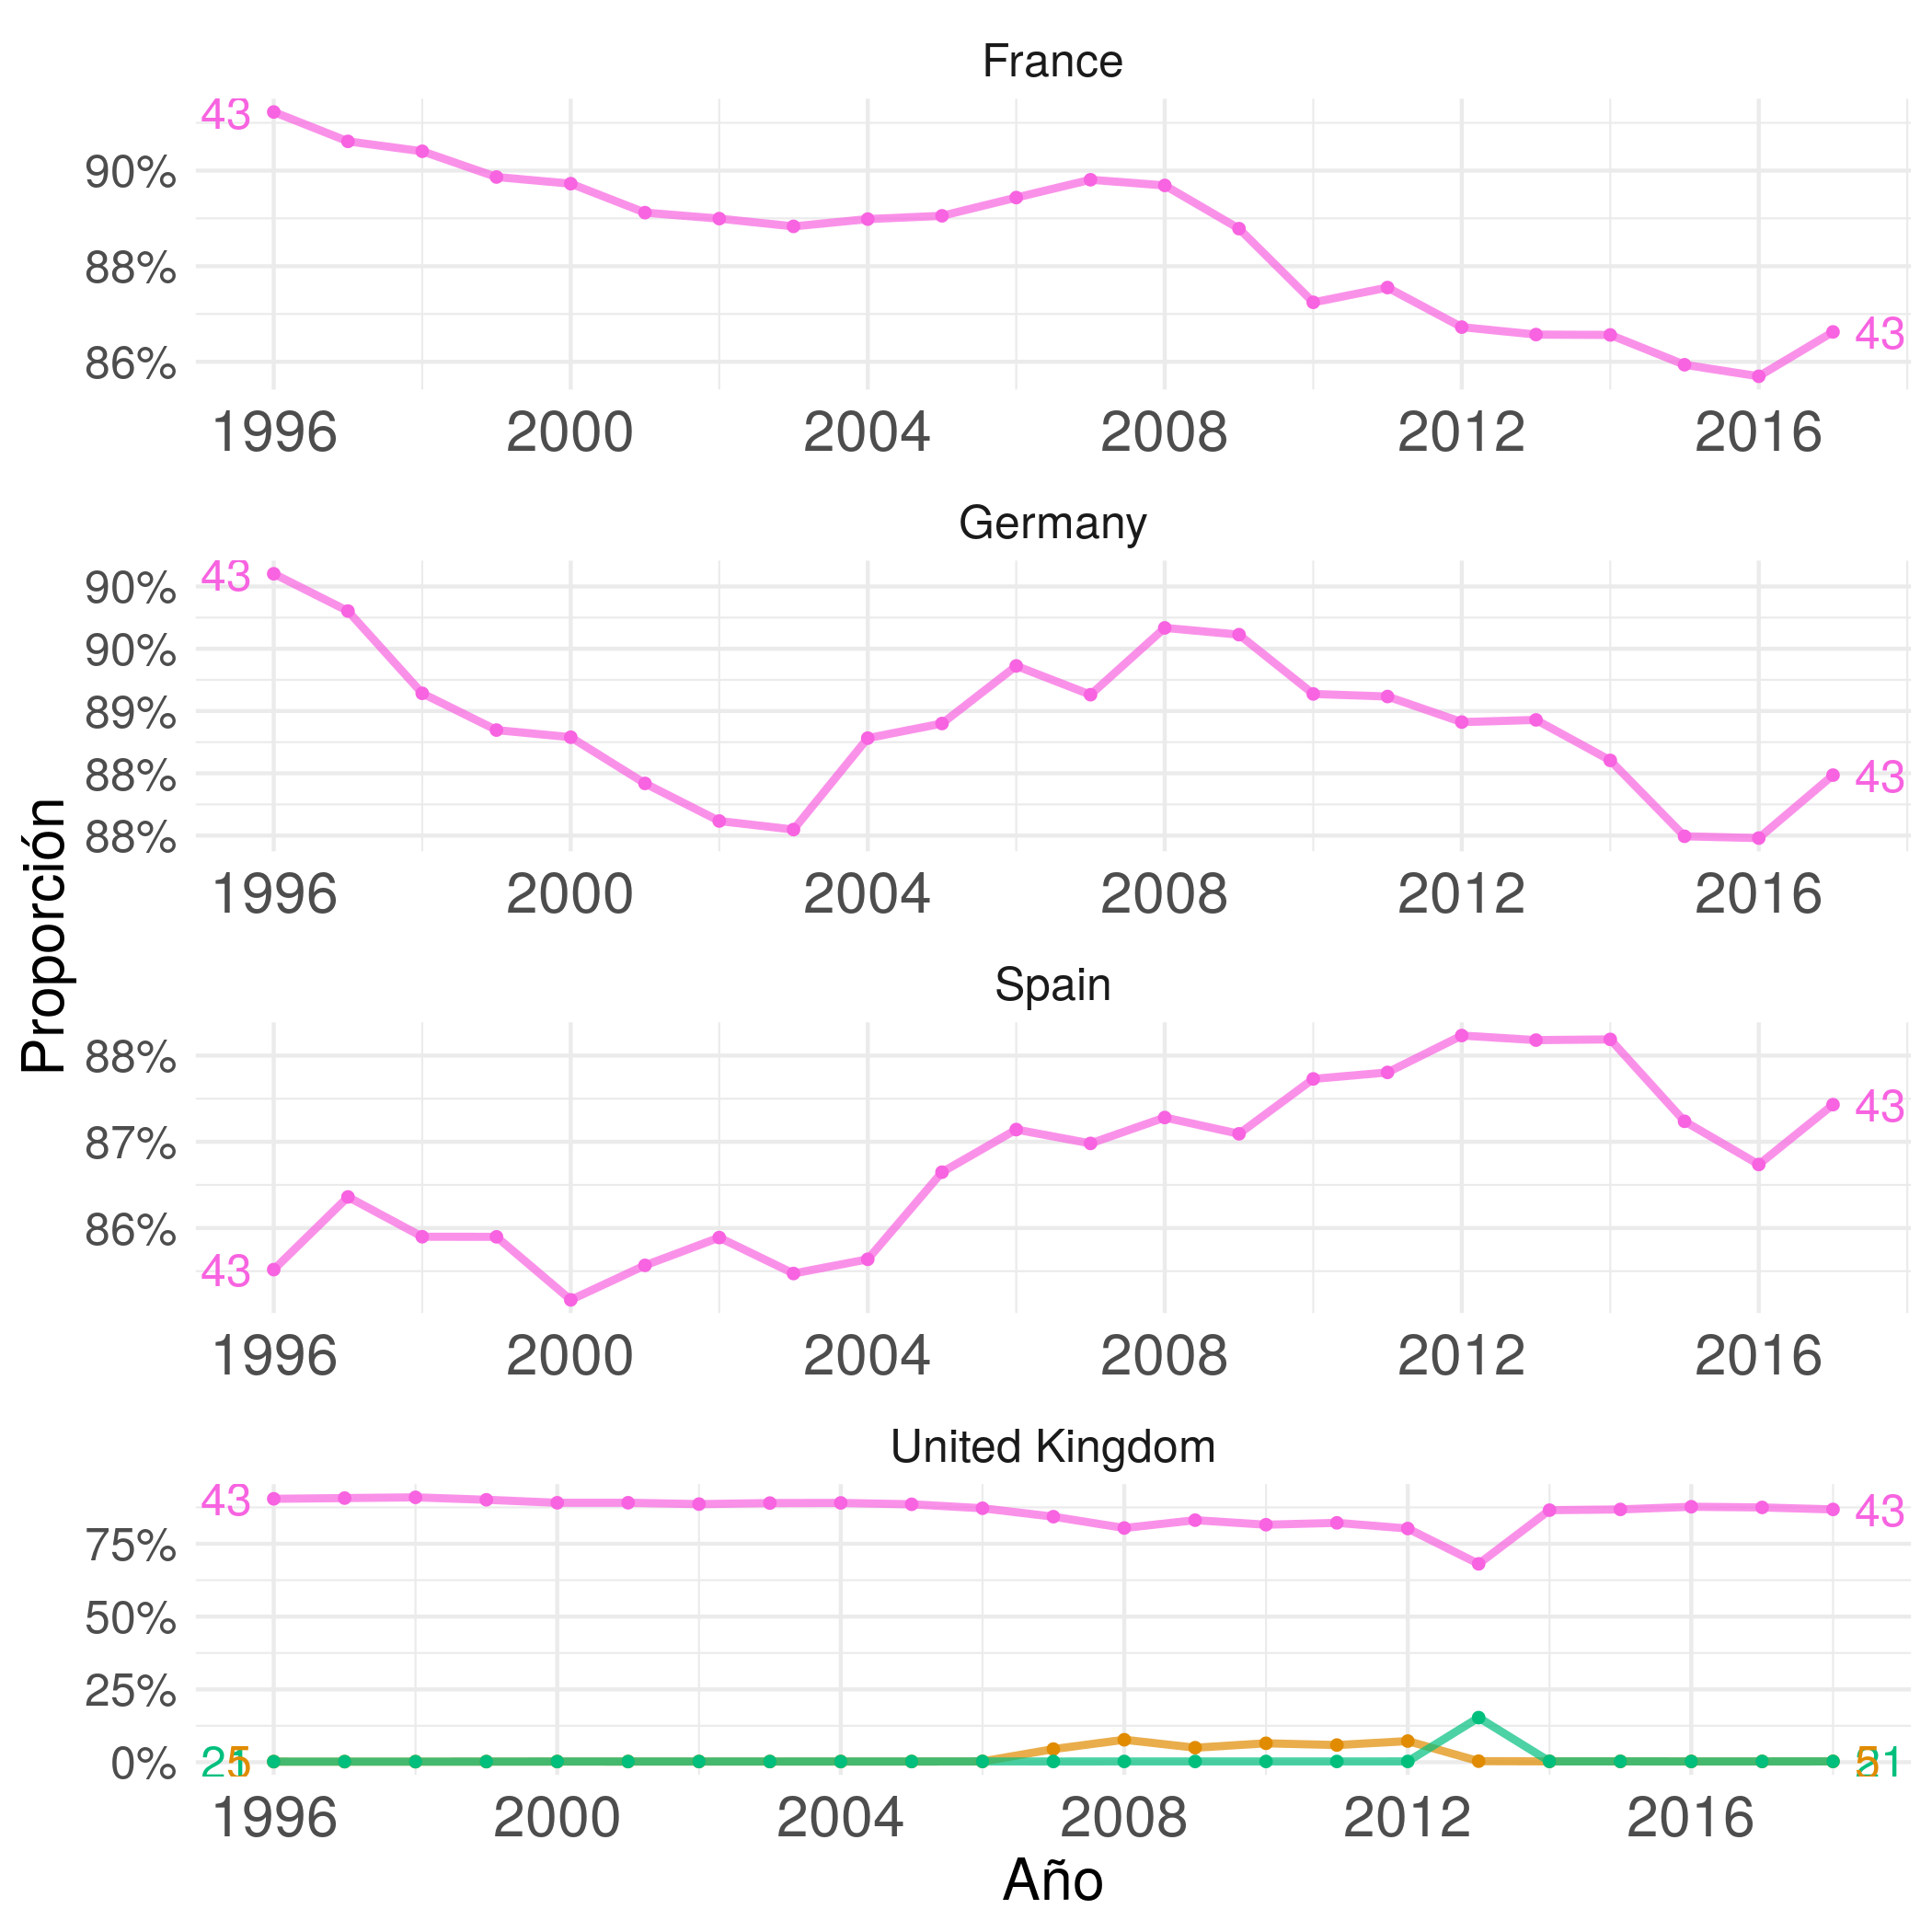
\includegraphics[width=0.7\linewidth]{images/graficoLDA_k50_uk_fr_esp_ger}
	\caption{Evolución de componentes. Países europeos. Exportaciones}
	\label{fig:graficoldak50ukfrespger}
\end{figure}




\begin{figure}
	\centering
	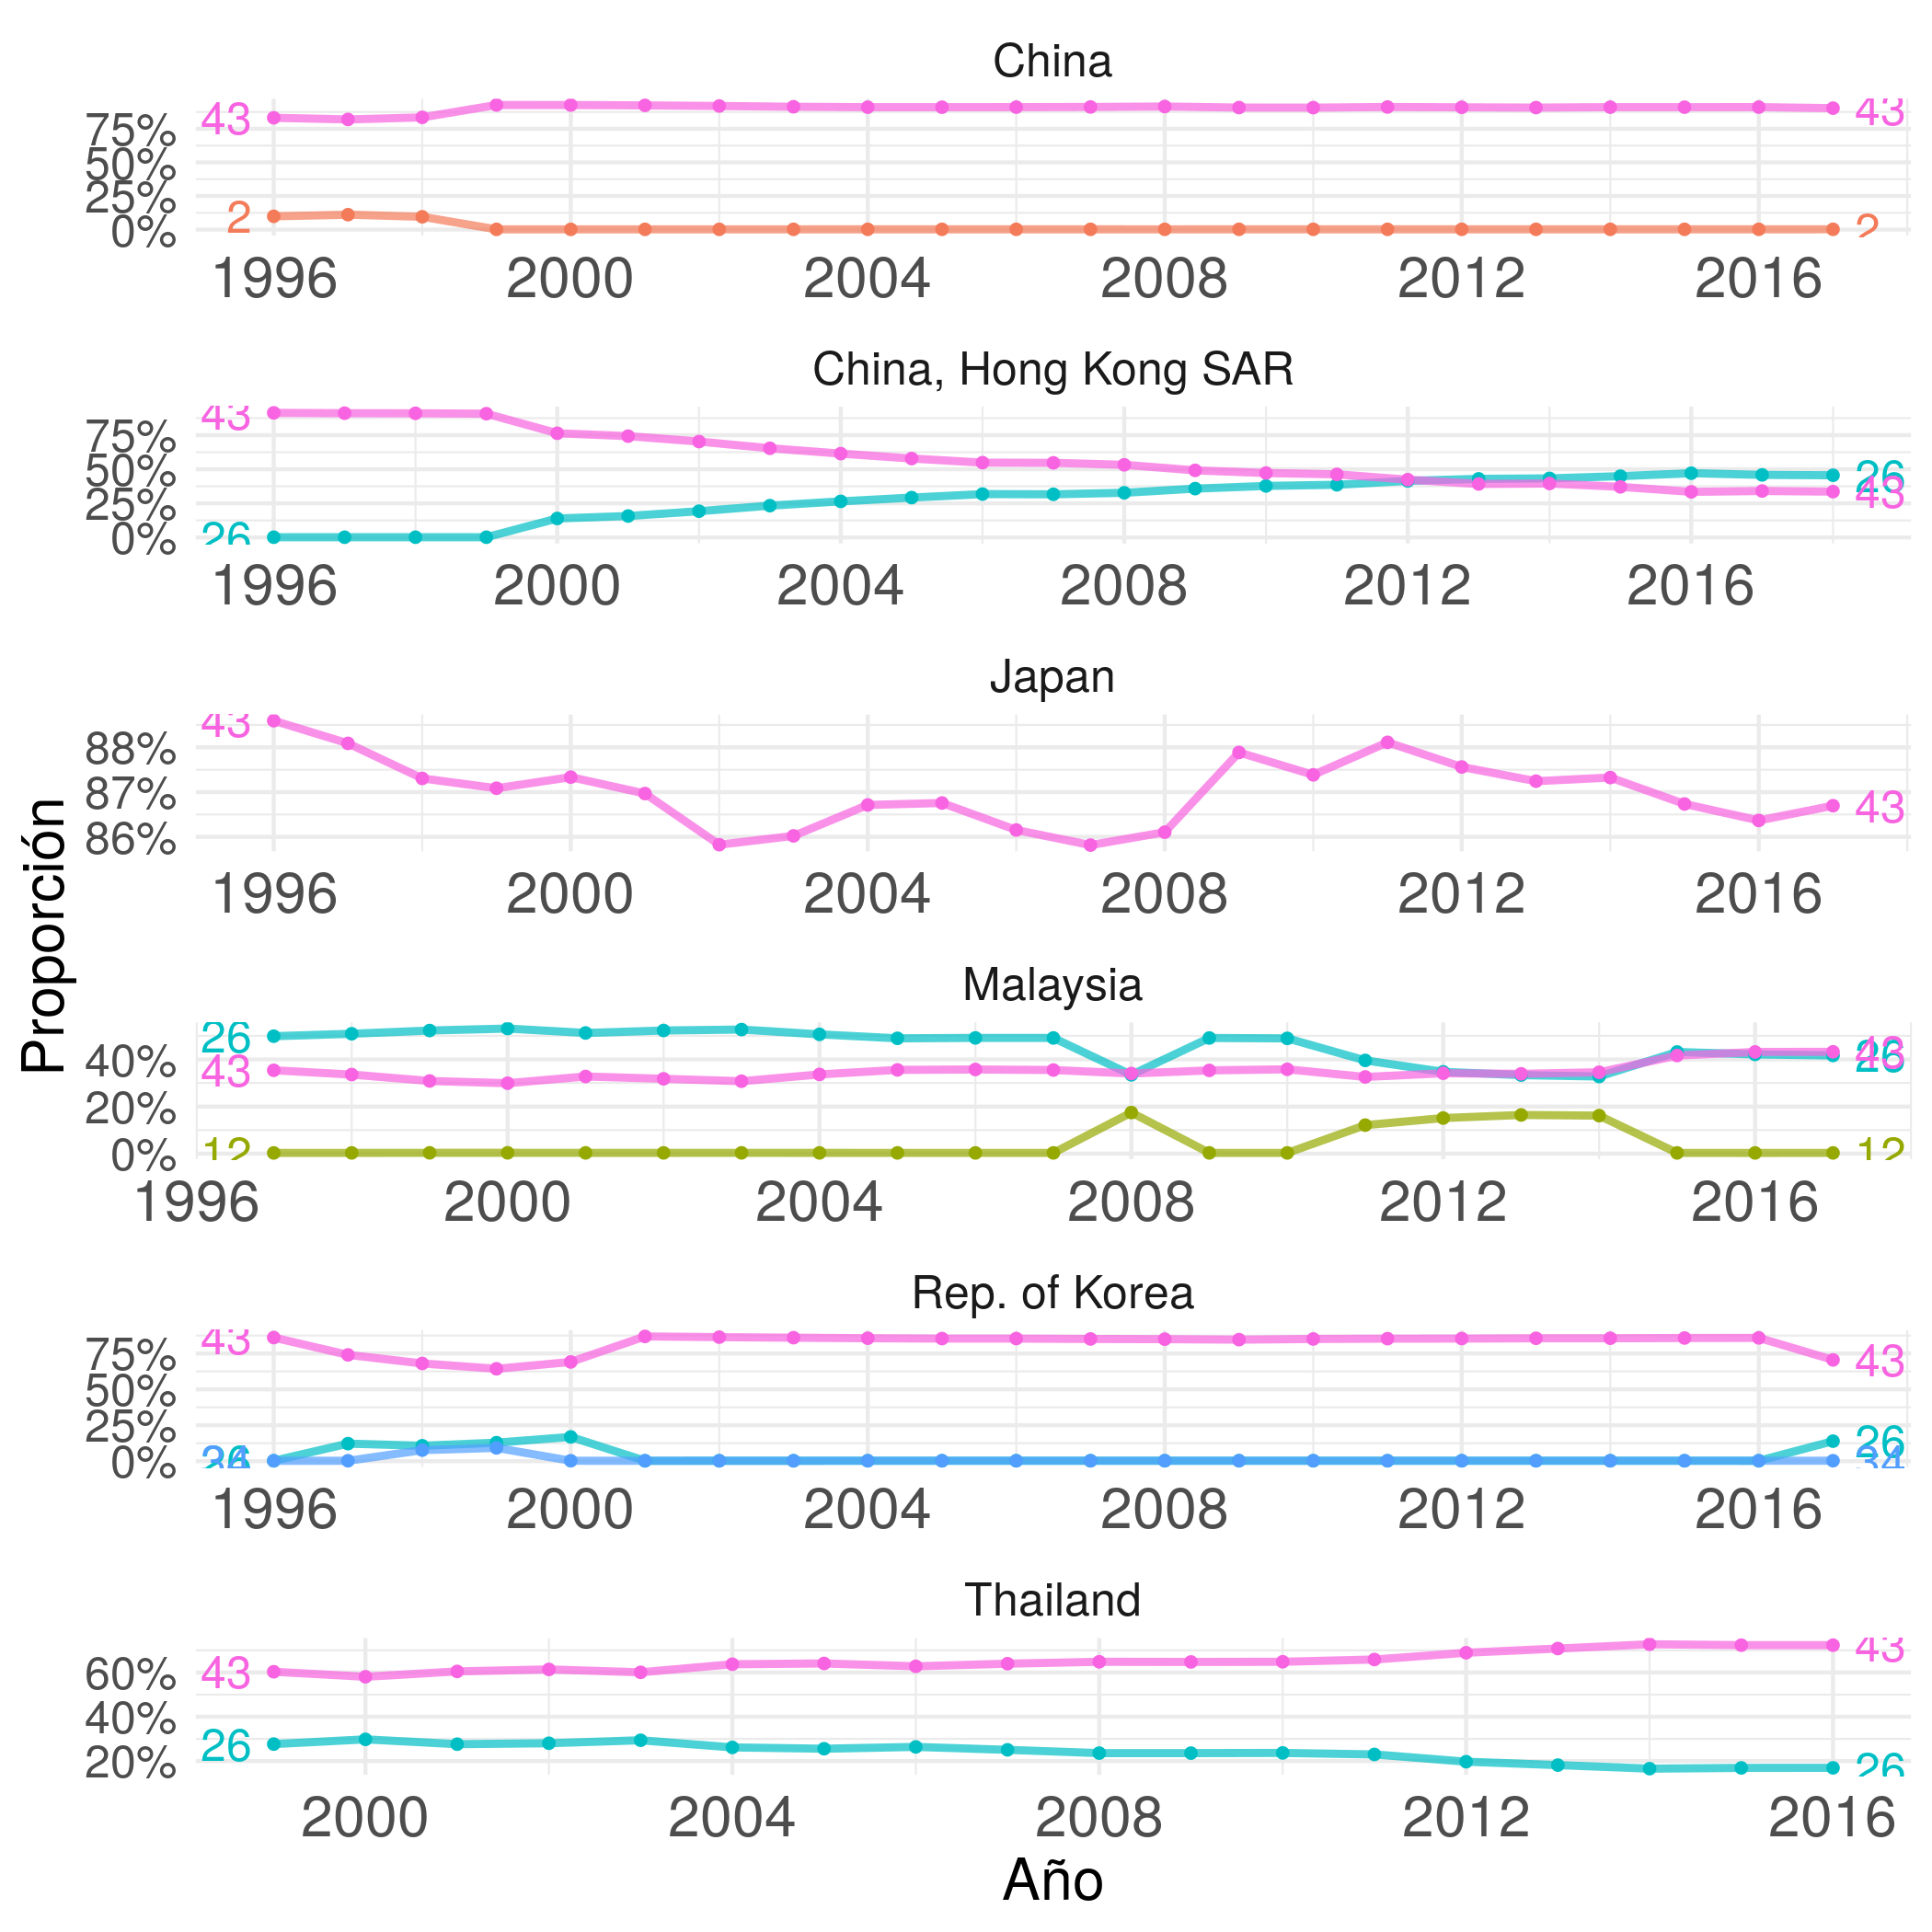
\includegraphics[width=0.8\linewidth]{images/graficoLDA_k50_asia}
	\caption{Evolución de componentes. Asia. Exportaciones}
	\label{fig:graficoldak50asia}
\end{figure}


\begin{figure}
	\centering
	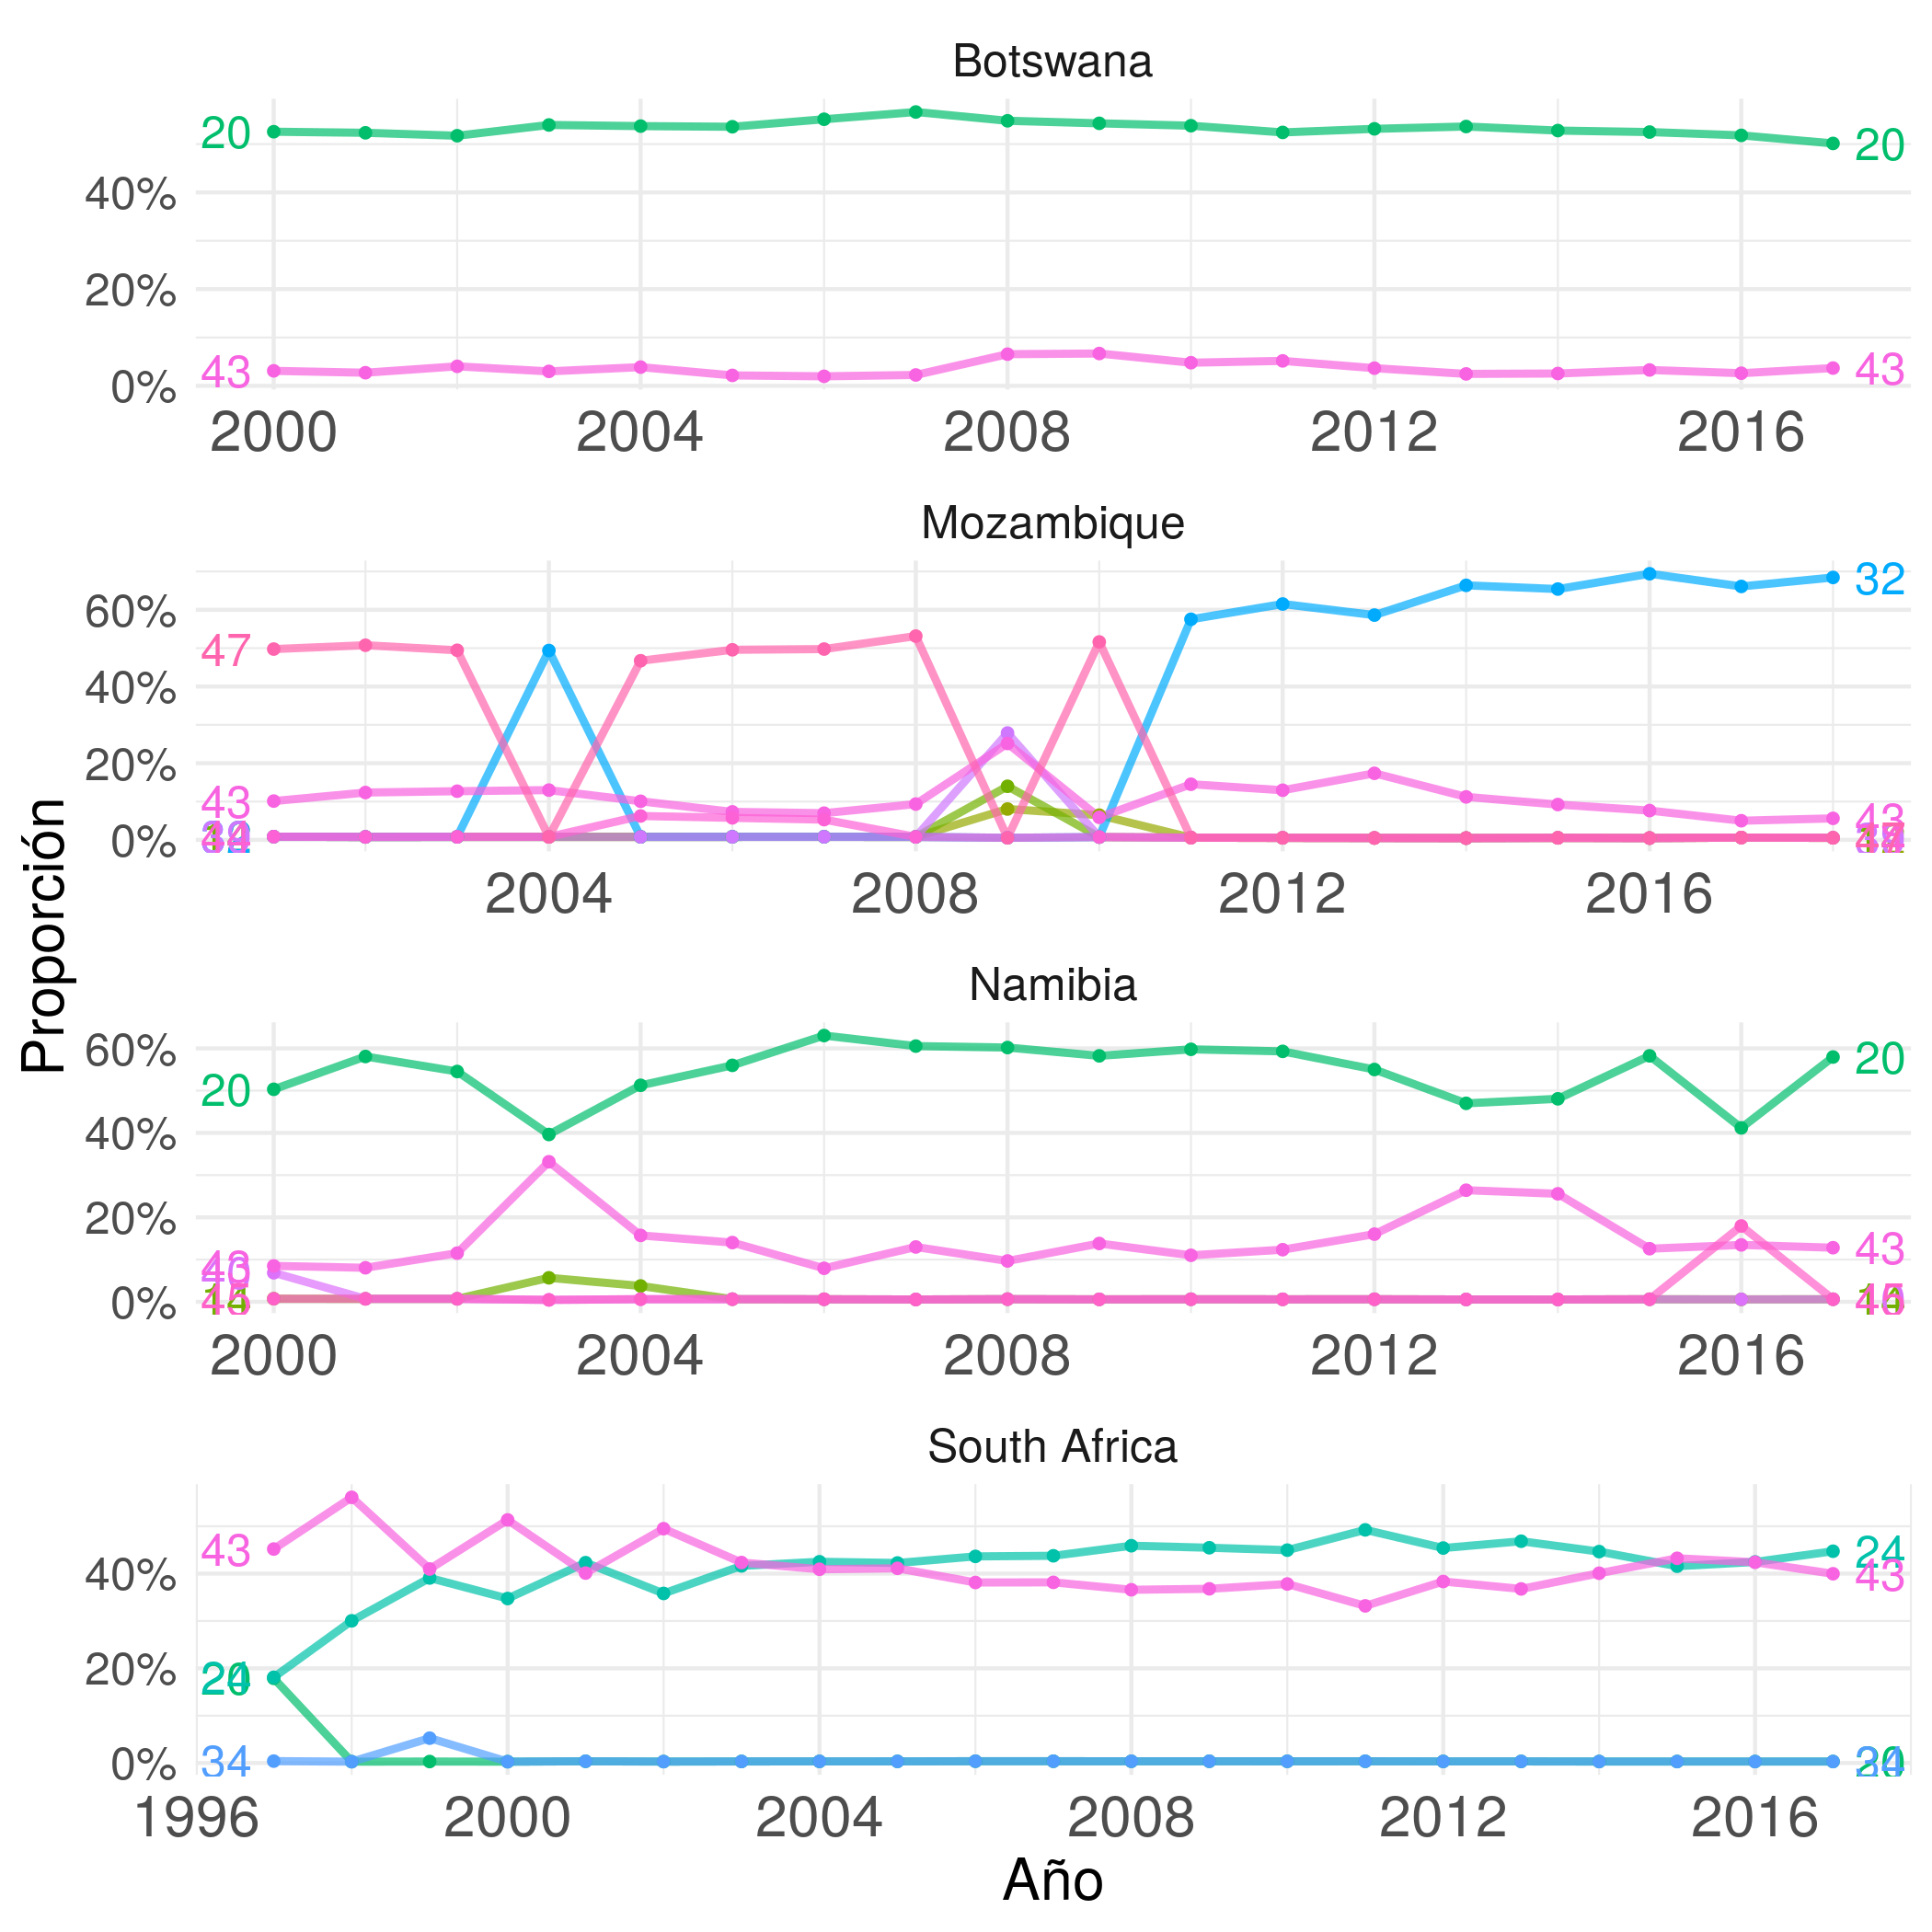
\includegraphics[width=0.7\linewidth]{images/graficoLDA_k50_africa_austral}
	\caption{Evolución de componentes. África Austral. Exportaciones}
	\label{fig:graficoldak50africaaustral}
\end{figure}

\begin{figure}
	\centering
	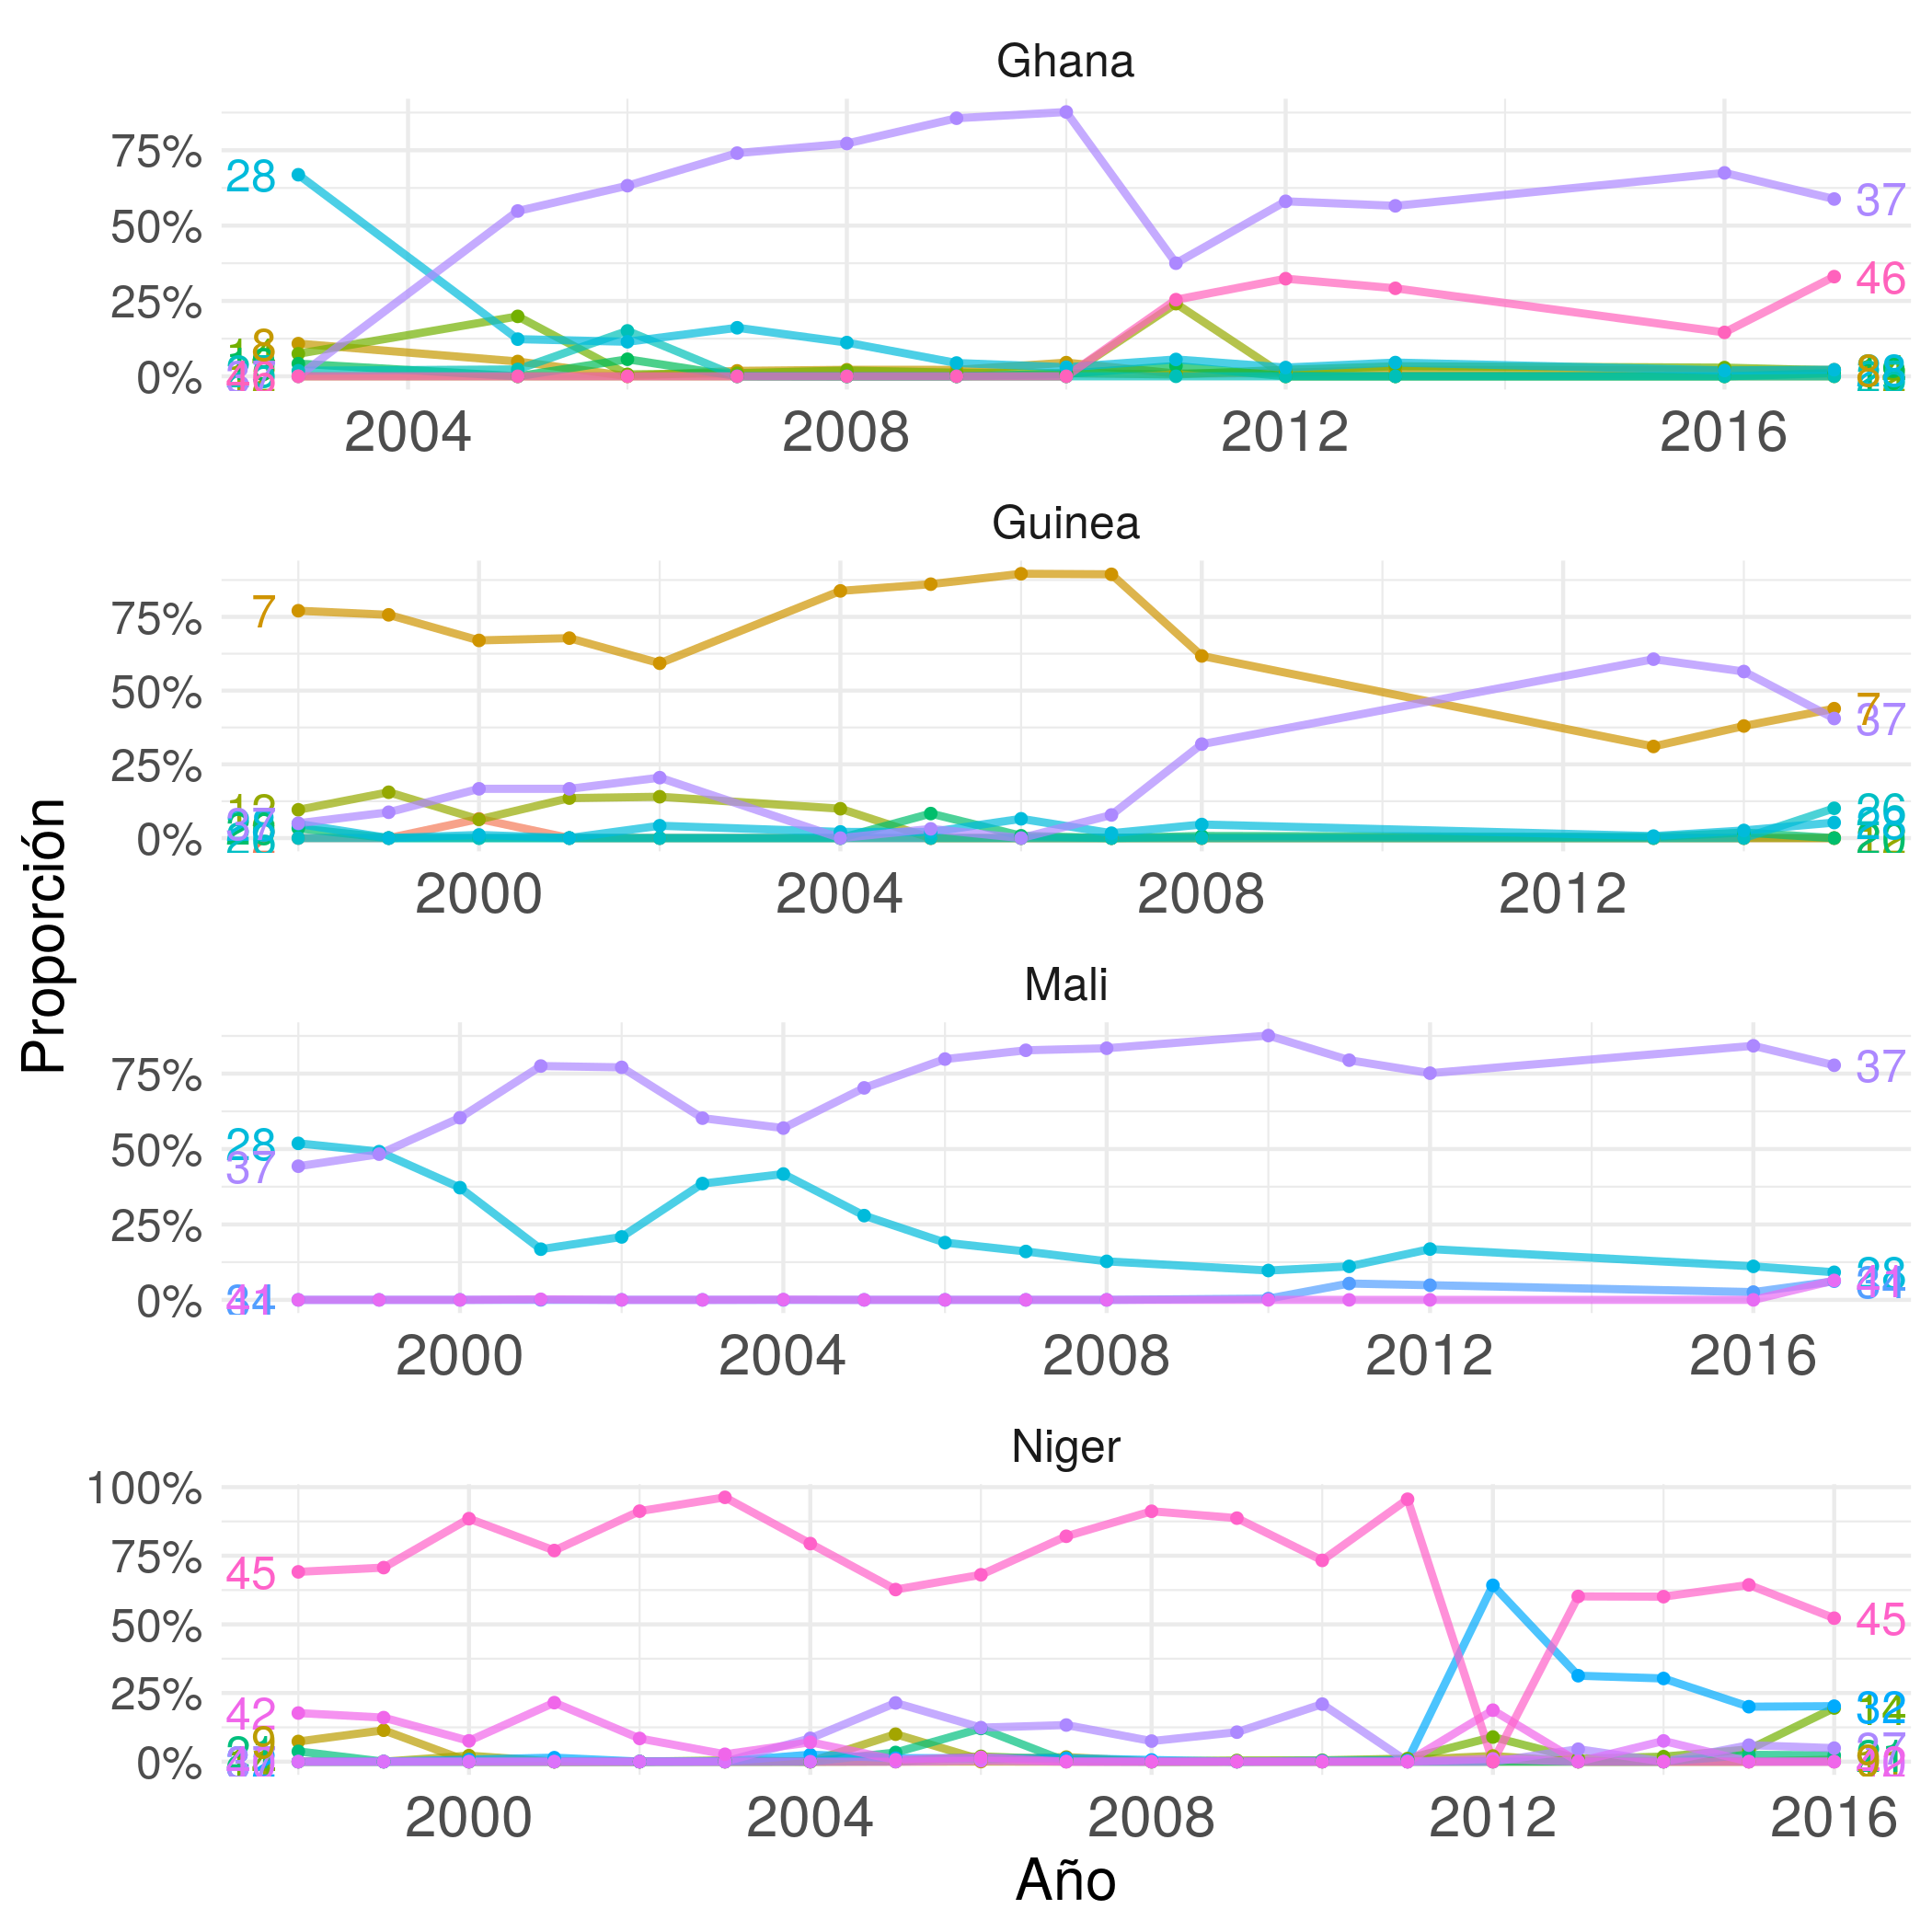
\includegraphics[width=0.7\linewidth]{images/graficoLDA_k50_africa_noroccidental}
	\caption{Evolución de componentes. África Noroccidental}
	\label{fig:graficoldak50africanoroccidental}
\end{figure}

%\begin{figure}
%	\centering
%	\subfigure[Argentina y Brasil]{\label{fig:serie_componentes_1}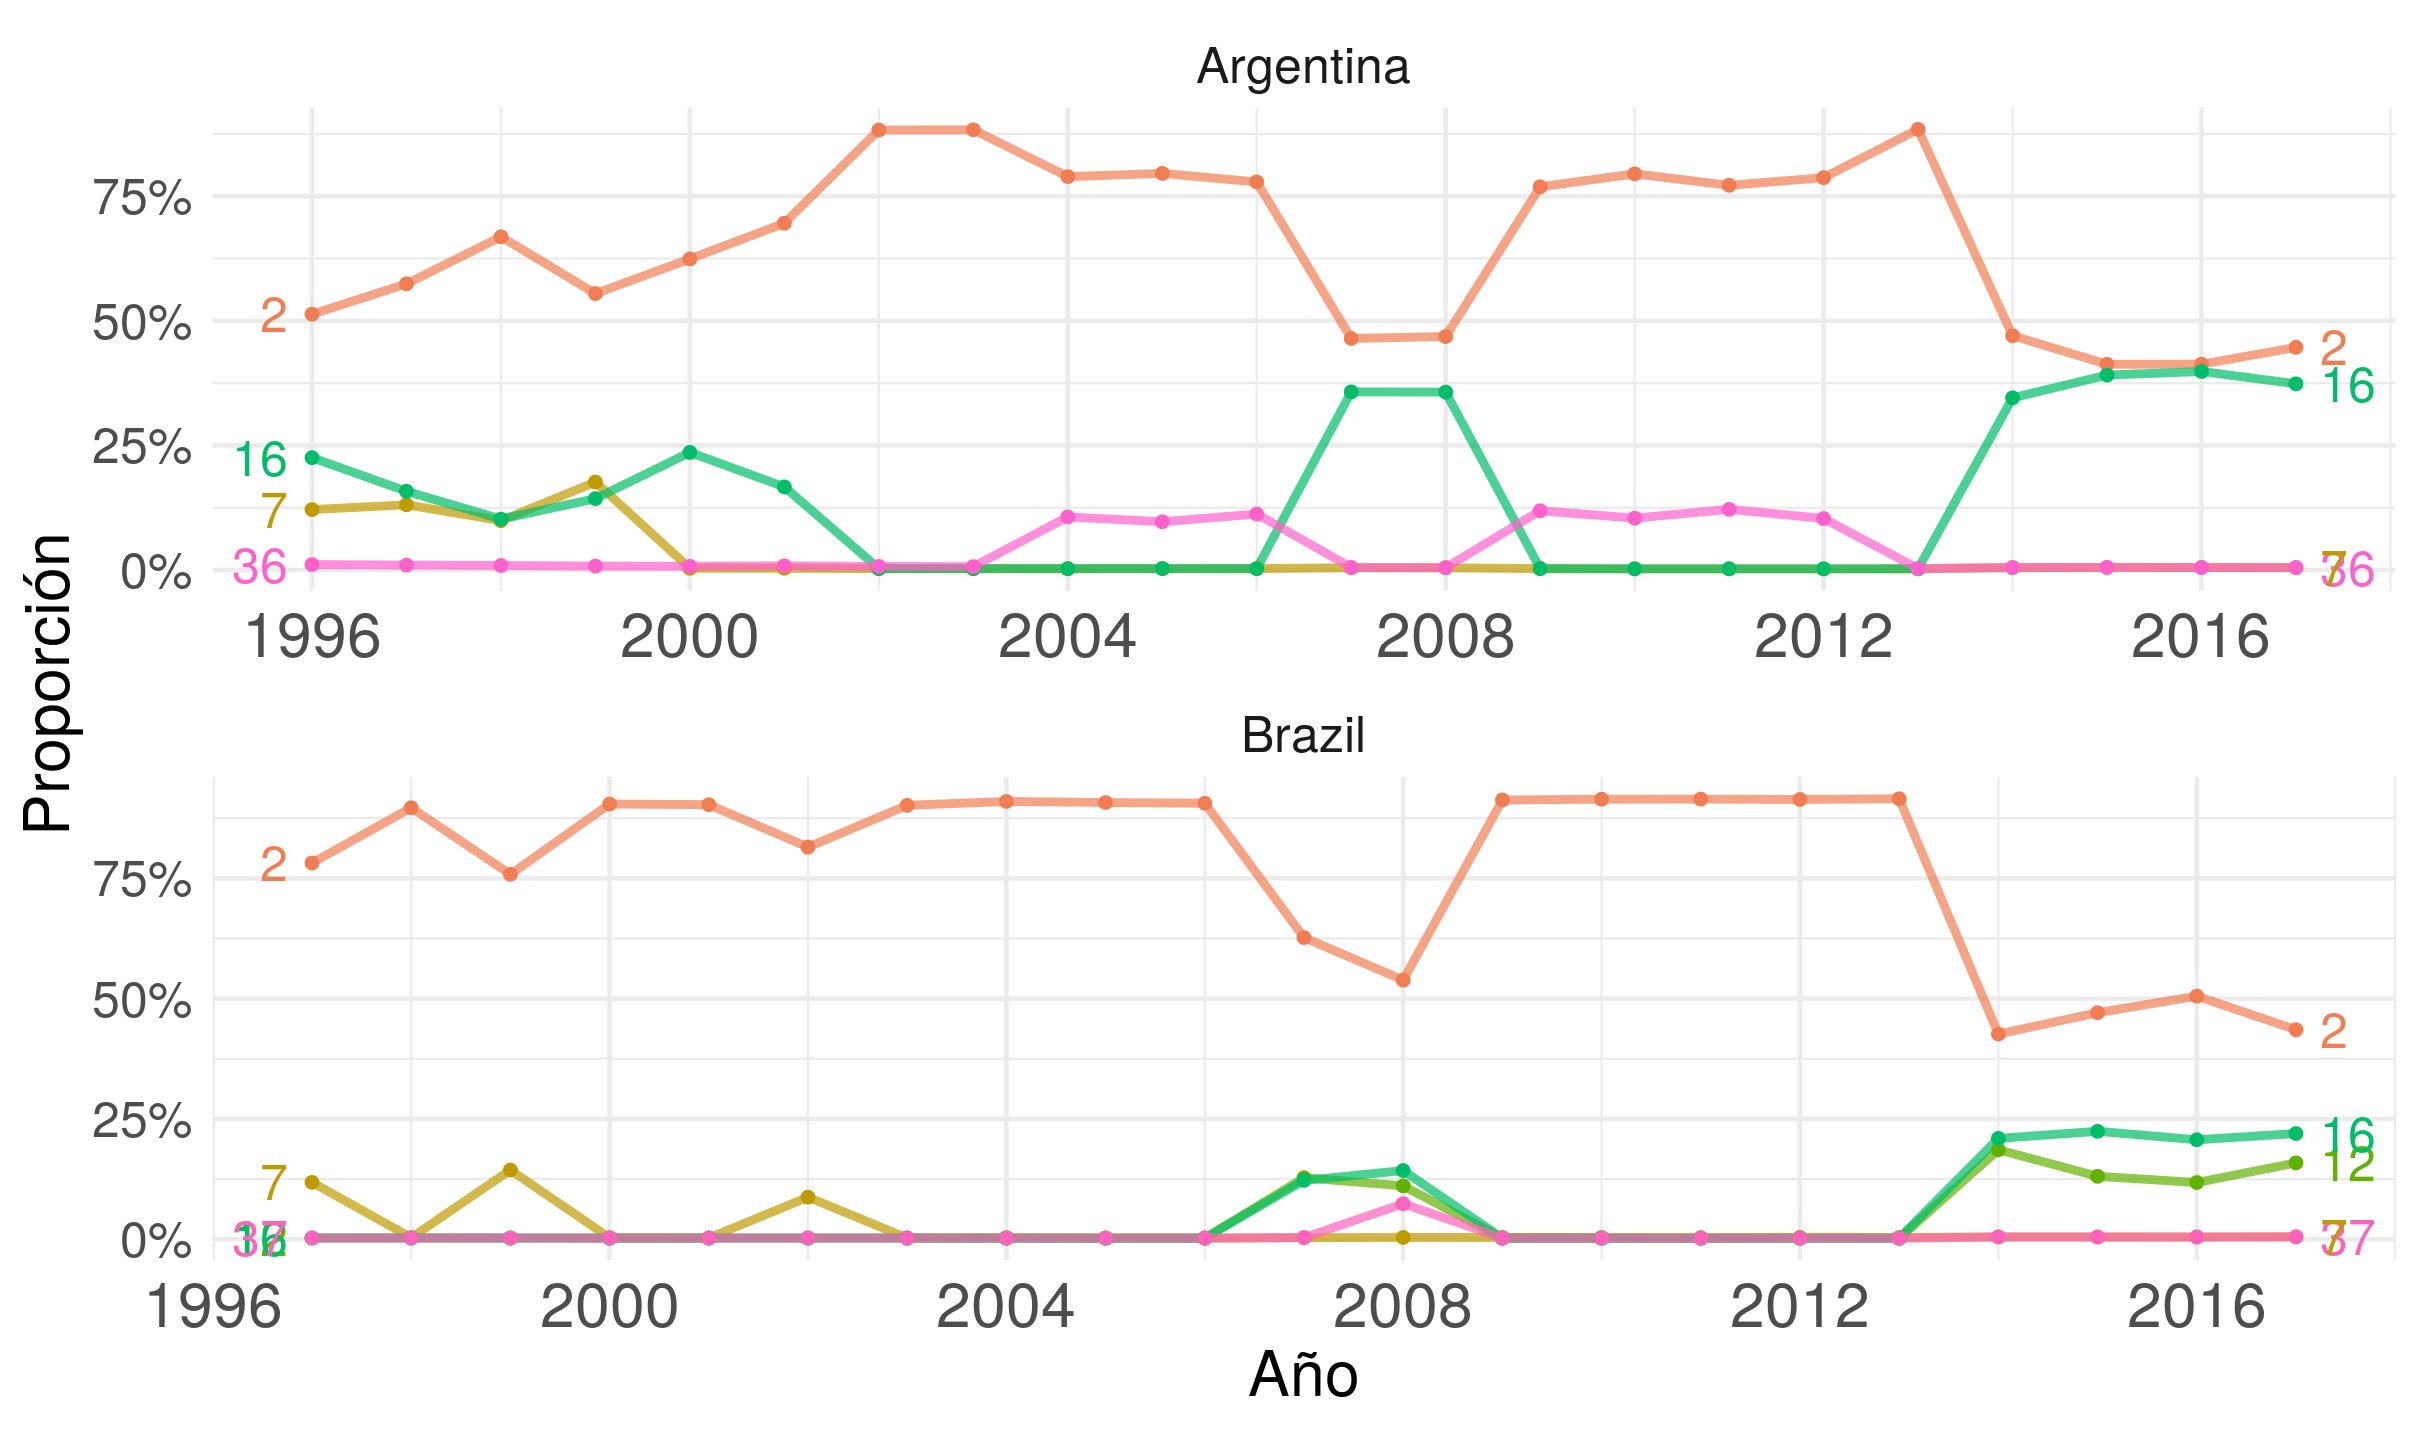
\includegraphics[width=\linewidth]{graficoLDA_k40_arg_bra}}
%	\subfigure[Bolivia, Chile y Paraguay]{\label{fig:serie_componentes_2}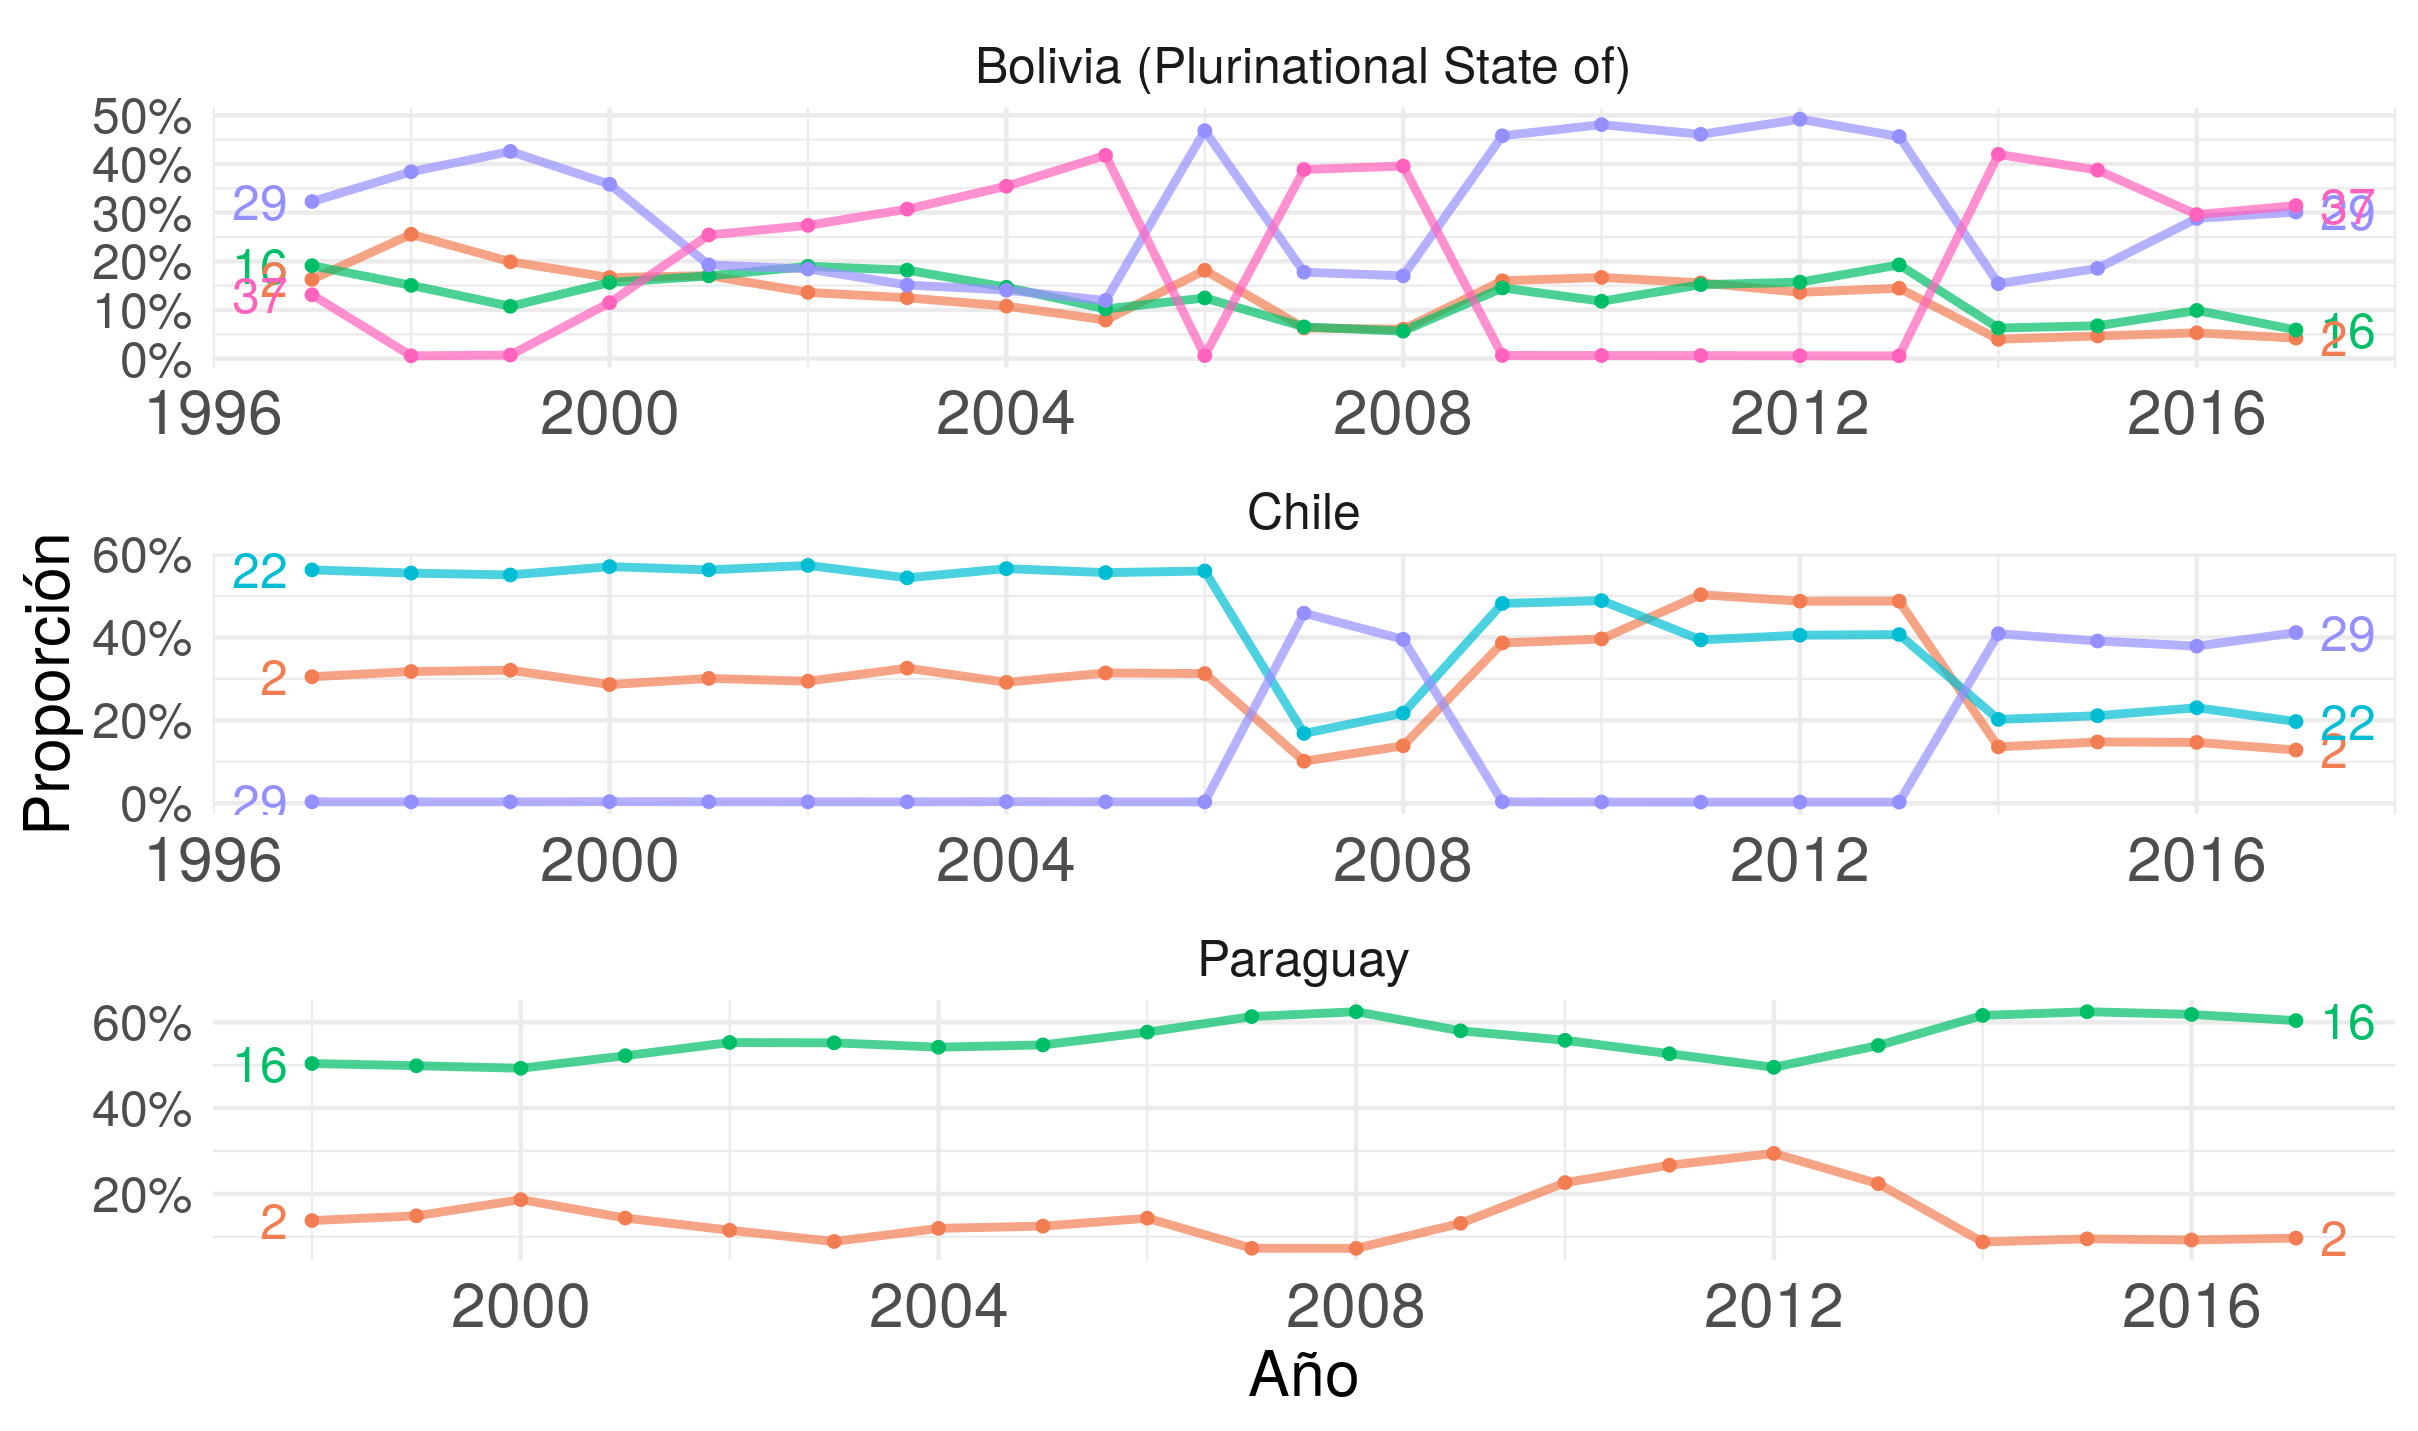
\includegraphics[width=\linewidth]{graficoLDA_k40_bol_chi_pa}}
%	\caption{Evolución componentes en Sudamérica. Exportaciones. 1997-2017}
%	\label{fig:serie_componentes}
%\end{figure} 

\subsection{Grafo Bipartito}

\subsubsection{Proyección a nivel países}

Como se mencionó en la metodología, se realizó una proyección del grafo bipartito para reconstruir un grafo simple ponderado de la similitud de la estructura productiva de los países. sobre la base de esto, se realizó un análisis de comunidades. En la figura \ref{fig:mapas_proyeccion} se puede observar las comunidades detectadas para el año 2016. En \ref{fig:mapas_proyeccion_1} se puede observar las comunidades obtenidas mediante la técnica de \textit{Louvain}. Con este método se encuentras tres comunidades. La primer comunidad contiene a China, India, varios países del Sudeste asiático, y algunos países de África y el Caribe. La segunda comunidad contiene al continente sudamericano, Australia, Nueva Zelanda, la mayoría del continente africano, Rusia y oriente medio. Finalmente, el tercer cluster contiene a América del norte, Europa occidental, con excepción de Portugal, Japón, Corea del Sur, Malasia y Tailandia. Estos grupos pueden ser caracterizados respectivamente como:

\begin{enumerate}
	\item Productores de industria de baja complejidad, textiles, etc.
	\item Productores de materias primas.
	\item Productores de industria de alta complejidad.
\end{enumerate}

En la figura \ref{fig:mapas_proyeccion_2} se presentan los grupos obtenidas utilizando la detección de comunidades de \textit{Walktrap}. Allí lo primero que destaca es que los países petroleros, como Rusia y Arabia Saudita pasaron al tercer cluster. Es decir que esta comunidad sería la de países de industria de alta complejidad y petroleros. Por su parte India pasa a formar parte del cluster de productores de materias primas, y Nueva Zelanda al de países productores de industria de alta complejidad. Una particularidad es la República Centroafricana, que se encuentra en el cluster de productos de alta complejidad. Esto último se explica por el hecho de que en 2012 comienza una guerra civil en dicho país que implica un comercio internacional muy bajo y volátil, y en particular por algún motivo para dicho año este país cuenta entre sus productos más exportados, tanques de guerra y demás vehículos de combate.

Los países petroleros tienen una especificidad particular y les correspondería una comunidad propia, y posiblemente dado que son pocos países ninguno de los métodos utilizados logra dar con esta especificidad. Independientemente de estas particularidades, los resultados obtenidos parecieran confirmar la literatura respecto al rol de los países en el mercado mundial en los últimos años \citep{frobel1978new}.

\begin{figure}
	\centering
	\subfigure[Cluster Louvain]{\label{fig:mapas_proyeccion_1}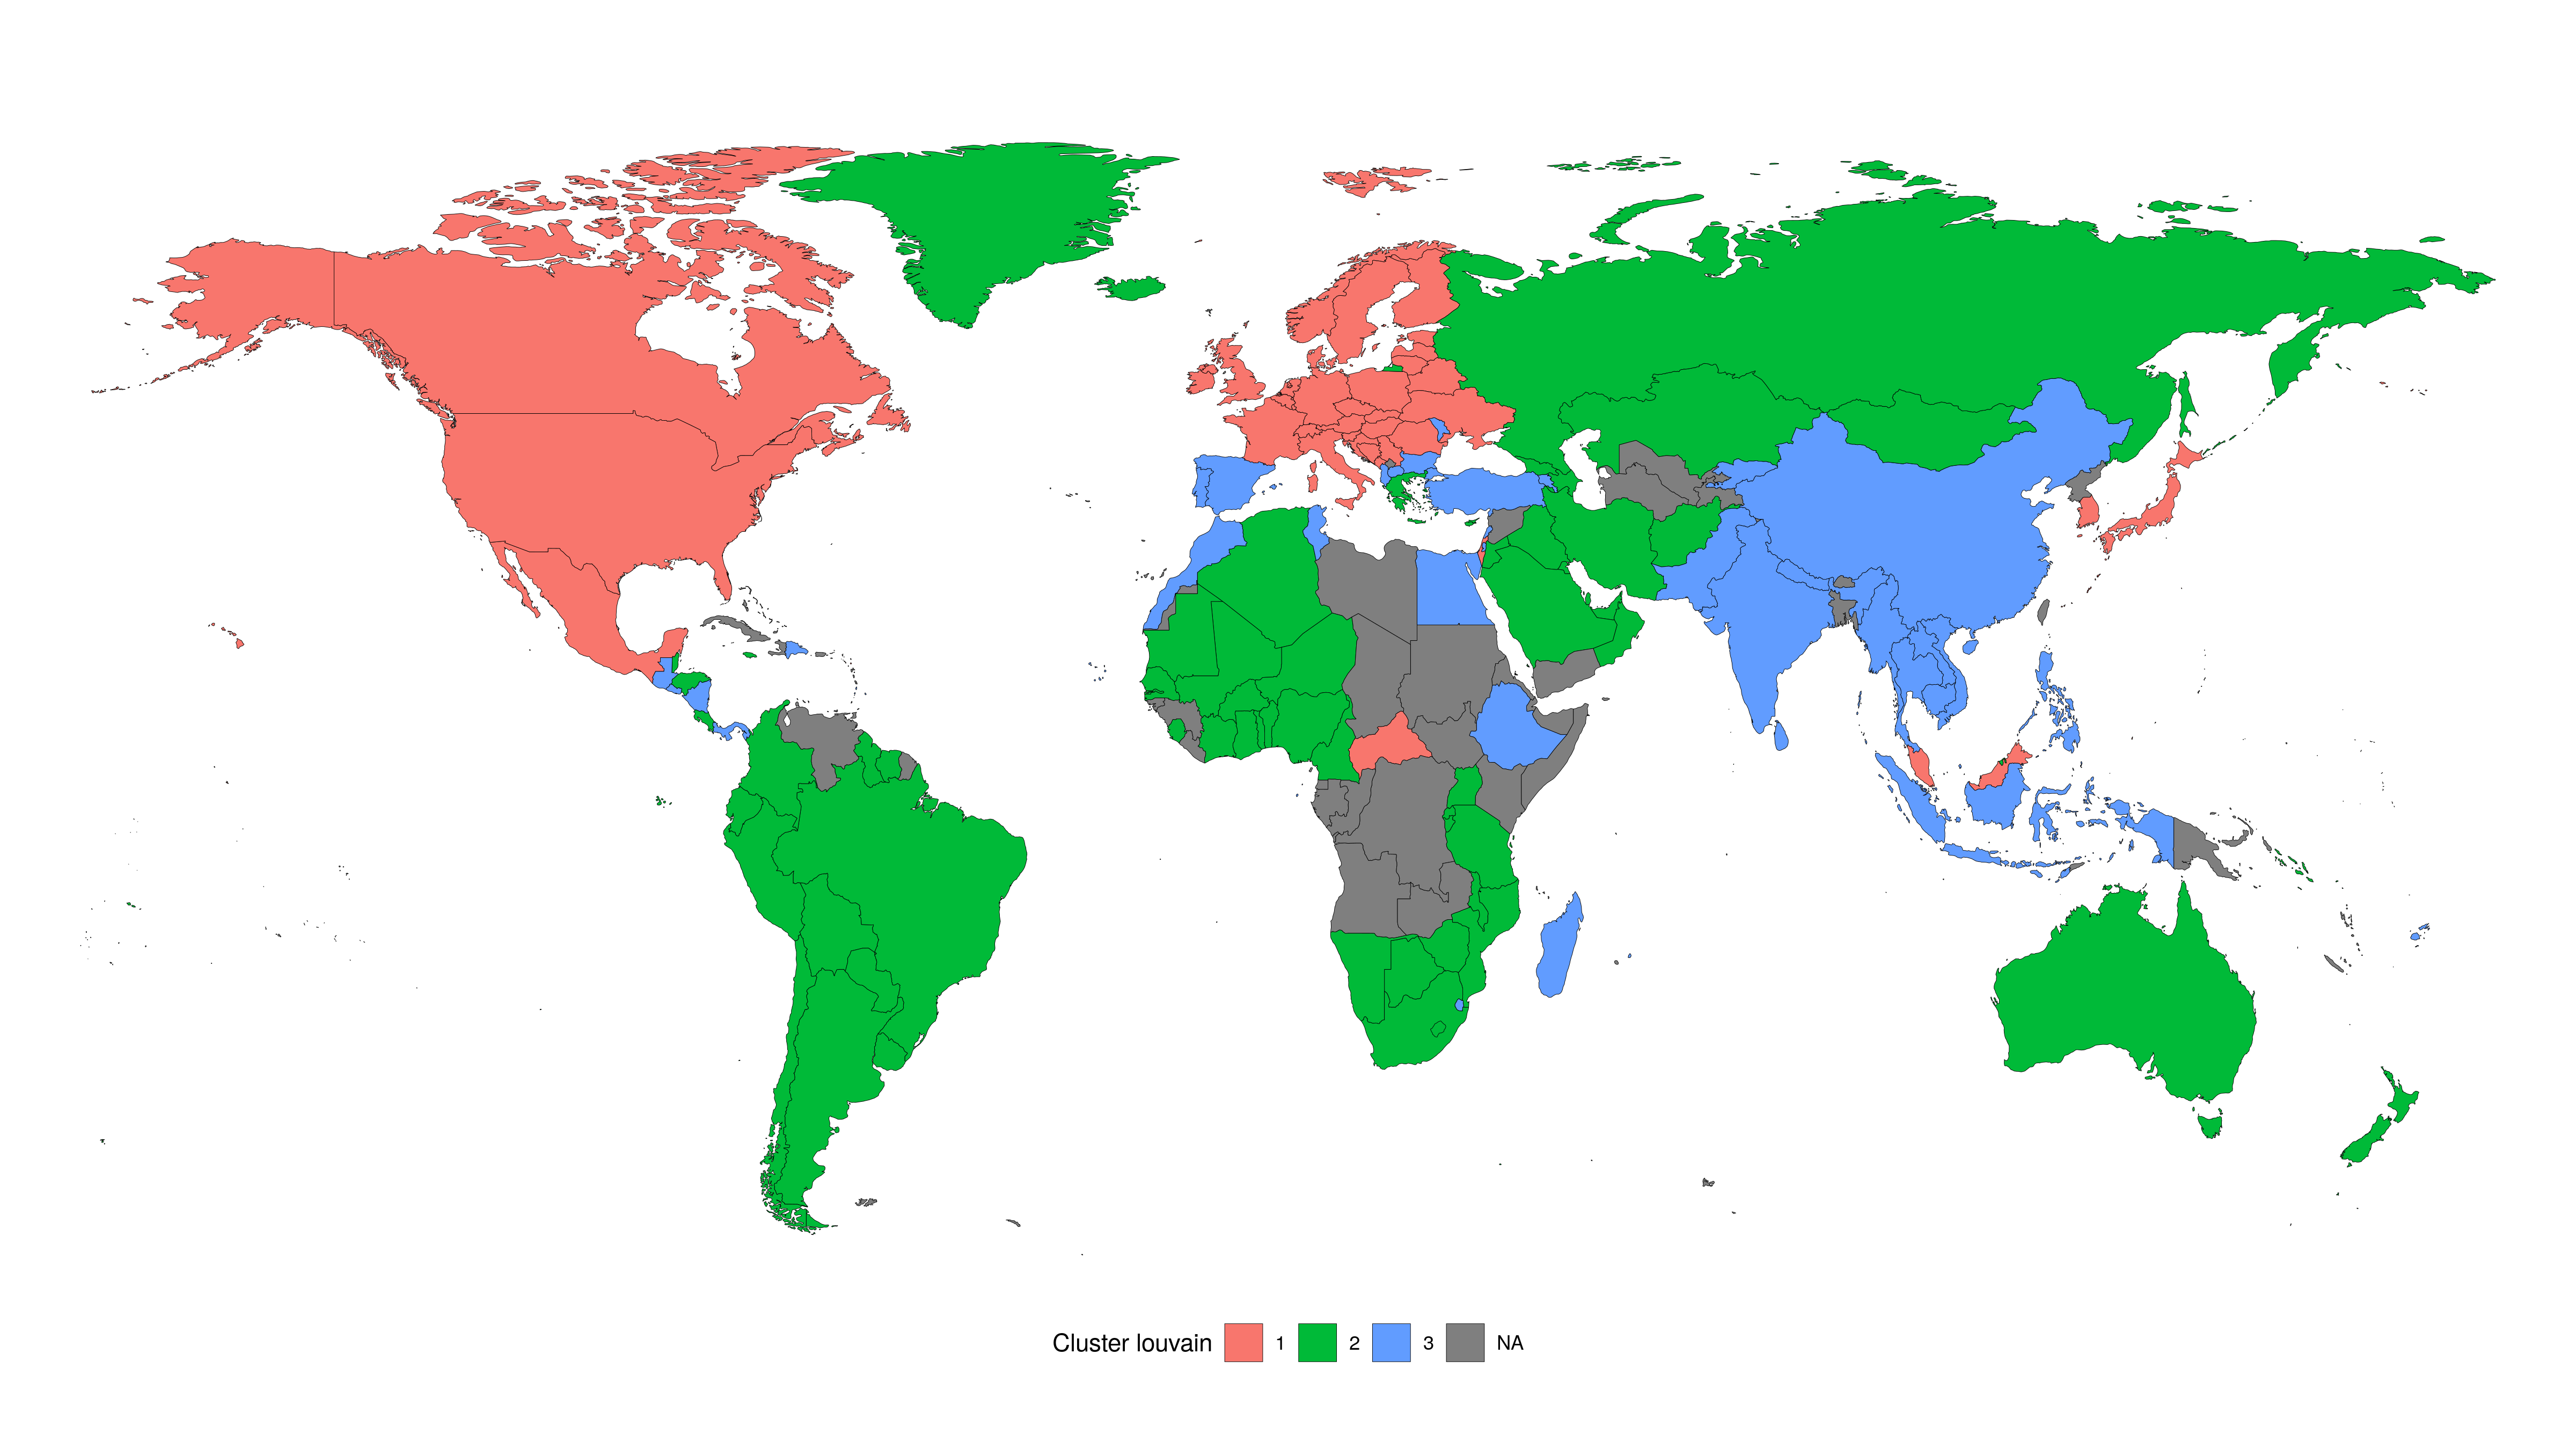
\includegraphics[width=\linewidth]{mapa_projection_louvain}}
	\subfigure[Cluster Walktrap]{\label{fig:mapas_proyeccion_2}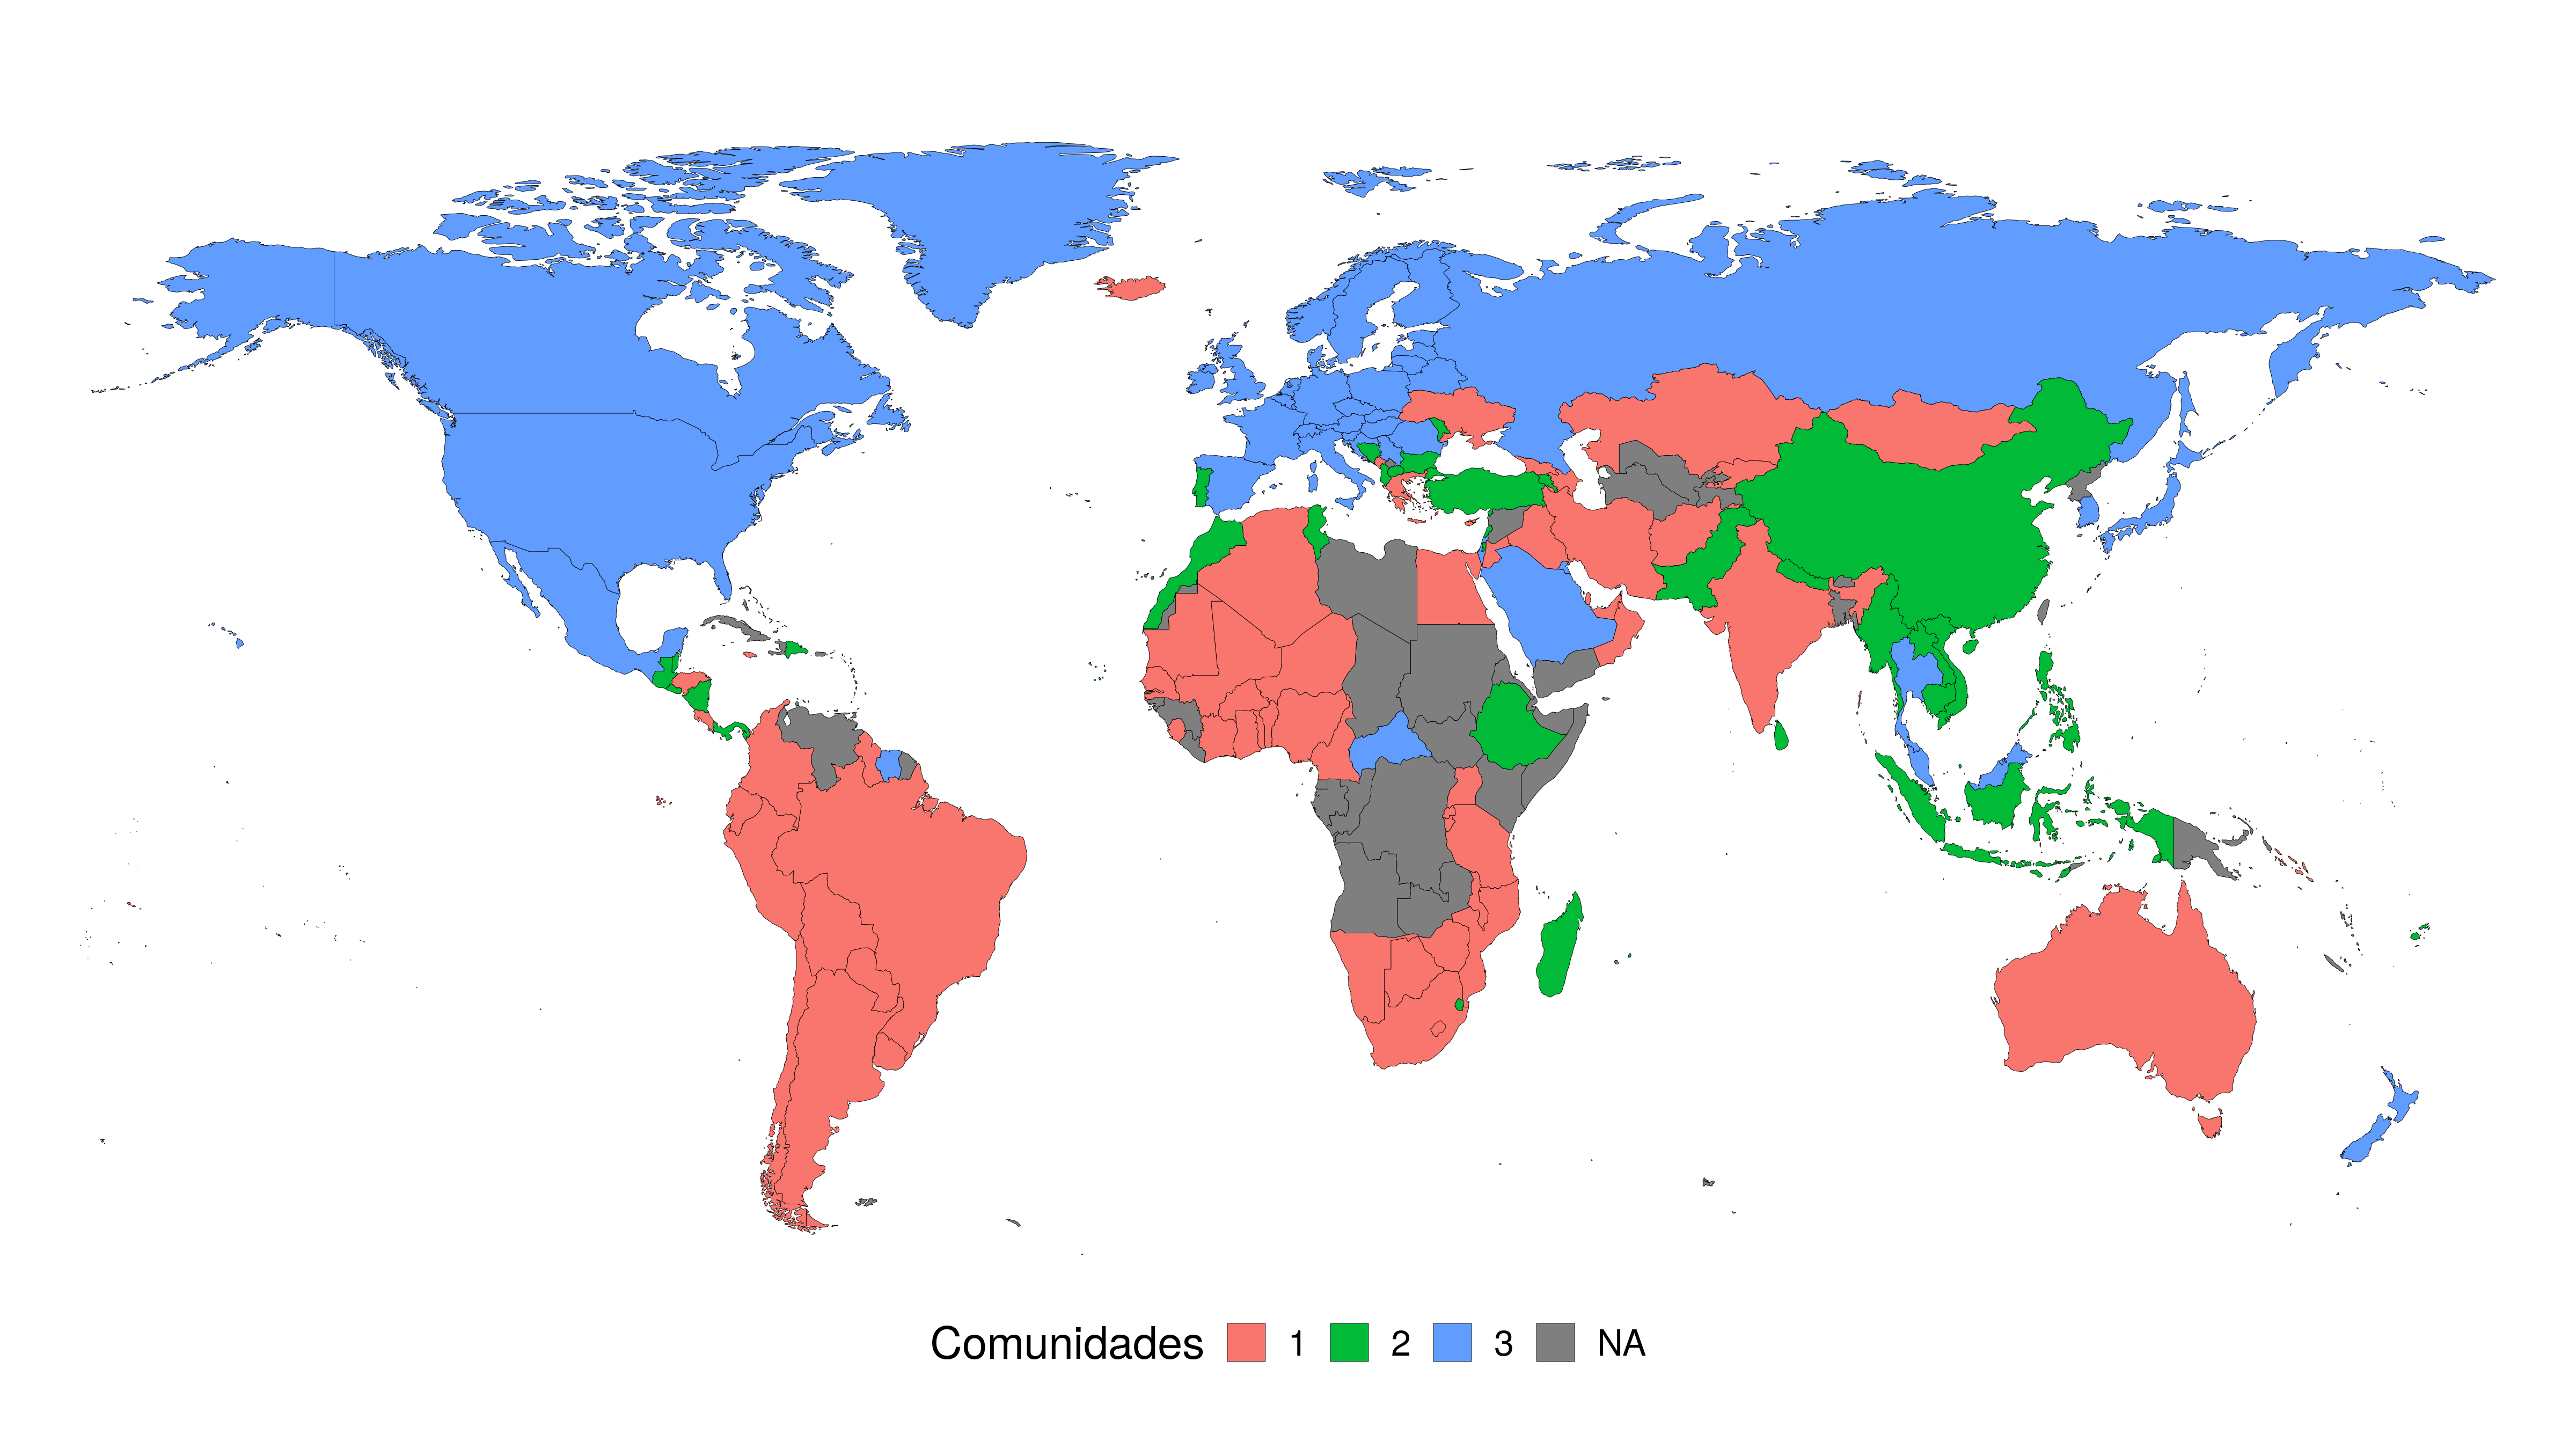
\includegraphics[width=\linewidth]{mapa_projection_walktrap}}
	\caption{Proyección países. Exportaciones 2016}
	\label{fig:mapas_proyeccion}
\end{figure}

Para comparar los resultados obtenidos, en la figura \ref{fig:mapa_comercio_agregado} se muestra los clusters de Louvain para el comercio agregado a nivel países (ver capítulo \ref{sec:agregado}). La imagen que se obtiene de las comunidades es muy distinta:

\begin{itemize}
	\item La primera comunidad esta compuesta por el contiente americano y Mongolia.
	\item La segunda comunidad esta compuesta por medio oriente, excepto Israel, y parte de África del norte.
	\item A la tercer comunidad pertenecen Europa, excepto el Reino Unido, Bélgica y Portugual.
	\item El cuarto cluster se corresponde con el sudeste asiático y África noroccidental.
	\item La quinta comunidad se corresponde con el África austral.
	\item Aunque difícil de reconocer en el mapa, el último cluster esta compuesto por Palau, Andorra, Guam y Micronesia.
\end{itemize}

Aquí se pueden apreciar los regionalismos comerciales, y el rol que la distancia geográfica juega en el comercio internacional \citep{Head2014}. De las figuras \ref{fig:mapas_proyeccion} y \ref{fig:mapa_comercio_agregado} se puede concluir que las distintas representaciones de la información del comercio internacional, según socios comerciales o similitud en la estructura productiva, logran dar con distintas expresiones del sistema económico mundial, siendo todas estas parte de un mismo fenómeno.

\begin{figure}
	\centering	
	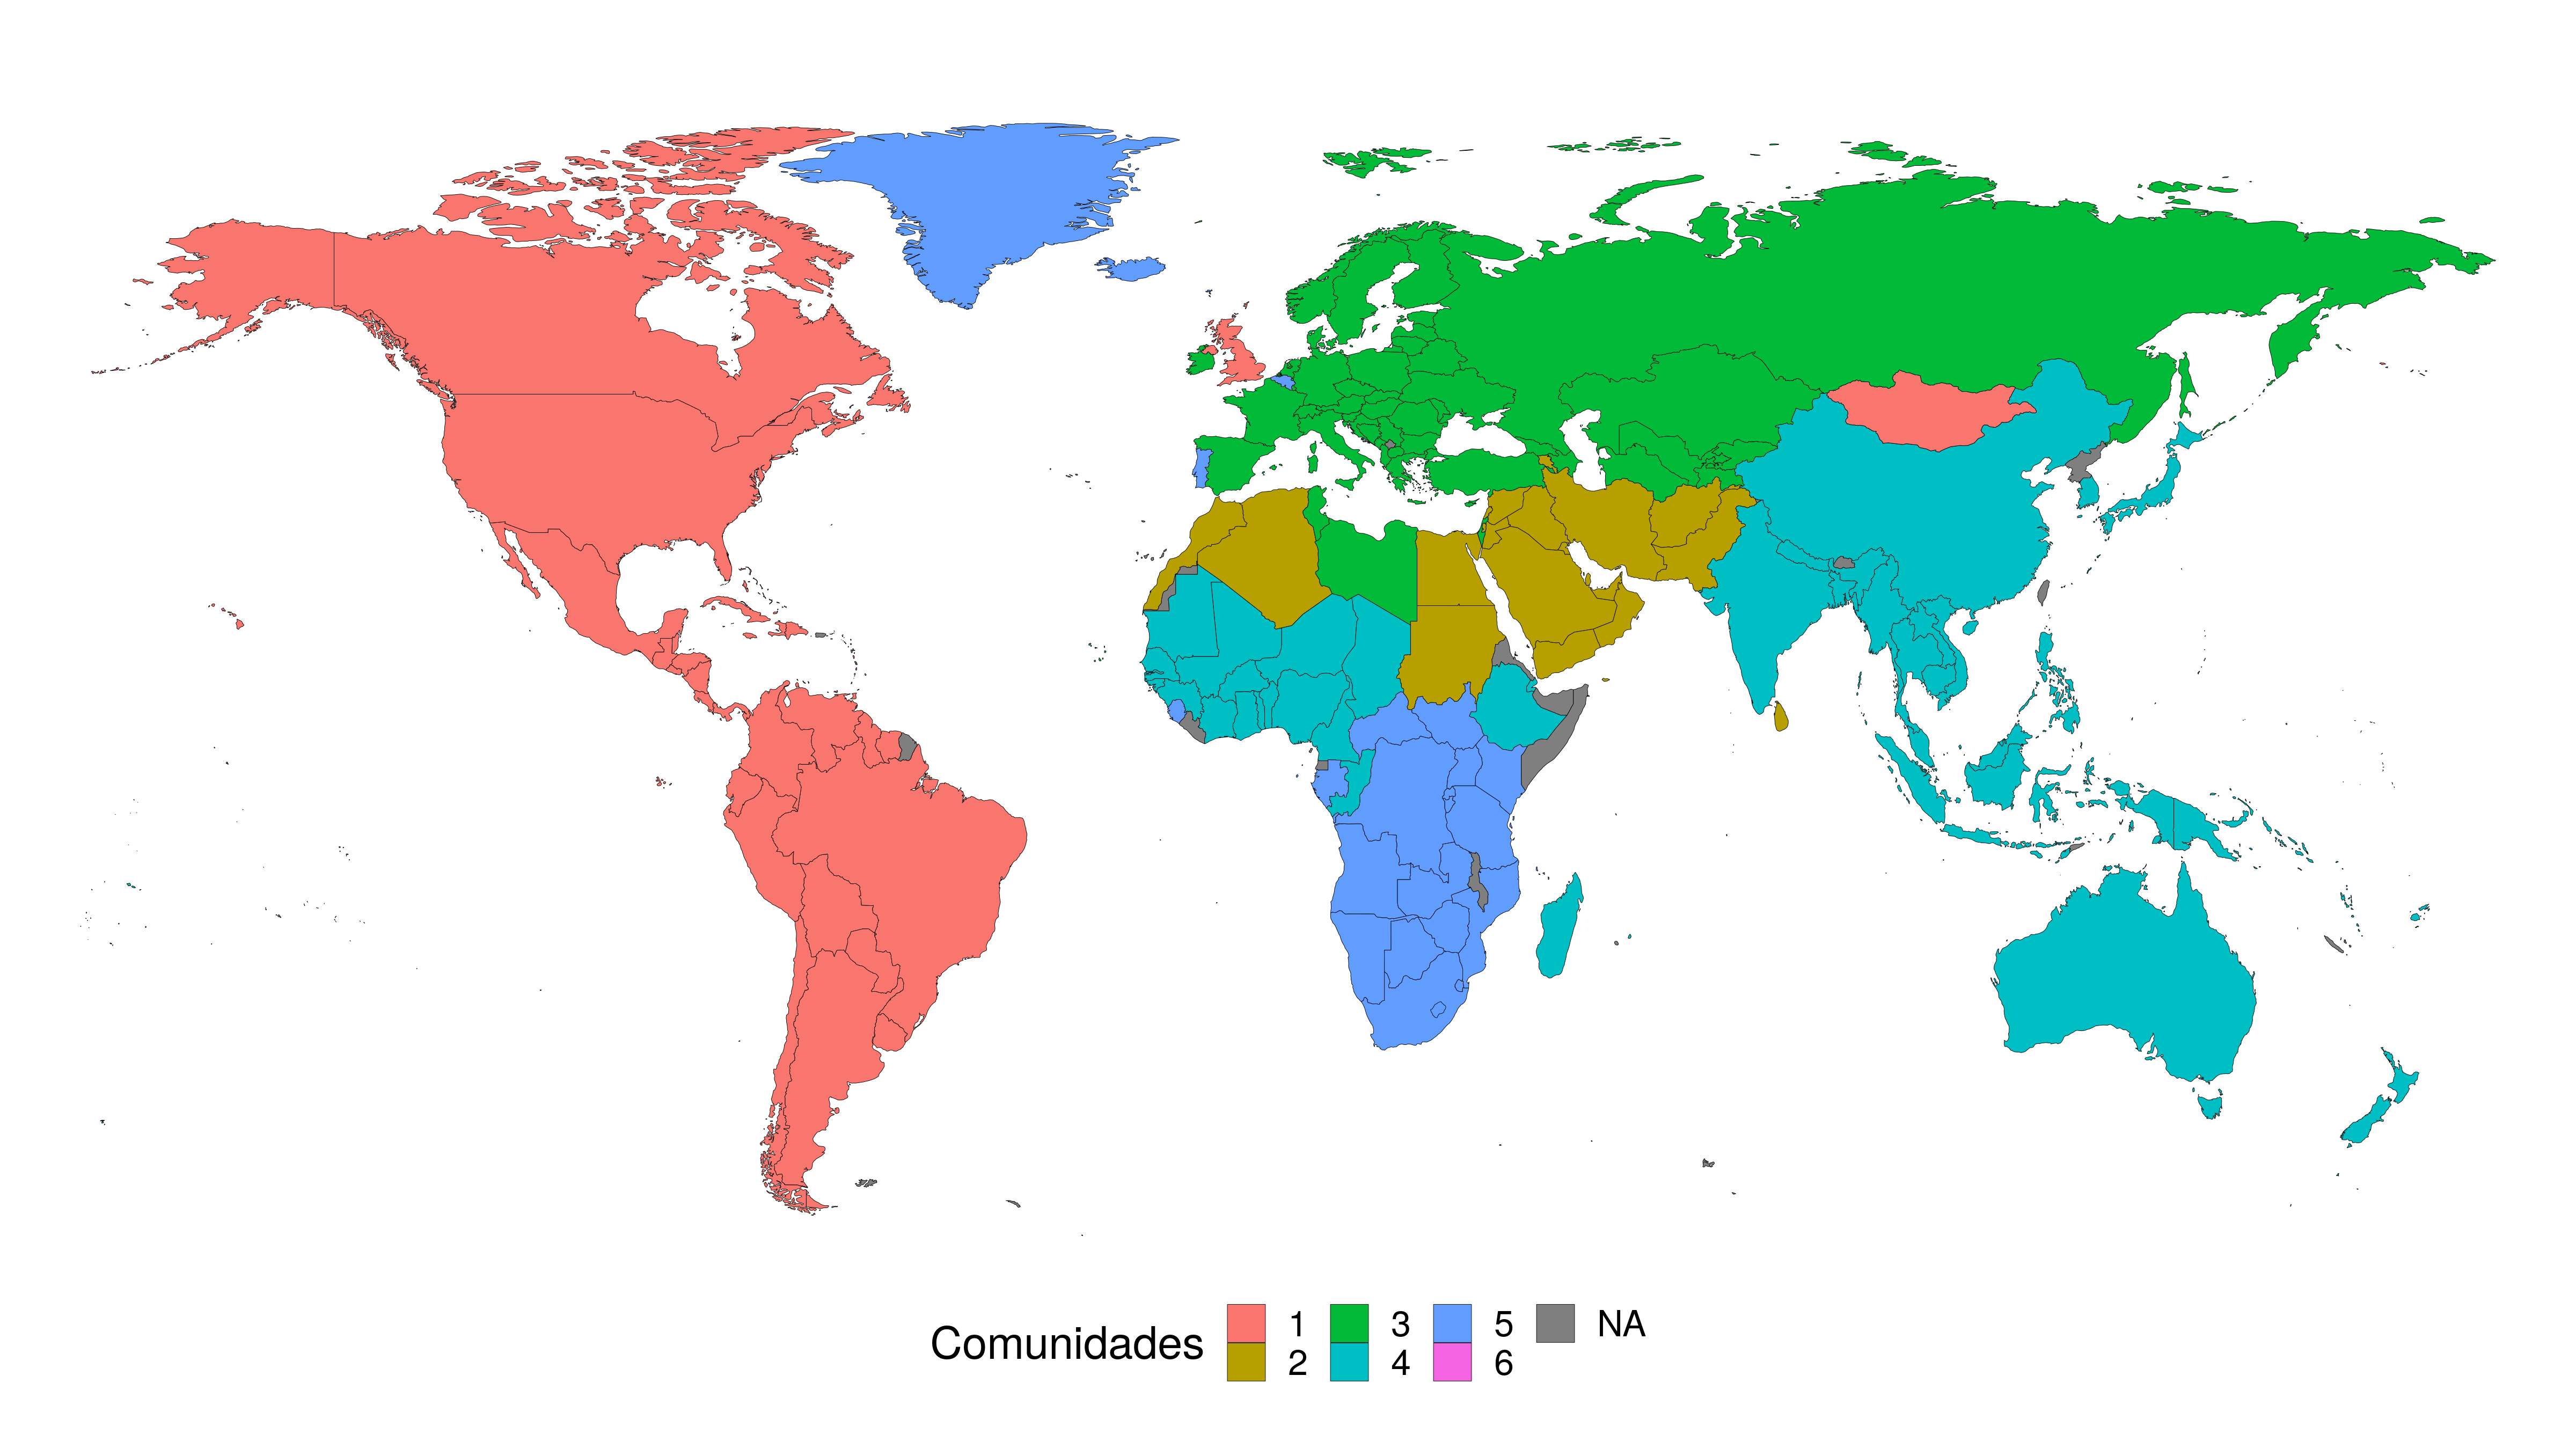
\includegraphics[width=\linewidth]{mapa_louvain}
	\caption{Cluster Louvain. Comercio agregado. Exportaciones 2016}
	\label{fig:mapa_comercio_agregado}
\end{figure}

\subsubsection{Espacio de productos}

Como se mencionó en la metodología, para analizar las relaciones entre los productos se toma como base a \cite{Hidalgo2009} y su concepto de \textit{Espacio de productos}. el mismo se define a partir de un concepto de distancia, definido como \textit{proximidad} analizado en la sección correspondiente de la metodología. Esto se aplico sobre el RCA promedio del período 1996-2017, para SITC desagregado a 4 dígitos. Para realizar una primera caracterización del espacio de productos, en \ref{fig:proximity} se muestra el mapa de calor. En \ref{fig:proximity_1} los productos se encuentran ordenados alfabéticamente según su nomenclador SITC. En \ref{fig:proximity_2} la matriz se ordena a partir de realizar un clustering jerárquico. Dado que algunos pares de productos tienen una proximidad igual a cero, al calcular la matriz de distancias estos pares tienen distancia infinita, por lo que la misma se reemplaza por un valor alto fuera de rango.

Más allá de este ajuste para realizar el clustering, en \ref{fig:proximity_2} se mantienen los valores originales para todos los $\phi_{ij}$. Las diferencias que se observan entre ambas figuras dan cuenta que el nomenclador SITC no mantiene el ordenamiento propio del espacio de productos dada la similitud en términos de proximidad. Este resultado refuerza la motivación del nomenclador construido a partir de \textit{Latent Dirichlet Allocation Models} propuesto en la sección precedente. 

\begin{figure}
	\centering
	\subfigure[Ordenamiento SITC]{\label{fig:proximity_1}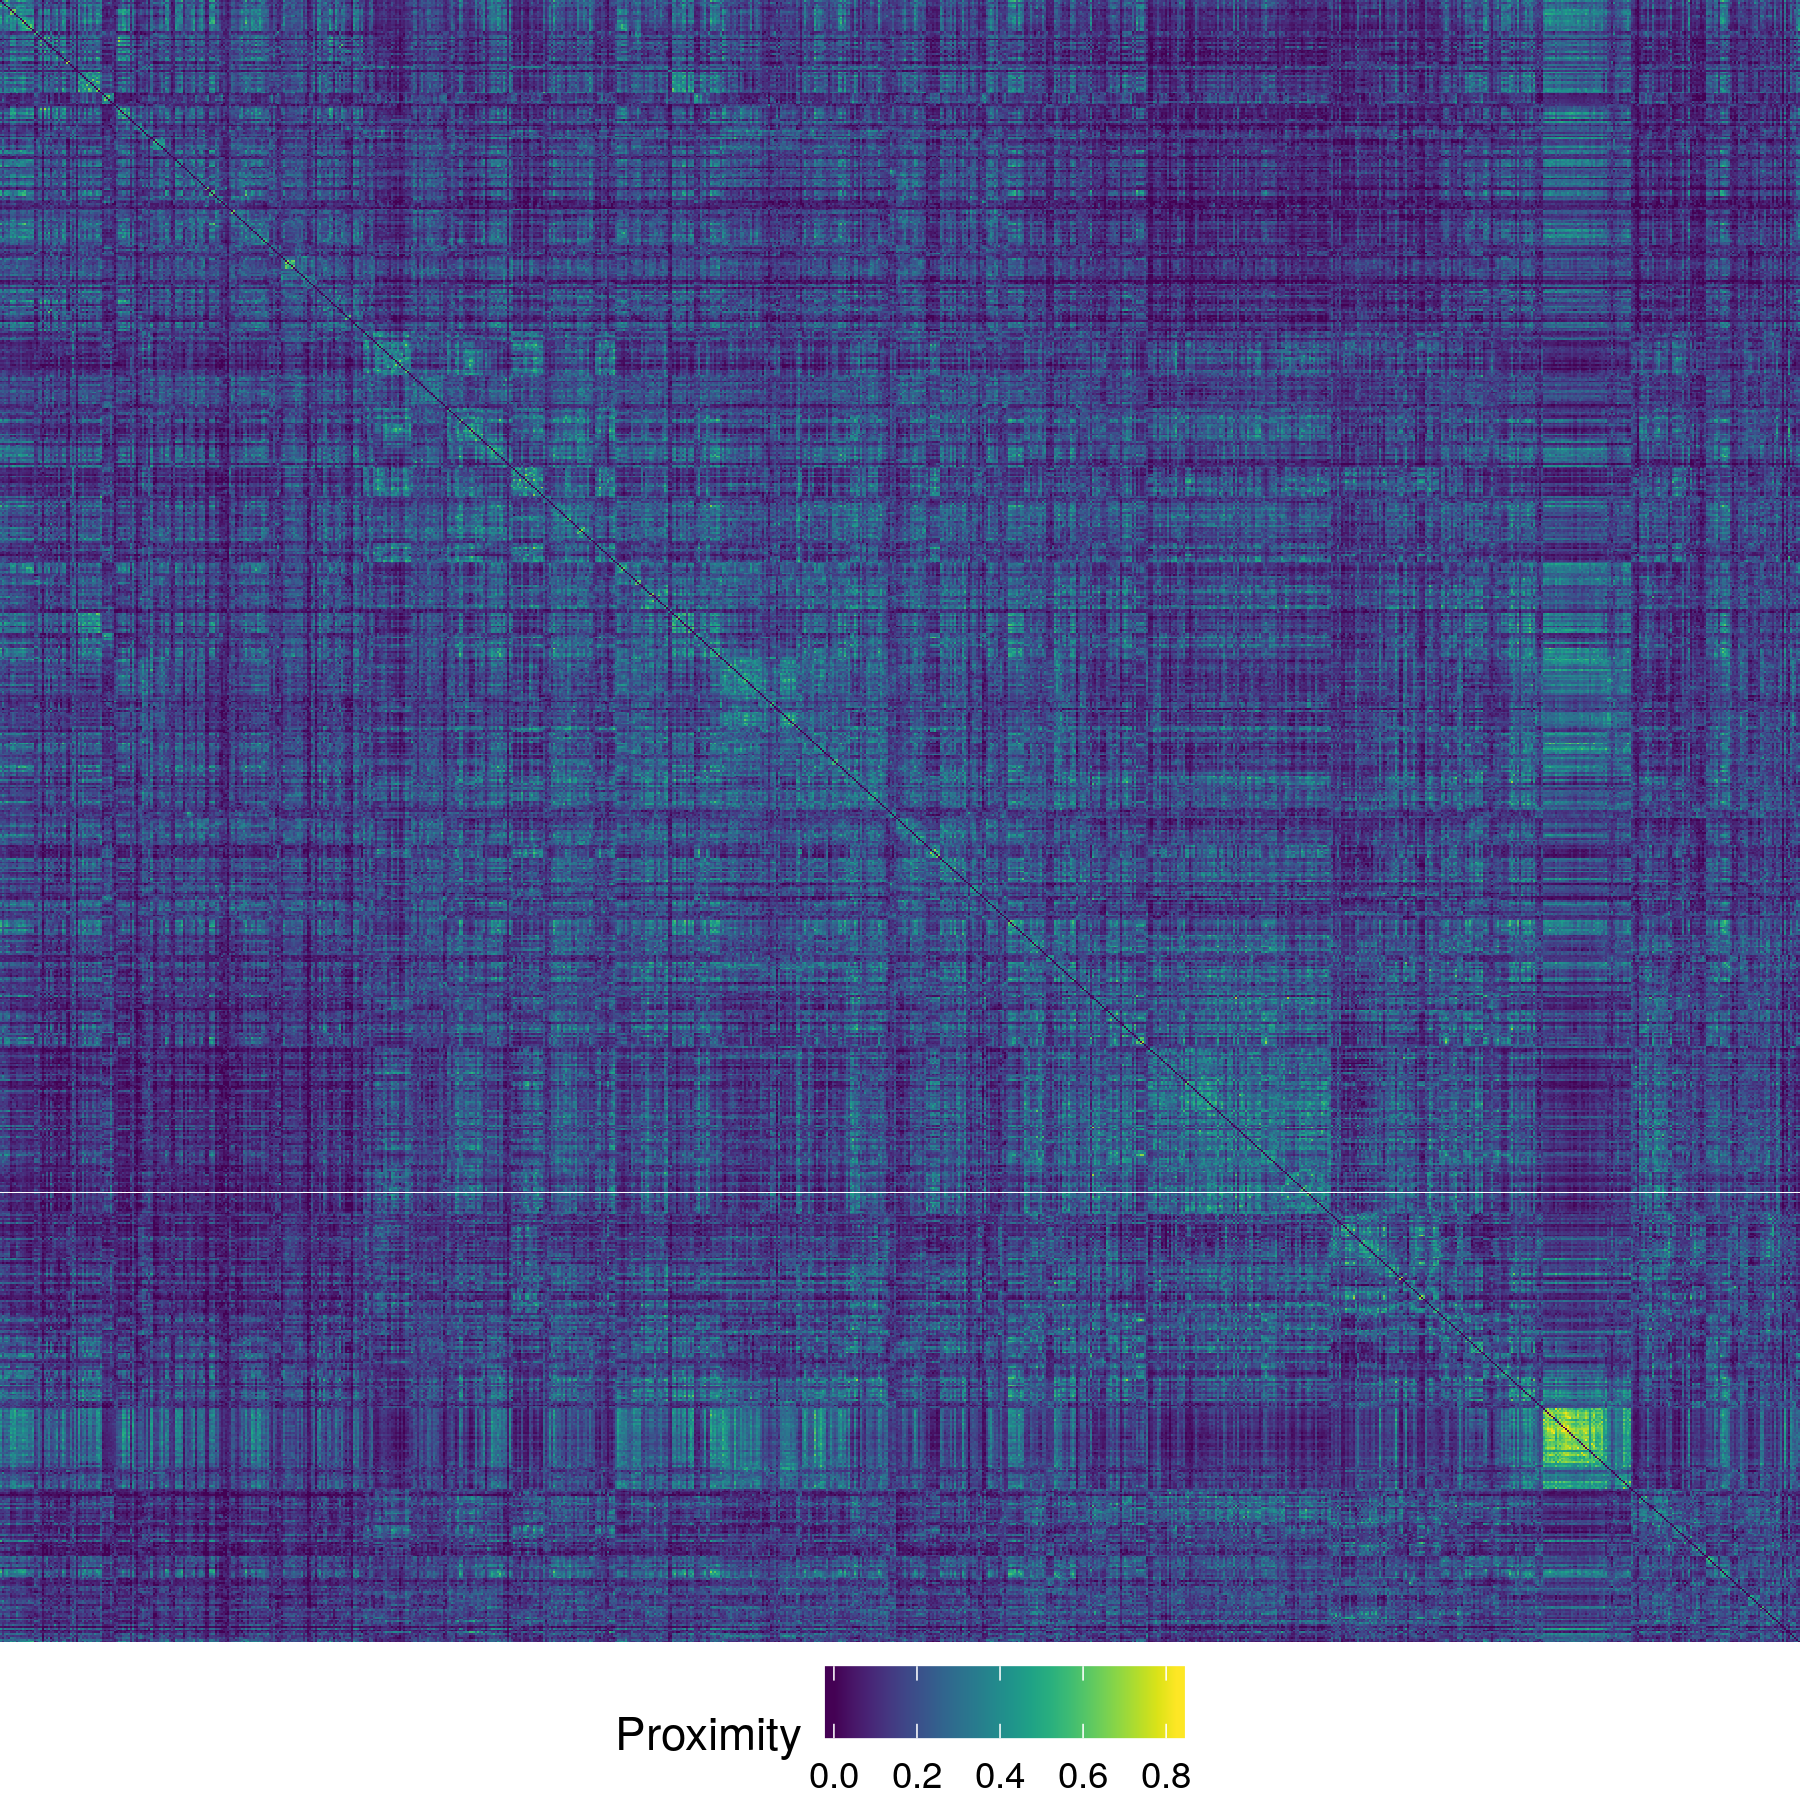
\includegraphics[width=.45\linewidth]{heatmap_prox_sitcOrd}}
	\subfigure[Ordenamiento Clustering jerárquico]{\label{fig:proximity_2}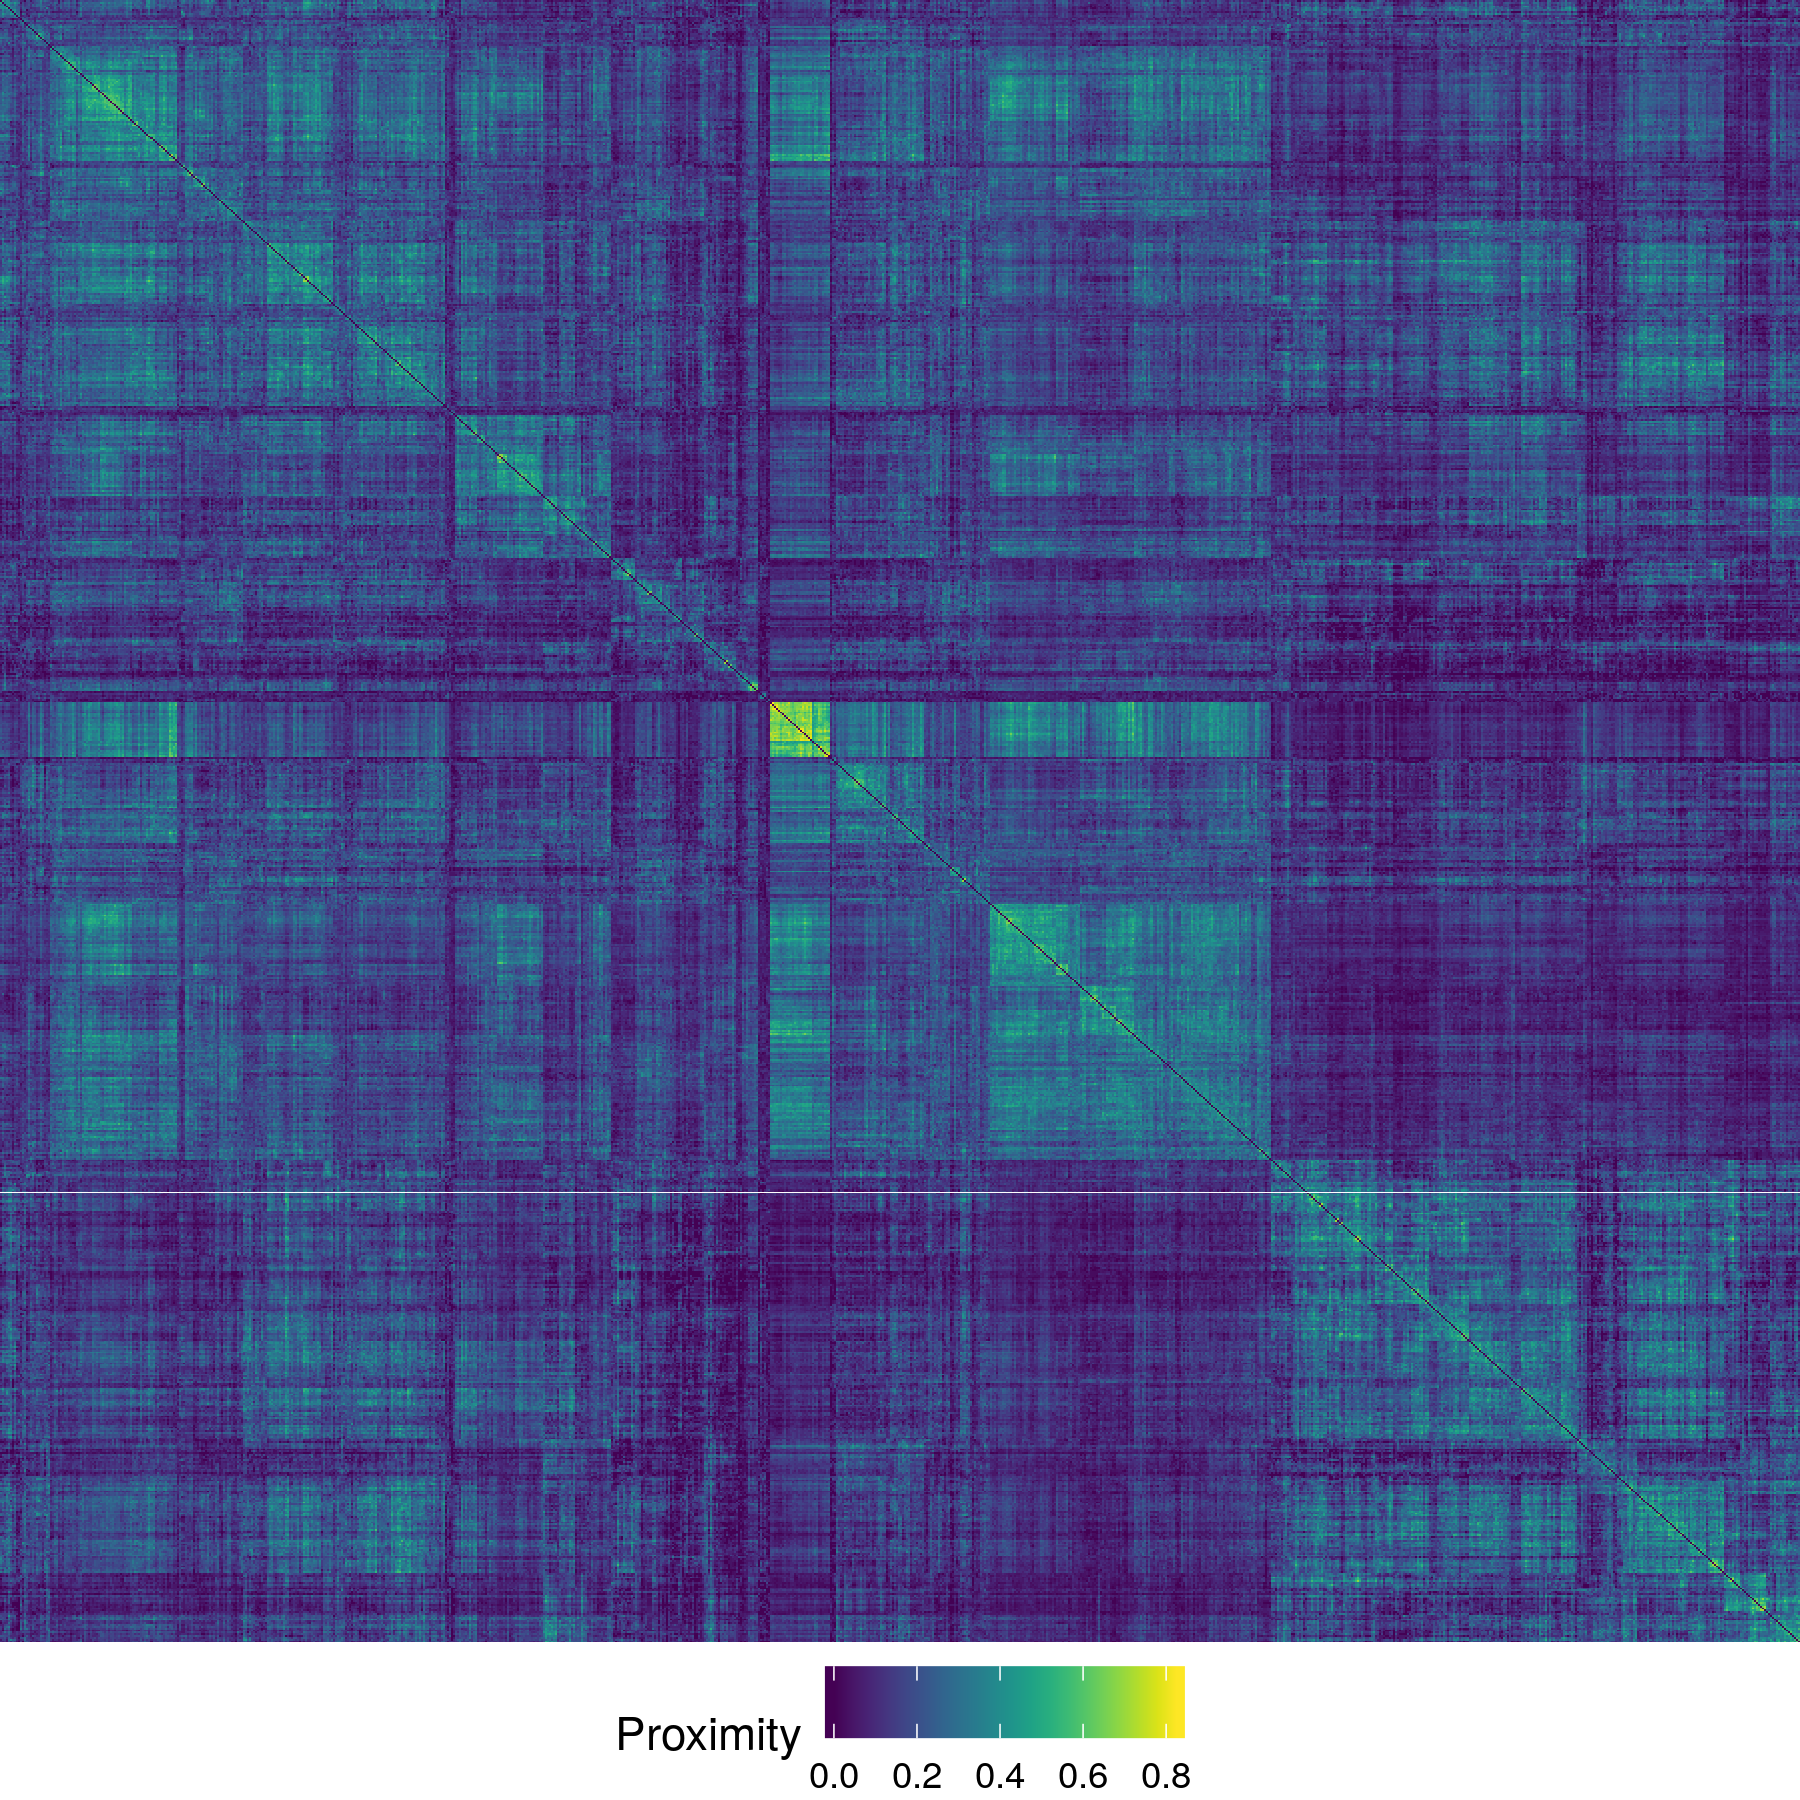
\includegraphics[width=.45\linewidth]{heatmap_prox_ClustOrd}}
	\caption{Heatmap proximidad. Espacio de productos. Exportaciones. Promedio 1996-2017}
	\label{fig:proximity}
\end{figure}

En ambos mapas de calor se puede observar que existe un pequeño conjunto de productos de muy alta proximidad. Para observar dicho fenómeno, en la tabla \ref{table:similarity} se destacan los diez pares productos de mayor proximidad, y su descripción a cuatro dígitos. Como se observa, todos ellos son productos textiles, algunos de ellos incluso compartiendo descripción a cuatro dígitos. Los procesos productivos para realizar estas mercancías son muy similares y requieren básicamente de los mismos insumos, maquinaria y mano de obra, lo cual explica su similitud. 


\begin{table}[]
	\begin{tabular}{|r|l|l|l|l|}
		\hline
		\textbf{Sim}               & $SITC_1$ & \textbf{Descripción}                                                                                                     & $SITC_2$ & \textbf{Descripción}                                                                                                     \\ \hline
		0.82                       & 8438     & underwear,nightwear etc.                                                                                                 & 8448     & underwear, nightwear etc                                                                                                 \\ \hline
		0.82                       & 8425     & \begin{tabular}[c]{@{}l@{}}skirts and divided skirts,\\ women's or girls',\\ of textile materials, not k\end{tabular}    & 8427     & \begin{tabular}[c]{@{}l@{}}blouses,\\ shirts and shirt-blouses,\\ women's or girls', \\ of textile material\end{tabular} \\ \hline
		0.82                       & 8416     & underwear,nightwear etc.                                                                                                 & 8428     & underwear,nightwear etc.                                                                                                 \\ \hline
		0.81                       & 8424     & \begin{tabular}[c]{@{}l@{}}dresses,\\ women's or girls',\\ of textile materials,\\ notted or crochete\end{tabular}       & 8425     & \begin{tabular}[c]{@{}l@{}}skirts and divided skirts,\\ women's or girls',\\ of textile materials, not k\end{tabular}    \\ \hline
		0.80                       & 8427     & \begin{tabular}[c]{@{}l@{}}blouses,\\ shirts and shirt-blouses,\\ women's or girls', \\ of textile material\end{tabular} & 8424     & \begin{tabular}[c]{@{}l@{}}dresses,\\ women's or girls',\\ of textile materials,\\ notted or crochete\end{tabular}       \\ \hline
		0.80                       & 8425     & shirts and shirt-blouses,                                                                                                & 8426     & \begin{tabular}[c]{@{}l@{}}trousers, \\ bib and brace overalls,\\ breeches and shorts,\\ women's or girls\end{tabular}   \\ \hline
		0.80                       & 8428     & women's or girls',                                                                                                       & 8448     & underwear, nightwear etc                                                                                                 \\ \hline
		0.79                       & 8411     & of textile material                                                                                                      & 8421     & overcoats,oth.coats etc.                                                                                                 \\ \hline
		0.79                       & 8415     & shirts                                                                                                                   & 8426     & \begin{tabular}[c]{@{}l@{}}trousers, \\ bib and brace overalls,\\ breeches and shorts,\\ women's or girls\end{tabular}   \\ \hline
		\multicolumn{1}{|l|}{0.79} & 8426     & \begin{tabular}[c]{@{}l@{}}trousers, \\ bib and brace overalls,\\ breeches and shorts,\\ women's or girls\end{tabular}   & 8427     & \begin{tabular}[c]{@{}l@{}}blouses,\\ shirts and shirt-blouses,\\ women's or girls', \\ of textile material\end{tabular} \\ \hline
	\end{tabular}
\caption{Top 10 pares de productos más similares}
\label{table:similarity}
\end{table}


Teniendo presente lo anterior, se utilizó la inversa de la matriz de similaridad como una matriz de distancias para calcular clusters con mediante el método \textit{Partition around medioids}. A su vez, con estos datos se reconstruyó el grafo de productos utilizando una versión modificada de la matriz de proximidad como matriz de adyacencia del grafo. Específicamente, para aquellos productos con una proximidad menor a 0.5 se anuló la métrica: 


$$
\phi_{ij} = 
\begin{cases} 
\phi_{ij} & si \ \phi_{ij}>0.5 \\
0 & si \ \phi_{ij}<0.5
\end{cases}
$$

Con esta matriz de proximidad modificada se reconstruyó el grafo. En la figura \ref{fig:clustering2} se observa el componente gigante, identificando la pertenencia de cada nodo y su medioide.


\begin{figure}
	\centering	
	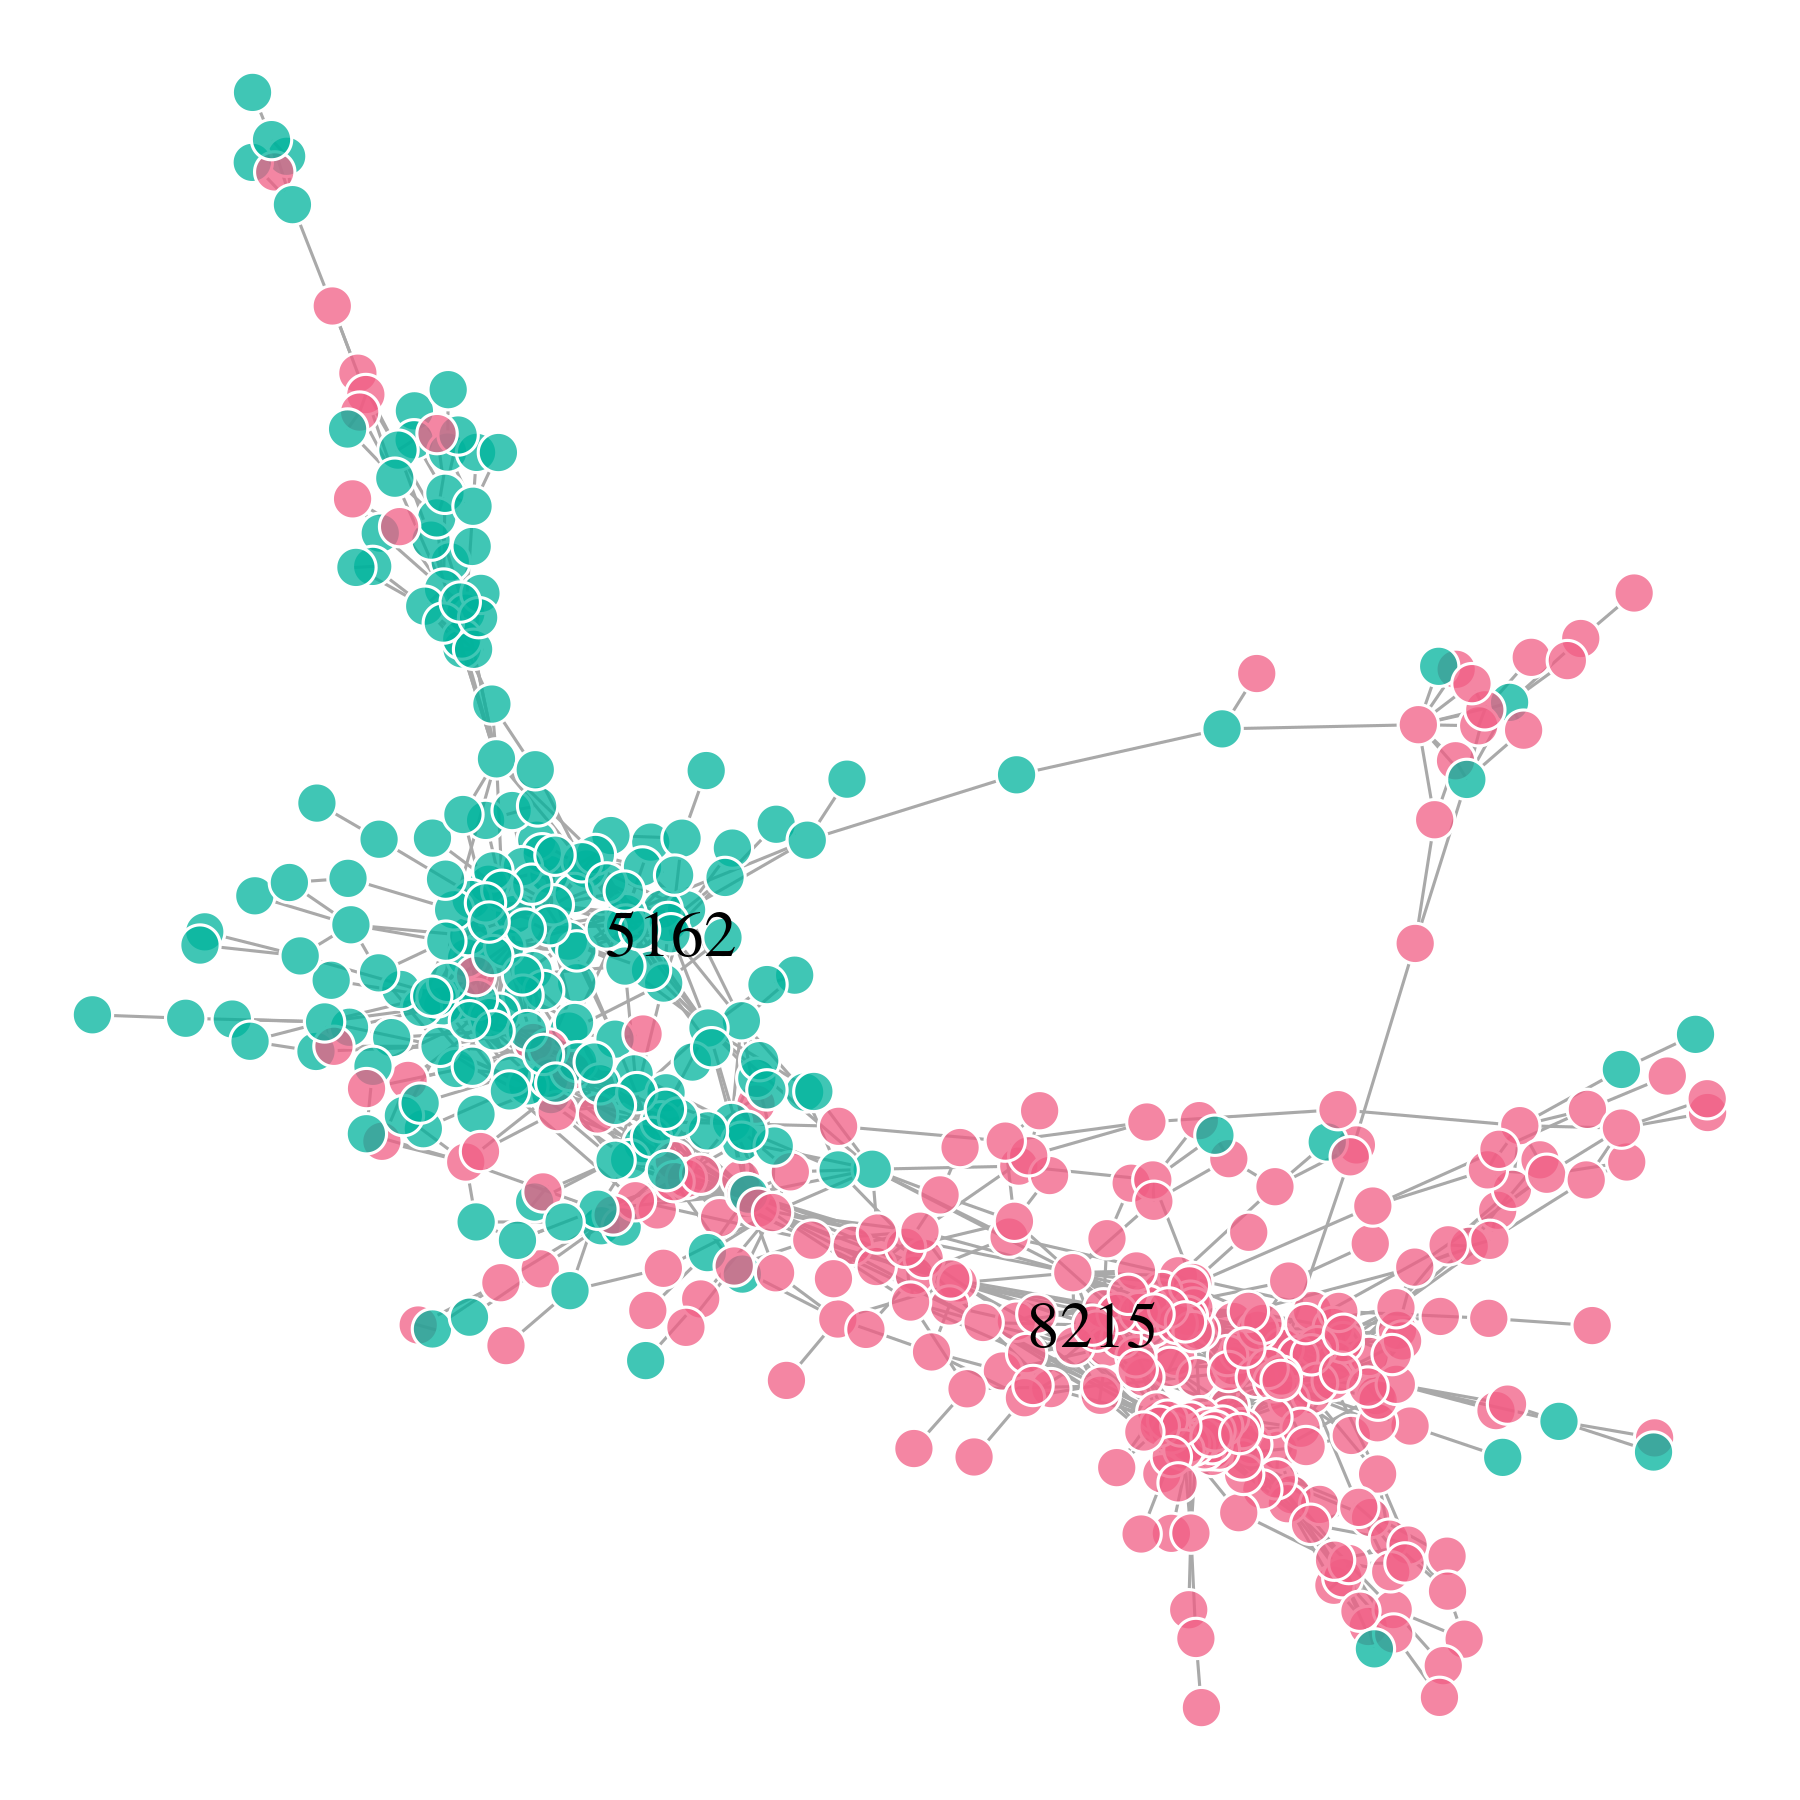
\includegraphics[width=\linewidth]{pam2_gigant}
	\caption{Componente gigante. Grafo de proximidad y clustering por K-medioides. Exportaciones. Promedio 1996-2017. 2 medioides}
	\label{fig:clustering2}
\end{figure}

En la figura \ref{fig:clustering2} se puede observar una buena separación entre ambos clusters dentro del componente gigante espacio de productos. En la tabla \ref{table:pam2} se describen los medioides. Dado que el \textit{Aldehyde} es un químico para sintetizar otros compuestos, mientras que el otro mediodide esta caracterizado por muebles de madera, podemos decir que el cluster en verde representa productos de alta complejidad, mientras que el cluster rojo representa a los productos de baja complejidad. 

\begin{table}
	\centering
	\begin{tabular}{ll}
		\hline
		medioide & Description \\ 
		\hline
		8215 & Furniture,nes,of wood \\ 
		5162 & Aldehyde,etc.fnct.cmpnds \\ 
		\hline
	\end{tabular}
	\caption{Medioides. PAM. k=2} 
	\label{table:pam2}
\end{table}


En la figura \ref{fig:clustering10} podemos observar qué sucede con 10 medioides. Aquí, si bien se mantiene una separación de los grupos en muchos casos, podemos observar que existe un solapamiento en los puntos más densos del componente gigante. Estos clusters representan a productos de alta complejidad, como componentes de maquinarias (7285), componentes químicos (5416), o productos electrónicos. Con mejor separación aparece la industria pesada (6911) y en especial equipos para el procesamiento automático de datos (7526). En la figura \ref{table:pam10} se describen los demás medioides.

\begin{figure}
	\centering	
	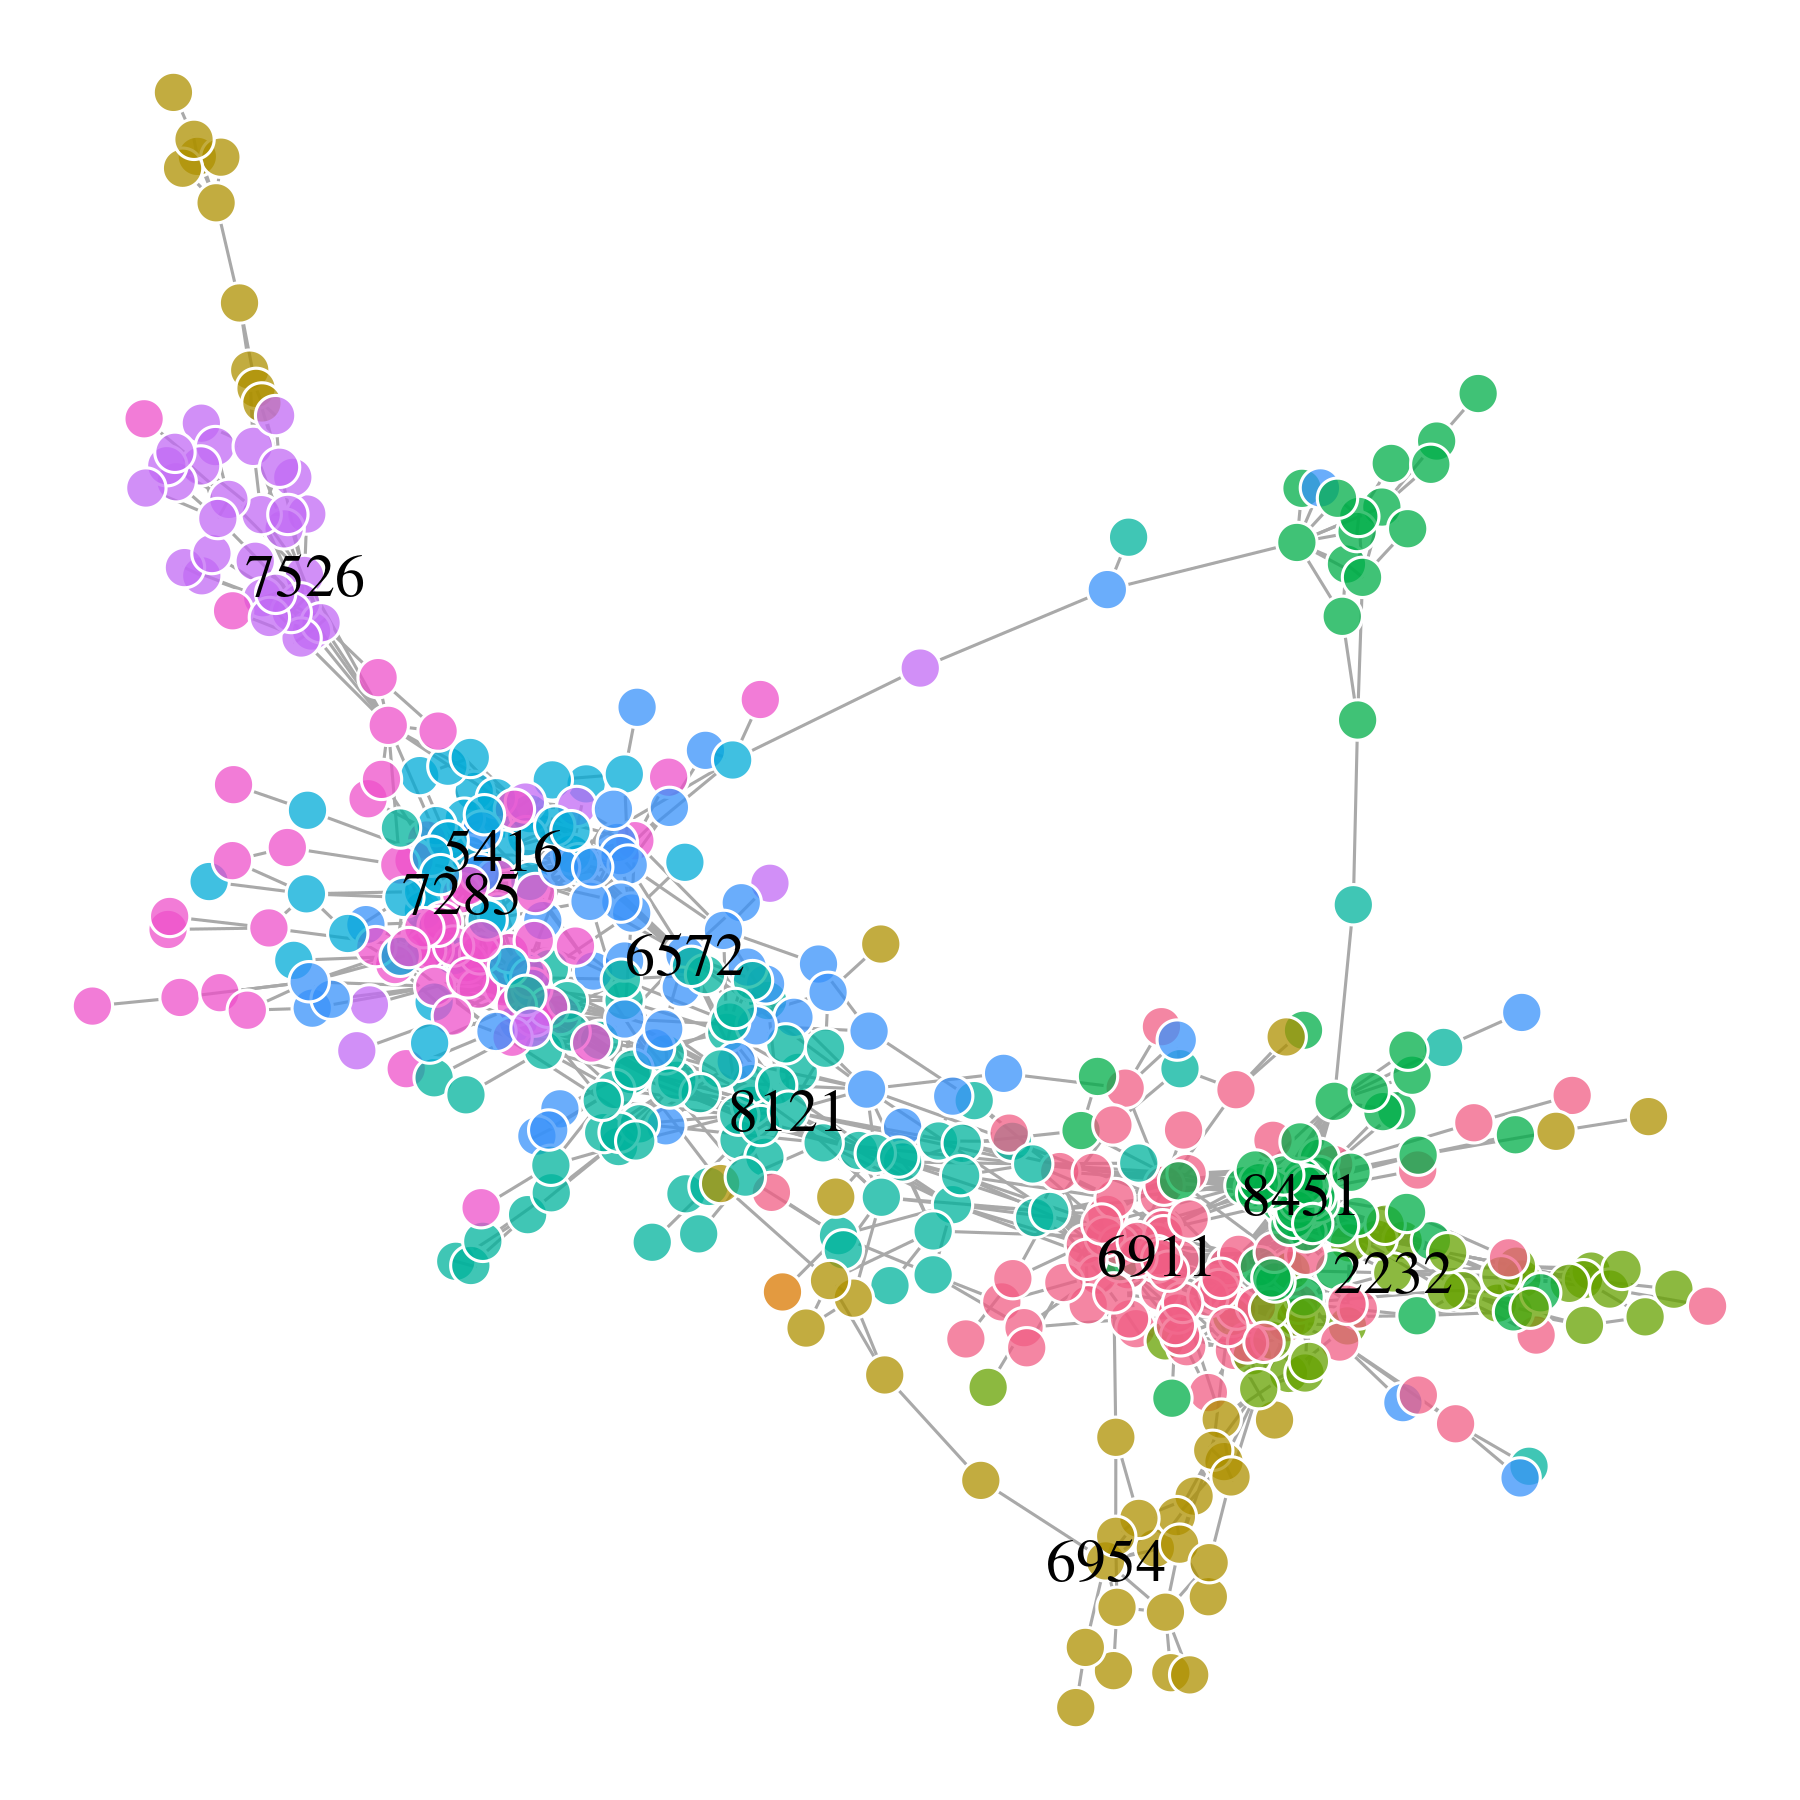
\includegraphics[width=\linewidth]{pam10_gigant}
	\caption{Componente gigante. Grafo de proximidad y clustering por K-medioides. Exportaciones. Promedio 1996-2017. 10 medioides}
	\label{fig:clustering10}
\end{figure}


\begin{table}
	\centering
	\begin{tabular}{ll}
		\hline
		medioide & Description \\ 
		\hline
		6911 & Metal structures,parts \\ 
		2831 & Copper ores and concentrates \\ 
		6954 & Hand tools,etc. nes \\ 
		2232 & Palm nuts and kernels \\ 
		8451 & Babies'garmnts,clths acc \\ 
		8121 & Boilrs.radiatrs,etc.n.el \\ 
		5416 & Glycosides; glands etc. \\ 
		6572 & Non-wovens, whether or not impregnated, coated, covered or laminated, n.e \\ 
		7526 & Input or output units for automatic data processing machines, whether or \\ 
		7285 & Parts publc wrk mach etc \\ 
		\hline
	\end{tabular}
	\caption{Medioides. PAM. k=10} 
	\label{table:pam10}
\end{table}


En la figura \ref{fig:clustering50} se analiza el caso de 50 medioides. La descripción de cada uno de ellos se encuentra en el anexo, en la tabla \ref{tabla:pam50}. Allí se fuerza lo mencionado anteriormente sobre el solapamiento en la parte más densa del grafo, siendo casi todos los medioides productos del capítulo 7, de maquinaria y equipos industriales. Es decir, es un sector del grafo de alta complejidad. Se mantiene como un cluster más o menos bien diferenciado los procesadores automáticos de datos y microcomponentes (7526, 7722), el cual se podría caracterizar como un sector de mayor complejidad que el centro del grafo. También se configura separadamente el sector de productos textiles (6562) y el de herramientas manuales (6954). 

\begin{figure}
	\centering	
	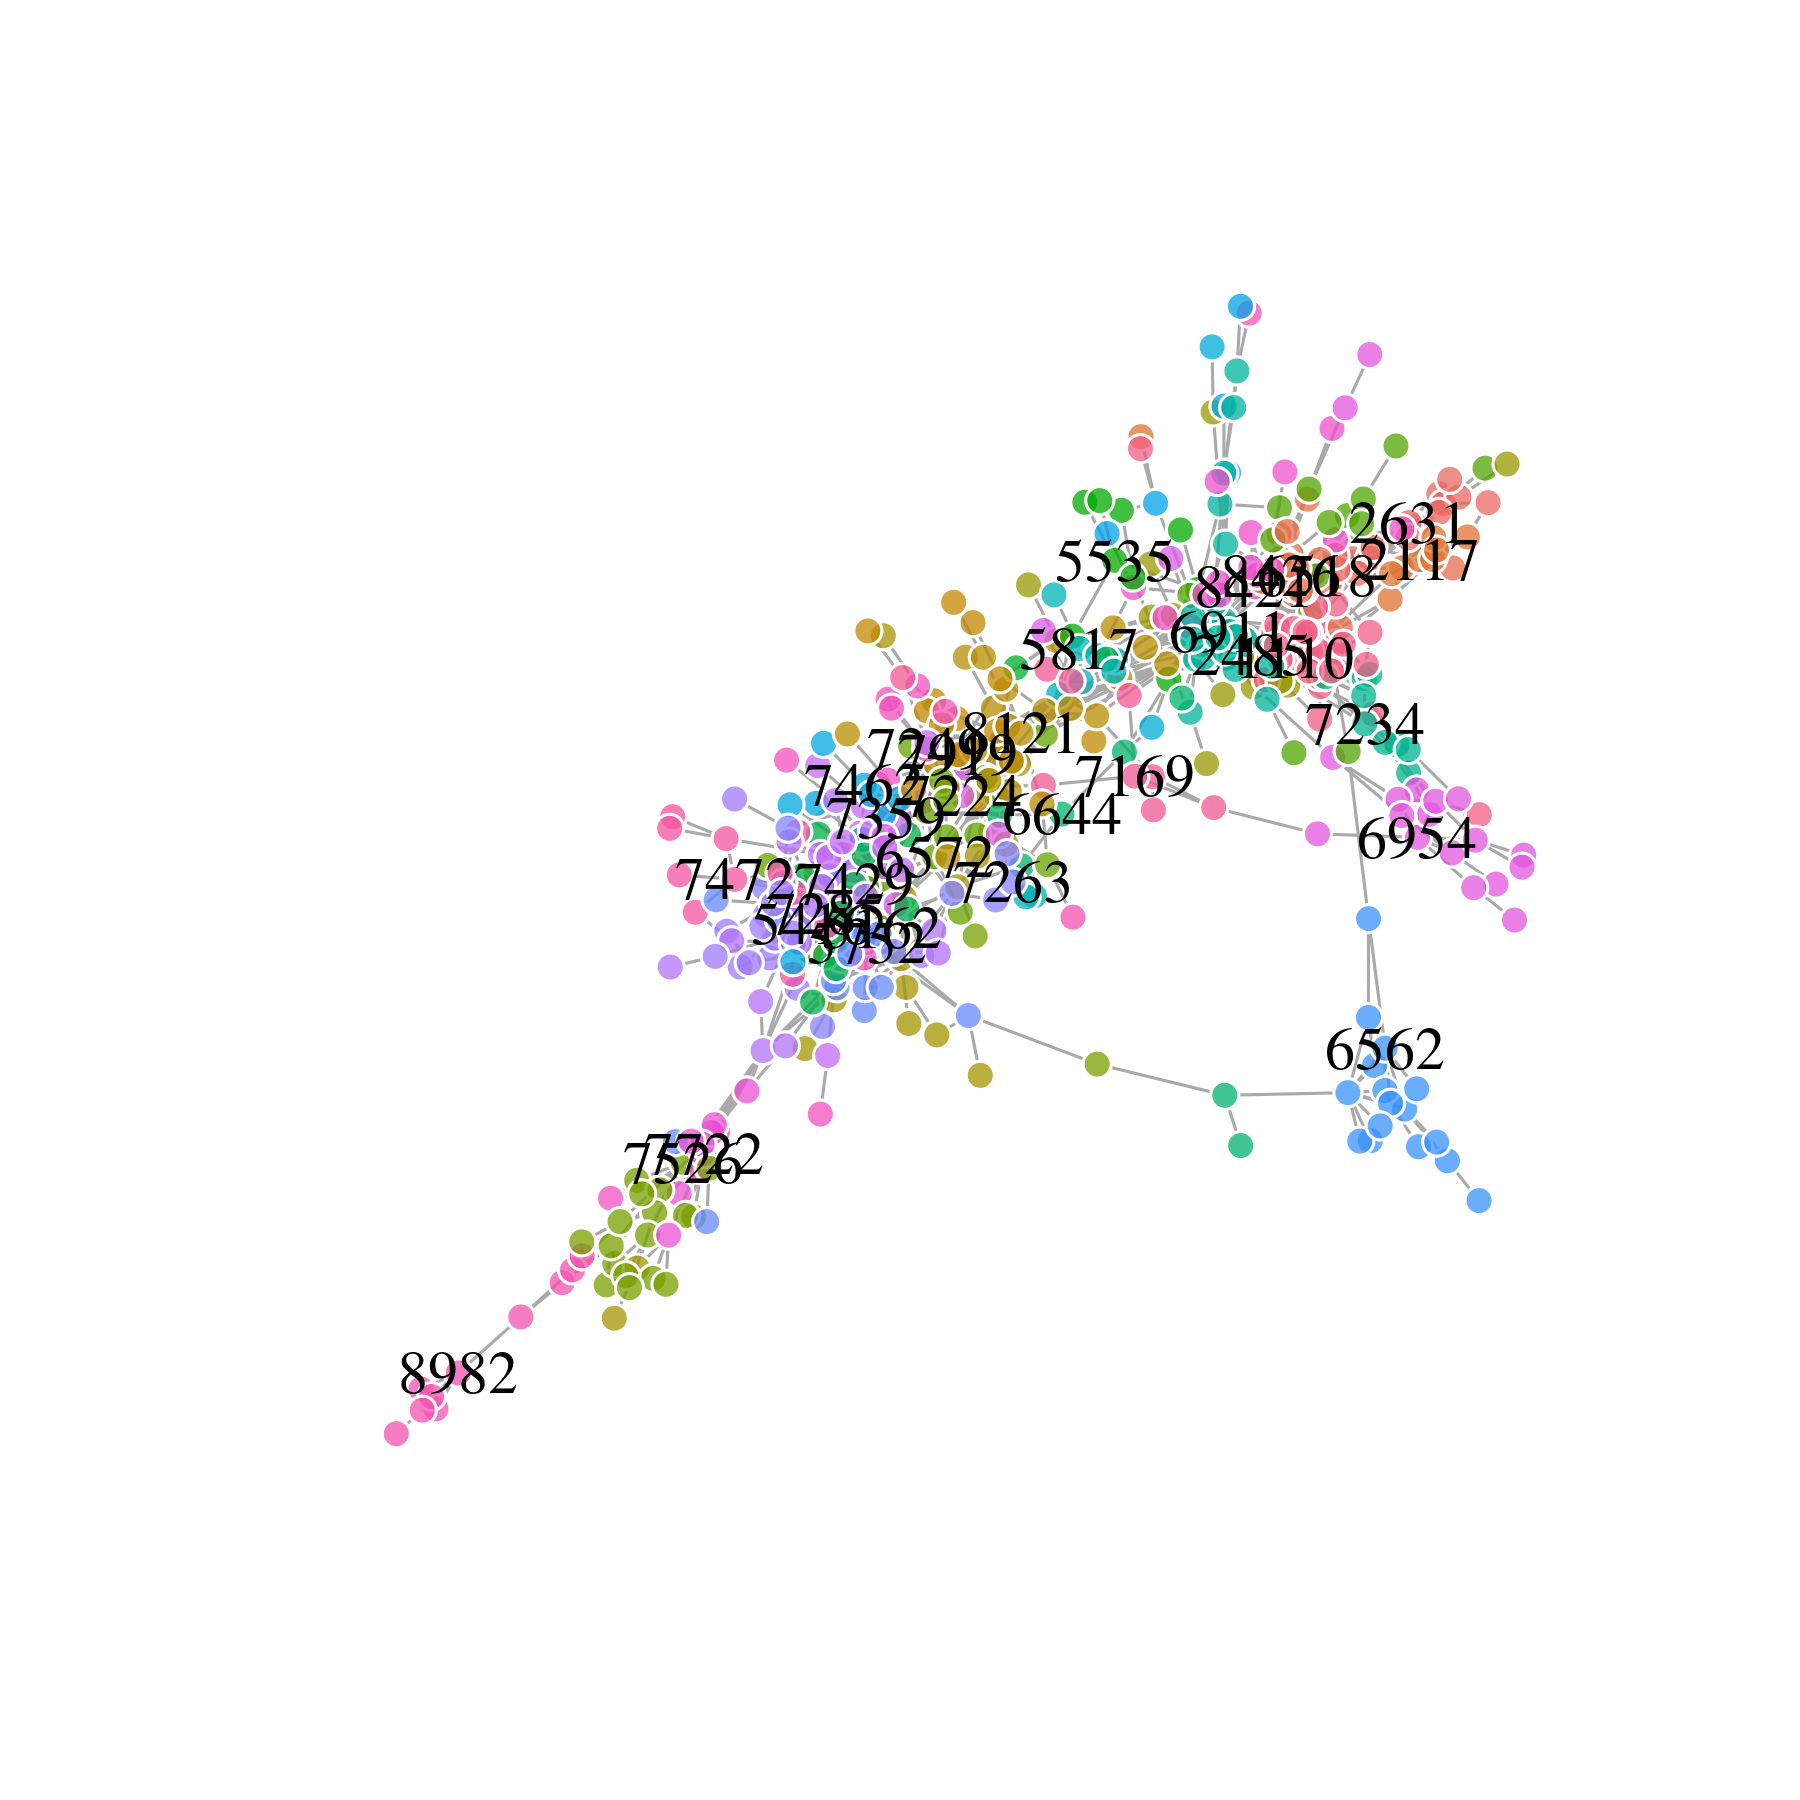
\includegraphics[width=\linewidth]{pam50_gigant}
	\caption{Componente gigante. Grafo de proximidad y clustering por K-medioides. Exportaciones. Promedio 1996-2017. 50 medioides}
	\label{fig:clustering50}
\end{figure}



\subsection{Conclusiones}





%\bibliographystyle{unsrt}
%\bibliography{bibliografia}
%
\end{document}

